% !BIB program = biber
% !TeX program = xelatex
\documentclass[12pt, a4paper, twoside, openany]{report}

% ── Encodage (XeLaTeX) ──────────────────────────────────────
\usepackage{fontspec}
\setmainfont{TeX Gyre Termes}
\setsansfont{TeX Gyre Termes}
\renewcommand{\familydefault}{\sfdefault}

% ── Mise en page (charte ENSA) ──────────────────────────────
\usepackage[a4paper,
            top=2.5cm, bottom=2.5cm,
            left=2.5cm, right=2.5cm]{geometry}
\usepackage{setspace}
\onehalfspacing
\setlength{\parskip}{6pt}
\setlength{\parindent}{0pt}

% ── Couleurs ────────────────────────────────────────────────
\usepackage[table]{xcolor}
\definecolor{titreBleu}{HTML}{1034A6}
\definecolor{headerBleu}{HTML}{D6E4F0}
\definecolor{rowGris}{HTML}{D0D0D0}
\definecolor{borderGris}{HTML}{BBBBBB}

% ── Figures et tableaux ─────────────────────────────────────
\usepackage{graphicx}
\usepackage{float}
\usepackage{booktabs}
\usepackage{multirow}
\usepackage{array}
\usepackage{longtable}
\usepackage{caption}
\usepackage{colortbl}

% ── Numérotation figures/tableaux/équations par chapitre ────
\usepackage{chngcntr}
\counterwithin{figure}{chapter}
\counterwithin{table}{chapter}
\counterwithin{equation}{chapter}

% ── Mathématiques ───────────────────────────────────────────
\usepackage{amsmath}
\usepackage{amssymb}

% ── Code source ─────────────────────────────────────────────
\usepackage{listings}
\lstset{
  basicstyle=\ttfamily\small,
  breaklines=true,
  frame=single,
  numbers=left,
  numberstyle=\tiny,
  keywordstyle=\color{blue},
  commentstyle=\color{gray},
  stringstyle=\color{red!70!black},
}

% ── Rotation de figures ─────────────────────────────────────
\usepackage{rotating}

% ── Diagrammes et planning ──────────────────────────────────
\usepackage{tikz}
\usetikzlibrary{arrows.meta, fit, positioning, shapes.geometric, shapes.multipart, calc}
\usepackage{pgfgantt}
\usepackage[edges]{forest}
\usepackage[most]{tcolorbox}

% ── En-têtes et pieds de page (charte) ──────────────────────
\usepackage{fancyhdr}
\pagestyle{fancy}
\fancyhf{}
\fancyhead[L]{%
  \begin{tikzpicture}[baseline=-0.5ex]
    \node[inner sep=0, opacity=0.5]
      {
\includegraphics[height=0.75cm]{logo-ensa.png}};
  \end{tikzpicture}%
}
\fancyhead[R]{\small\color{titreBleu}\itshape
  Framework ETL \`a Gateways de D\'ecision pour l'Import ERP Axelor}
\fancyfoot[L]{\small ENSA K\'enitra, Fili\`ere G\'enie Informatique}
\fancyfoot[R]{\small\thepage}
\renewcommand{\headrulewidth}{0.4pt}
\renewcommand{\footrulewidth}{0.4pt}
\setlength{\headheight}{28pt}
\addtolength{\topmargin}{-14pt}

% ── Titres de chapitres : package chargé ici, formats définis après bidi ──
\usepackage{titlesec}

\raggedbottom

% ── Liens internes ──────────────────────────────────────────
\usepackage[hidelinks]{hyperref}

% ── Bibliographie style IEEE ─────────────────────────────────
\usepackage[backend=biber, style=ieee, sorting=none, defernumbers=true]{biblatex}
\addbibresource{bibliographie.bib}

\graphicspath{{images/}}

% ── Polyglossia + arabe (charge bidi qui patche titlesec) ───
\usepackage{polyglossia}
\setmainlanguage{french}
\setotherlanguage[calendar=gregorian]{arabic}
\newfontfamily\arabicfont[Script=Arabic, Scale=1.2]{Amiri}
\newfontfamily\arabicfontsf[Script=Arabic, Scale=1.2]{Amiri}
\newfontfamily\arabicfonttt[Script=Arabic, Scale=1.2]{Amiri}

% ── Formats de titres définis APRÈS bidi pour qu'ils ne soient pas écrasés ──
\titleformat{\chapter}[block]
  {\normalfont\fontsize{16}{19}\bfseries\sffamily\color{titreBleu}}
  {Chapitre \thechapter}{1em}{}
\titleformat{name=\chapter,numberless}[block]
  {\normalfont\fontsize{16}{19}\bfseries\sffamily\color{titreBleu}}
  {}{0pt}{}
\titlespacing*{\chapter}{0pt}{0pt}{12pt}
\titleformat{\section}{\large\bfseries\sffamily\color{titreBleu}}{\thesection}{1em}{}
\titleformat{\subsection}{\normalsize\bfseries\sffamily\color{titreBleu}}{\thesubsection}{1em}{}
\titleformat{\subsubsection}{\normalsize\sffamily\color{titreBleu}}{\thesubsubsection}{1em}{}

\begin{document}

% ── Page de garde (sans numérotation) ───────────────────────
\pagestyle{empty}
\newgeometry{left=2.5cm, right=2.5cm, top=2cm, bottom=2cm}
\begin{titlepage}
\setlength{\parskip}{0pt}

\definecolor{bandeauBleu}{HTML}{1034A6}

% ── Logos ───────────────────────────────────────────────────
\begin{minipage}[t]{0.45\textwidth}
  \raggedright
  
\includegraphics[height=2cm]{logo-ensa.png}
\end{minipage}
\hfill
\begin{minipage}[t]{0.45\textwidth}
  \raggedleft
  \raisebox{0.4cm}{
\includegraphics[height=1.1cm]{logo_axelor.png}}
\end{minipage}

\vspace{0.6cm}

% ── En-tête institutionnel ───────────────────────────────────
\begin{center}
  Royaume du Maroc\\[0.15cm]
  \textbf{Université Ibn Tofaïl}\\[0.1cm]
  \textbf{École Nationale des Sciences Appliquées de Kénitra}\\[0.3cm]
  {\color{bandeauBleu}\textbf{Filière : Génie Informatique}}
\end{center}

\vspace{0.5cm}

% ── Type de mémoire ──────────────────────────────────────────
\begin{center}
  \textbf{Mémoire de Projet de Fin d'Études}\\[0.1cm]
  \textit{Pour l'obtention du diplôme d'Ingénieur d'État}
\end{center}

\vspace{0.5cm}

% ── Titre du projet ──────────────────────────────────────────
\begin{tikzpicture}
  \node[draw=bandeauBleu, line width=0.8pt,
        inner sep=16pt, text width=\dimexpr\textwidth-40pt\relax, align=center] {
    {\large \textbf{\color{bandeauBleu}Conception d'un Framework ETL Générique pour\\l'Import de Données Axelor, Assisté par Agents IA Génératifs}}
  };
\end{tikzpicture}

\vspace{0.6cm}

% ── Étudiant ─────────────────────────────────────────────────
\begin{center}
  \textbf{Réalisé par :}\\[0.2cm]
  Taha GHAILAN
\end{center}

\vspace{0.4cm}

% ── Encadrants ───────────────────────────────────────────────
\begin{center}
  \textbf{Encadré par :}\\[0.25cm]
  Pr. Younès EL BOUZEKRI EL IDRISSI, encadrant pédagogique, ENSA Kénitra\\[0.1cm]
  M. Abderrahim AABANE, encadrant professionnel, Axelor
\end{center}

\vspace{0.5cm}

% ── Jury ─────────────────────────────────────────────────────
\begin{center}
  \textbf{Soutenu le 07 juillet 2026 devant le jury composé de :}\\[0.4cm]
  \renewcommand{\arraystretch}{1.4}
  \begin{tabular}{|p{11cm}|p{4.8cm}|}
    \hline
    Pr. Younès EL BOUZEKRI EL IDRISSI, Professeur de\newline l'Enseignement Supérieur, ENSA Kénitra & \textbf{Encadrant} \\
    \hline
    Pr. Ayoub AIT LAHCEN, Professeur de l'Enseignement\newline Supérieur, ENSA Kénitra             & \textbf{Rapporteur} \\
    \hline
    Pr. Aniss MOUMEN, Professeur de l'Enseignement Supérieur, ENSA Kénitra                 & \textbf{Rapporteur} \\
    \hline
  \end{tabular}
\end{center}

\vfill

% ── Année universitaire ──────────────────────────────────────
\begin{center}
  {\color{bandeauBleu}\textbf{Année universitaire : 2025/2026}}
\end{center}

\end{titlepage}
\restoregeometry


% ── Pages préliminaires (numérotation romaine) ──────────────
\pagestyle{fancy}
\pagenumbering{roman}
\setcounter{page}{1}

\chapter*{Dédicaces}
\addcontentsline{toc}{chapter}{Dédicaces}
\markboth{Dédicaces}{Dédicaces}

\vspace{2cm}

\begin{center}

\textit{À mes chers parents,}\\[0.3cm]
Pour votre amour inconditionnel et vos sacrifices silencieux tout au long de mon parcours. Pour tous ces trajets que vous avez pris en charge en silence, pour que la route entre chez nous et l'université ne soit jamais un obstacle, pour le panier préparé avec soin chaque semaine pour que je ne manque jamais de rien. Vous avez porté tout ce que je n'ai jamais eu à porter, et c'est grâce à vous que j'ai pu me consacrer pleinement à mes études. Ce travail est le fruit de votre dévouement bien avant d'être le mien.\\[1cm]

\textit{À mes frères,}\\[0.3cm]
Pour votre présence réconfortante, votre soutien sincère et votre aide au quotidien. Vous avez été ma force dans les moments difficiles et ma joie dans les moments de réussite. Merci d'avoir toujours été là.\\[1cm]

\textit{À mes amis,}\\[0.3cm]
Pour votre bienveillance et les nouvelles perspectives que vous m'avez apportées, qui ont contribué à faire de moi la personne que je suis aujourd'hui. Merci pour les souvenirs inoubliables et les meilleurs moments que j'aurais pu vivre.\\[1cm]

\textit{À nos enseignants,}\\[0.3cm]
Pour le savoir transmis avec soin, votre patience et votre engagement sincère. Merci d'avoir cru en nous, même quand nous n'y croyions pas nous-mêmes.

\end{center}

\chapter*{Remerciements}
\addcontentsline{toc}{chapter}{Remerciements}
\markboth{Remerciements}{Remerciements}

À l'achèvement de ce projet de fin d'études, je rends grâce à Allah qui m'a donné la force, la volonté et la détermination d'accomplir ce travail.

Je remercie profondément mon tuteur de stage, \textbf{M.~Aabane Abderrahim}, pour ses conseils avisés, son encadrement suivi et son aide pendant toute cette période de vie professionnelle.

Je tiens également à remercier mon responsable hiérarchique, \textbf{M.~Couderc Pierre}, pour la confiance qu'il témoigne à mon égard et ses judicieux conseils.

Je remercie également mon tuteur pédagogique, \textbf{Pr.~El Bouzekri El Idrissi Younes}, pour son suivi de qualité, ses remarques constructives et son encadrement.

Je remercie également \textbf{Mme~Oumaira Ilhame} et \textbf{Mme~Ajanna Mehdia}, membres du jury, de l'honneur qu'elles me font d'accepter de juger ce travail.

Je remercie toute l'équipe \textbf{Axelor Maroc} pour son accueil agréable, sa disponibilité et ses remarques intéressantes qui ont permis ma montée en compétences.

Je remercie aussi tous les professeurs et le personnel administratif de l'École Nationale des Sciences Appliquées de Kénitra, pour la qualité de l'enseignement prodigué.

Pour finir, je remercie toute personne qui de près ou de loin a contribué à la réalisation de ce travail.

\chapter*{Résumé}
\addcontentsline{toc}{chapter}{Résumé}
\markboth{Résumé}{Résumé}

La migration de données constitue l'un des défis les plus critiques lors du déploiement d'un ERP. Dans le contexte d'Axelor Open Suite, ce processus repose actuellement sur des scripts Java développés spécifiquement pour chaque projet client — une approche coûteuse, non réutilisable et difficile à maintenir.

Ce mémoire présente la conception et le développement d'un framework ETL générique à gateways de décision, basé sur Apache Hop, destiné à standardiser et automatiser l'import de données vers Axelor. Le framework formalise les règles métier de l'ERP en transformations déclaratives et réutilisables, couvrant quatre domaines fonctionnels de complexité croissante : produits, partenaires, commandes et factures.

La solution intègre deux contributions complémentaires : (1) une architecture de pipeline à gateways avec résolution automatique des dépendances inter-entités, opérant en totale autonomie vis-à-vis de l'API Axelor ; (2) un pattern d'\textit{Agent-Assisted ETL} composé de 3 skills IA spécialisées et d'une application web (\textit{Axelor Mapper}) qui automatisent le cycle complet d'import — de l'analyse interactive du schéma source à la génération de pipelines conformes.

L'évaluation du framework sur quatre domaines fonctionnels démontre la capacité à importer des entités de complexité croissante, avec un gain de productivité significatif sur les phases de configuration grâce à l'assistance IA.

\textbf{Mots clés :} ETL, Apache Hop, ERP, Axelor, Pipeline à Gateways, Migration de Données, LLM, Agent IA, Génération de Code.

\chapter*{Abstract}
\addcontentsline{toc}{chapter}{Abstract}
\markboth{Abstract}{Abstract}

Data migration is one of the most critical challenges when deploying an ERP system. In the context of Axelor Open Suite, this process currently relies on Java scripts developed specifically for each client project — a costly, non-reusable approach that is difficult to maintain.

This report presents the design and development of a generic decision-gateway ETL framework, built on Apache Hop, aimed at standardising and automating data import into Axelor. The framework formalises the ERP's business rules as declarative, reusable transformations, covering four functional domains of increasing complexity: products, partners, orders, and invoices.

The solution delivers two complementary contributions: (1) a gateway-based pipeline architecture with automatic inter-entity dependency resolution, operating fully independently from the Axelor API; (2) an \textit{Agent-Assisted ETL} pattern comprising 3 specialised AI skills and a web application (\textit{Axelor Import Studio}) that automate the full import cycle — from interactive source schema analysis to compliant pipeline generation.

Evaluation of the framework across four functional domains demonstrates the ability to import entities of increasing complexity, with significant productivity gains on configuration phases through AI assistance.

\textbf{Keywords:} ETL, Apache Hop, ERP, Axelor, Gateway Pipeline, Data Migration, LLM, AI Agent, Code Generation.

\begin{Arabic}
\chapter*{ملخص}
\addcontentsline{toc}{chapter}{{\arabicfont ملخص}}

\vspace{0.5cm}

تُعدّ عملية ترحيل البيانات من أبرز التحديات التقنية عند نشر نظام تخطيط موارد المؤسسات. في سياق منصة Axelor Open Suite، تعتمد هذه العملية حالياً على برامج Java مخصصة لكل مشروع عميل — وهو نهج مكلف وغير قابل لإعادة الاستخدام وصعب الصيانة.

يقدّم هذا التقرير تصميم وتطوير إطار عمل ETL عام قائم على بوابات القرار، مبني على Apache Hop، يهدف إلى توحيد وأتمتة استيراد البيانات نحو Axelor. يُشكّل هذا الإطار قواعد العمل الخاصة بنظام ERP في تحويلات تصريحية قابلة لإعادة الاستخدام، تغطي أربعة مجالات وظيفية متزايدة التعقيد: المنتجات، الشركاء، أوامر البيع والفواتير.

يقدّم الحل مساهمتين متكاملتين: (1) بنية أنابيب قائمة على بوابات القرار مع حل تلقائي للتبعيات بين الكيانات، تعمل باستقلالية تامة عن واجهة برمجة تطبيقات Axelor؛ (2) نمط ETL بمساعدة الذكاء الاصطناعي يتألف من 3 مهارات ذكاء اصطناعي متخصصة وتطبيق ويب (Axelor Mapper) يؤتمت دورة الاستيراد الكاملة — من التحليل التفاعلي لمخطط المصدر إلى توليد الأنابيب المتوافقة.

\textbf{الكلمات المفتاحية:} ETL، Apache Hop، ERP، Axelor، أنابيب بوابات القرار، ترحيل البيانات، نموذج لغوي كبير، وكيل ذكاء اصطناعي، توليد الشيفرة.

\end{Arabic}

\chapter*{Liste des abréviations}
\addcontentsline{toc}{chapter}{Liste des abréviations}
\markboth{Liste des abréviations}{Liste des abréviations}

\begin{table}[H]
  \centering
  \renewcommand{\arraystretch}{1.4}
  \begin{tabular}{p{3cm} p{10cm}}
    \toprule
    \rowcolor{gray!20}
    \textbf{Abréviation} & \textbf{Signification} \\
    \midrule
    \rowcolor{gray!5}
    AOP     & Axelor Open Platform \\
    AOS     & Axelor Open Suite \\
    \rowcolor{gray!5}
    API     & Application Programming Interface \\
    BPM     & Business Process Management \\
    \rowcolor{gray!5}
    CLI     & Command Line Interface \\
    CRM     & Customer Relationship Management \\
    \rowcolor{gray!5}
    CSV     & Comma-Separated Values \\
    ERP     & Enterprise Resource Planning \\
    \rowcolor{gray!5}
    ETL     & Extract, Transform, Load \\
    FK      & Foreign Key (clé étrangère) \\
    \rowcolor{gray!5}
    HOP     & Hop Orchestration Platform (Apache Hop) \\
    IA      & Intelligence Artificielle \\
    \rowcolor{gray!5}
    JSON    & JavaScript Object Notation \\
    LLM     & Large Language Model \\
    \rowcolor{gray!5}
    PTY     & Pseudo-Terminal \\
    REST    & Representational State Transfer \\
    \rowcolor{gray!5}
    SQL     & Structured Query Language \\
    SSE     & Server-Sent Events \\
    \rowcolor{gray!5}
    UML     & Unified Modeling Language \\
    XML     & Extensible Markup Language \\
    \rowcolor{gray!5}
    WS      & WebSocket \\
    \bottomrule
  \end{tabular}
\end{table}


\listoffigures
\clearpage

\listoftables
\clearpage

\tableofcontents
\clearpage

% ── Corps du rapport (numérotation arabe) ───────────────────
\pagenumbering{arabic}
\setcounter{page}{1}

\chapter*{Introduction Générale}
\addcontentsline{toc}{chapter}{Introduction Générale}
\markboth{Introduction Générale}{Introduction Générale}

\vspace{0.5cm}

Dans un contexte économique en perpétuelle évolution, les entreprises sont confrontées à une pression croissante liée à la digitalisation de leurs processus. Les systèmes ERP (Enterprise Resource Planning) occupent une place centrale dans cette transformation, en centralisant l'ensemble des processus métier au sein d'un système unique et cohérent. Cependant, le déploiement d'un ERP soulève invariablement une problématique critique : la migration des données historiques depuis les systèmes legacy du client.

C'est dans ce contexte que s'inscrit ce projet de fin d'études, réalisé au sein d'\textit{Axelor}, éditeur français d'une plateforme ERP-CRM-BPM open source. Face à la multiplication des projets clients et à la complexité croissante des données à migrer, Axelor fait face à une limitation structurelle : chaque déploiement nécessite le développement de scripts Java sur mesure, non réutilisables et difficiles à maintenir.

L'objectif principal de ce stage est de concevoir et développer un \textbf{framework ETL générique à gateways de décision}, basé sur Apache Hop, capable de formaliser les règles métier d'Axelor en transformations déclaratives et réutilisables. Plus précisément, le projet vise à :

\begin{itemize}
  \item \textbf{Standardiser} le processus d'import de données en remplaçant les scripts Java ad hoc par des pipelines ETL paramétrables et versionnables ;
  \item \textbf{Couvrir} quatre domaines fonctionnels de complexité croissante : produits, partenaires, commandes de vente et factures ;
  \item \textbf{Automatiser} les phases de configuration et de génération de pipelines via des skills IA spécialisées (agents génératifs) ;
  \item \textbf{Développer} une application web (\textit{Axelor Mapper}) offrant une interface conversationnelle entre le consultant et l'agent IA pour le mapping des données.
\end{itemize}

Ce mémoire est structuré en sept chapitres :

\begin{itemize}
  \item \textbf{Chapitre 1} présente l'organisme d'accueil Axelor et le déroulement du stage.
  \item \textbf{Chapitre 2} expose le contexte du projet, la problématique et l'organisation du travail.
  \item \textbf{Chapitre 3} formalise le cadrage du besoin, les exigences fonctionnelles et non fonctionnelles, la méthodologie adoptée et le planning de réalisation.
  \item \textbf{Chapitre 4} présente la conception fonctionnelle à travers les diagrammes UML.
  \item \textbf{Chapitre 5} détaille l'architecture technique, le benchmark des technologies et les choix retenus.
  \item \textbf{Chapitre 6} décrit l'implémentation des pipelines ETL, des skills IA et de l'application Axelor Mapper.
  \item \textbf{Chapitre 7} présente les résultats obtenus, les tests de validation et le bilan du projet.
\end{itemize}

\chapter{Contexte général du projet}
\label{chap:contexte}

Ce premier chapitre a pour objectif de situer le cadre général dans lequel s'inscrit notre projet de fin d'études. Nous commençons par présenter l'organisme d'accueil, puis nous exposons le contexte et la problématique qui ont motivé ce travail, avant de détailler l'organisation adoptée pour sa réalisation.

%% ─────────────────────────────────────────────
\section{Présentation de l'organisme d'accueil}
\label{sec:organisme}
%% ─────────────────────────────────────────────

\subsection{Fiche technique}

\begin{table}[H]
  \centering
  \renewcommand{\arraystretch}{1.5}
  \begin{tabular}{p{4.5cm} p{9.5cm}}
    \toprule
    \rowcolor{gray!20}
    \textbf{Champ} & \textbf{Information} \\
    \midrule
    \rowcolor{gray!5}
    \textbf{Raison sociale}     & Axelor SAS \\
    \textbf{Date de création}   & 2005 \\
    \rowcolor{gray!5}
    \textbf{PDG}                & Laith Jubair \\
    \textbf{Siège social}       & Marne-la-Vallée, France \\
    \rowcolor{gray!5}
    \textbf{Secteur d'activité} & Édition de logiciels ERP/CRM/BPM \\
    \textbf{Filiales}           & Inde, Maroc, Canada \\
    \rowcolor{gray!5}
    \textbf{Produits phares}    & Axelor Open Platform (AOP), Axelor Open Suite (AOS) \\
    \textbf{Licence}            & Open Source (AGPLv3) \\
    \rowcolor{gray!5}
    \textbf{Site web}           & \url{https://www.axelor.com/} \\
    \bottomrule
  \end{tabular}
  \caption{Fiche technique d'Axelor}
  \label{tab:fiche-technique}
\end{table}

\subsection{Présentation générale}

Axelor est un éditeur français de logiciels open source spécialisé dans les solutions ERP, CRM et BPM. Fondée en 2005 et dirigée par Laith Jubair (PDG), l'entreprise propose une plateforme complète permettant aux organisations de digitaliser et d'optimiser l'ensemble de leurs processus métier. Axelor se distingue par son approche open source et sa philosophie low-code, rendant ses solutions accessibles à un large éventail d'entreprises~\cite{axelor_erp}.

Implantée dans quatre pays, Axelor dispose de 7 sites en France (siège social), au Maroc, au Canada et en Inde.

\begin{figure}[H]
  \centering
  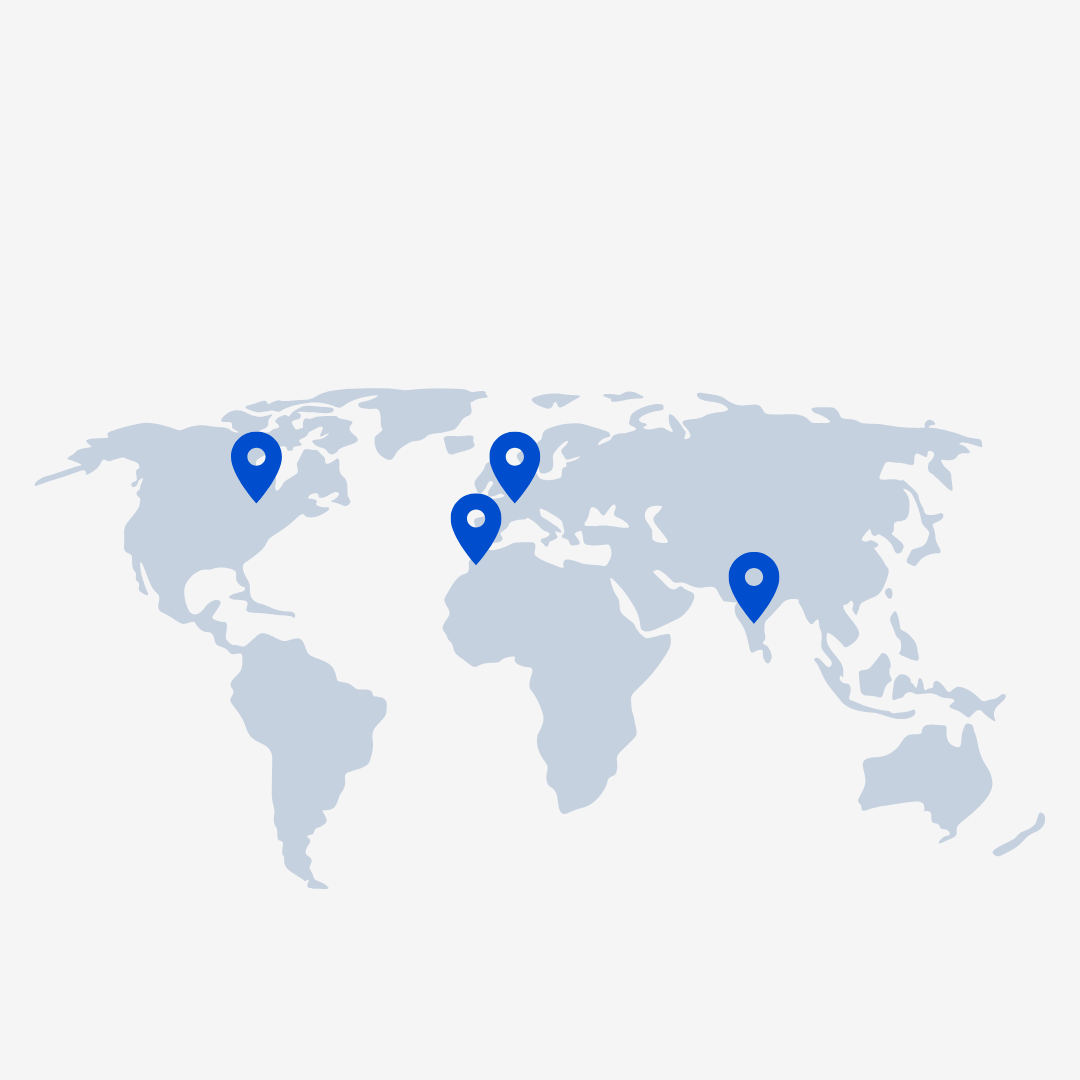
\includegraphics[width=0.85\textwidth]{Siege-Axelor.png}
  \caption{Implantations géographiques d'Axelor dans le monde}
  \label{fig:siege-axelor}
\end{figure}

\subsection{Secteur d'activité}

Axelor évolue dans le secteur de l'édition de logiciels de gestion d'entreprise. Son cœur de métier couvre trois domaines complémentaires :
\begin{itemize}
    \item \textbf{ERP} — Progiciel de Gestion Intégré couvrant la comptabilité, les achats, les ventes, la production et les stocks ;
    \item \textbf{CRM} — Gestion de la Relation Client pour le suivi commercial et marketing ;
    \item \textbf{BPM} — Gestion des Processus Métier pour la modélisation et l'automatisation des workflows.
\end{itemize}

\subsection{Structure et organisation}

L'organigramme de la filiale Axelor Maroc illustre une structure hiérarchique claire. Sous la direction générale, l'organisation s'articule autour d'un directeur de projet supervisant les chefs de projet, lesquels encadrent les consultants fonctionnels et les ingénieurs R\&D. Une responsable des ressources humaines complète cette structure. Cette organisation permet une coordination efficace entre les équipes techniques et fonctionnelles pour la livraison des projets d'intégration ERP.

\begin{figure}[H]
  \centering
  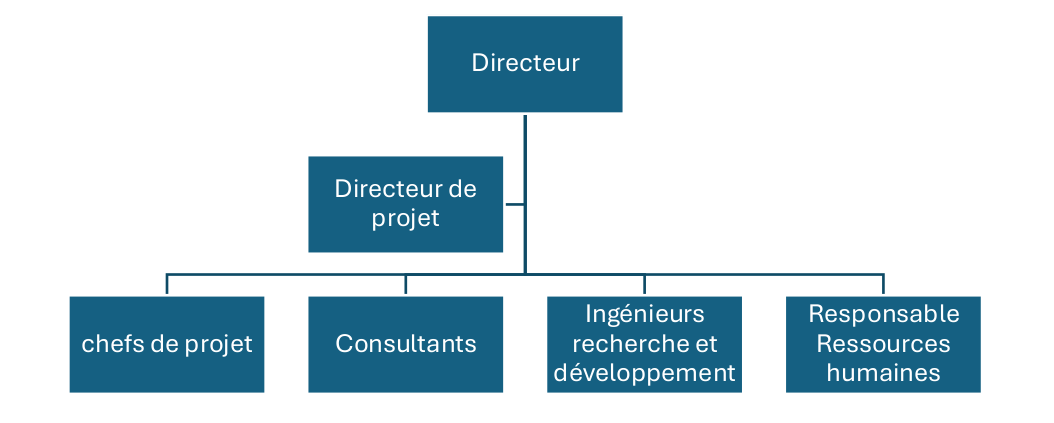
\includegraphics[width=0.85\textwidth]{organigramme-axelor-maroc.png}
  \caption{Organigramme d'Axelor Maroc}
  \label{fig:organigramme-axelor}
\end{figure}

\subsection{Stack technique}

La plateforme Axelor repose sur une architecture multi-couches s'appuyant sur des technologies éprouvées :

\begin{itemize}
    \item \textbf{Interface utilisateur} — React pour le frontend web moderne et réactif ;
    \item \textbf{Web Services} — RESTEasy pour l'exposition d'API RESTful ;
    \item \textbf{Sécurité} — Apache Shiro pour l'authentification et le contrôle d'accès ;
    \item \textbf{Reporting / BI} — BIRT pour la génération de rapports et tableaux de bord ;
    \item \textbf{Processus} — Camunda pour la modélisation et l'exécution des workflows BPM ;
    \item \textbf{Modules métier} — Java pour la logique applicative ;
    \item \textbf{ORM} — Hibernate pour la persistance objet-relationnelle~\cite{hibernate2024} ;
    \item \textbf{Base de données} — PostgreSQL comme SGBD relationnel~\cite{postgresql_doc}.
\end{itemize}

\begin{figure}[H]
  \centering
  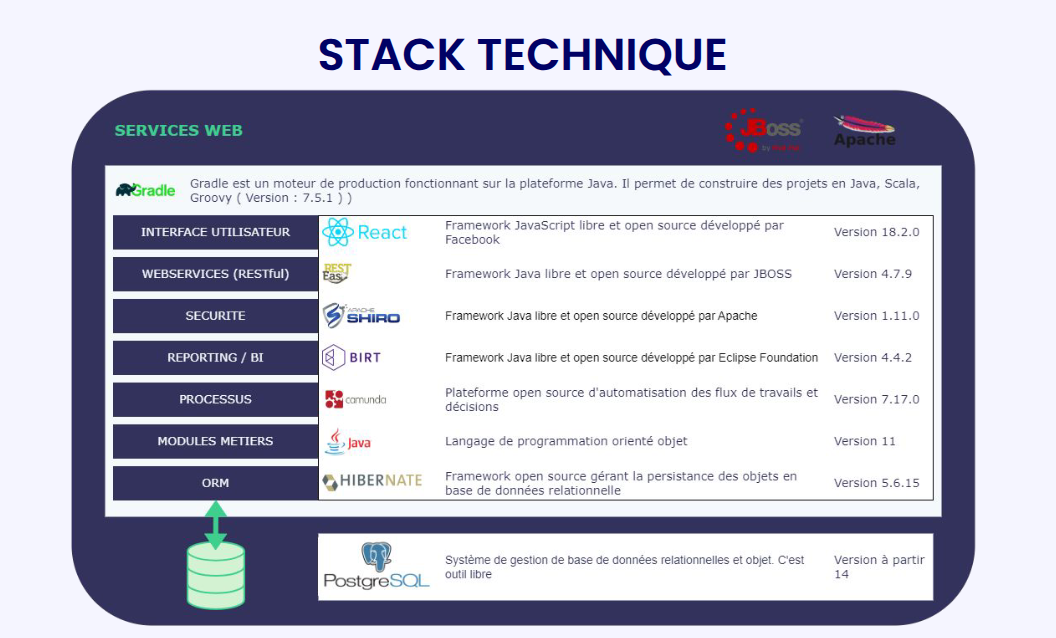
\includegraphics[width=\textwidth]{stack-technique.png}
  \caption{Stack technique de la plateforme Axelor}
  \label{fig:stack-technique}
\end{figure}

\subsection{Produits}

L'offre d'Axelor s'articule autour de deux composantes principales :

\begin{itemize}
    \item \textbf{Axelor Open Platform (AOP)} — Une plateforme low-code permettant de développer rapidement des applications métier grâce à un système de description déclarative (XML) et à un moteur de vues dynamiques ;
    \item \textbf{Axelor Open Suite (AOS)} — Un ensemble de plus de 30 applications métier intégrées construites sur AOP, couvrant la comptabilité, la gestion commerciale, les ressources humaines, la production, la supply chain, et bien d'autres domaines.
\end{itemize}

\subsection{Clients}

Axelor accompagne une clientèle diversifiée, allant des PME aux grands groupes internationaux, dans des secteurs tels que l'industrie, l'énergie, le e-commerce et le secteur public. Parmi les références notables figurent \textbf{Thyssenkrupp}, \textbf{Stellantis}, \textbf{Cdiscount}, \textbf{Trenitalia}, \textbf{Enercoop}, \textbf{Carbone~4}, ainsi que des institutions publiques comme le \textbf{Ministère de la Justice} et le \textbf{Conseil départemental des Hauts-de-Seine}. L'écosystème Axelor compte aujourd'hui plus d'un million d'utilisateurs à travers le monde.

\begin{figure}[H]
  \centering
  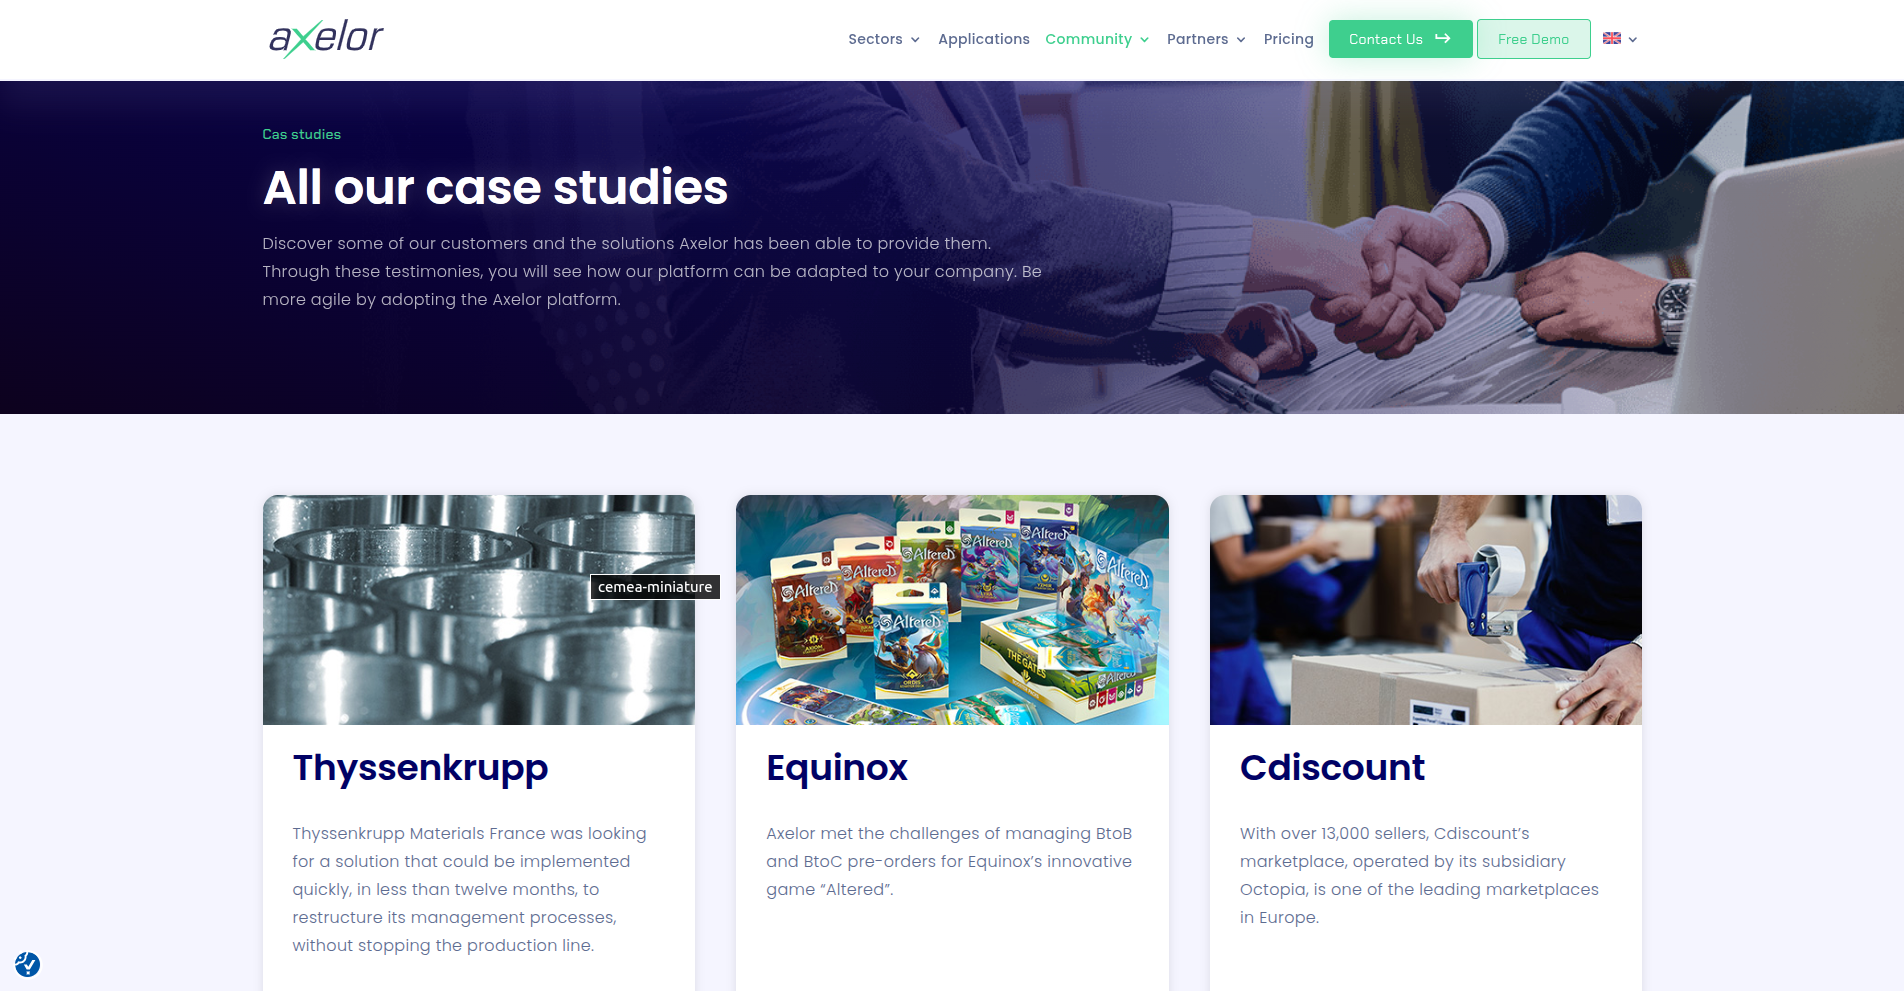
\includegraphics[width=0.9\textwidth]{axelor-clients1.png}\\[0.3cm]
  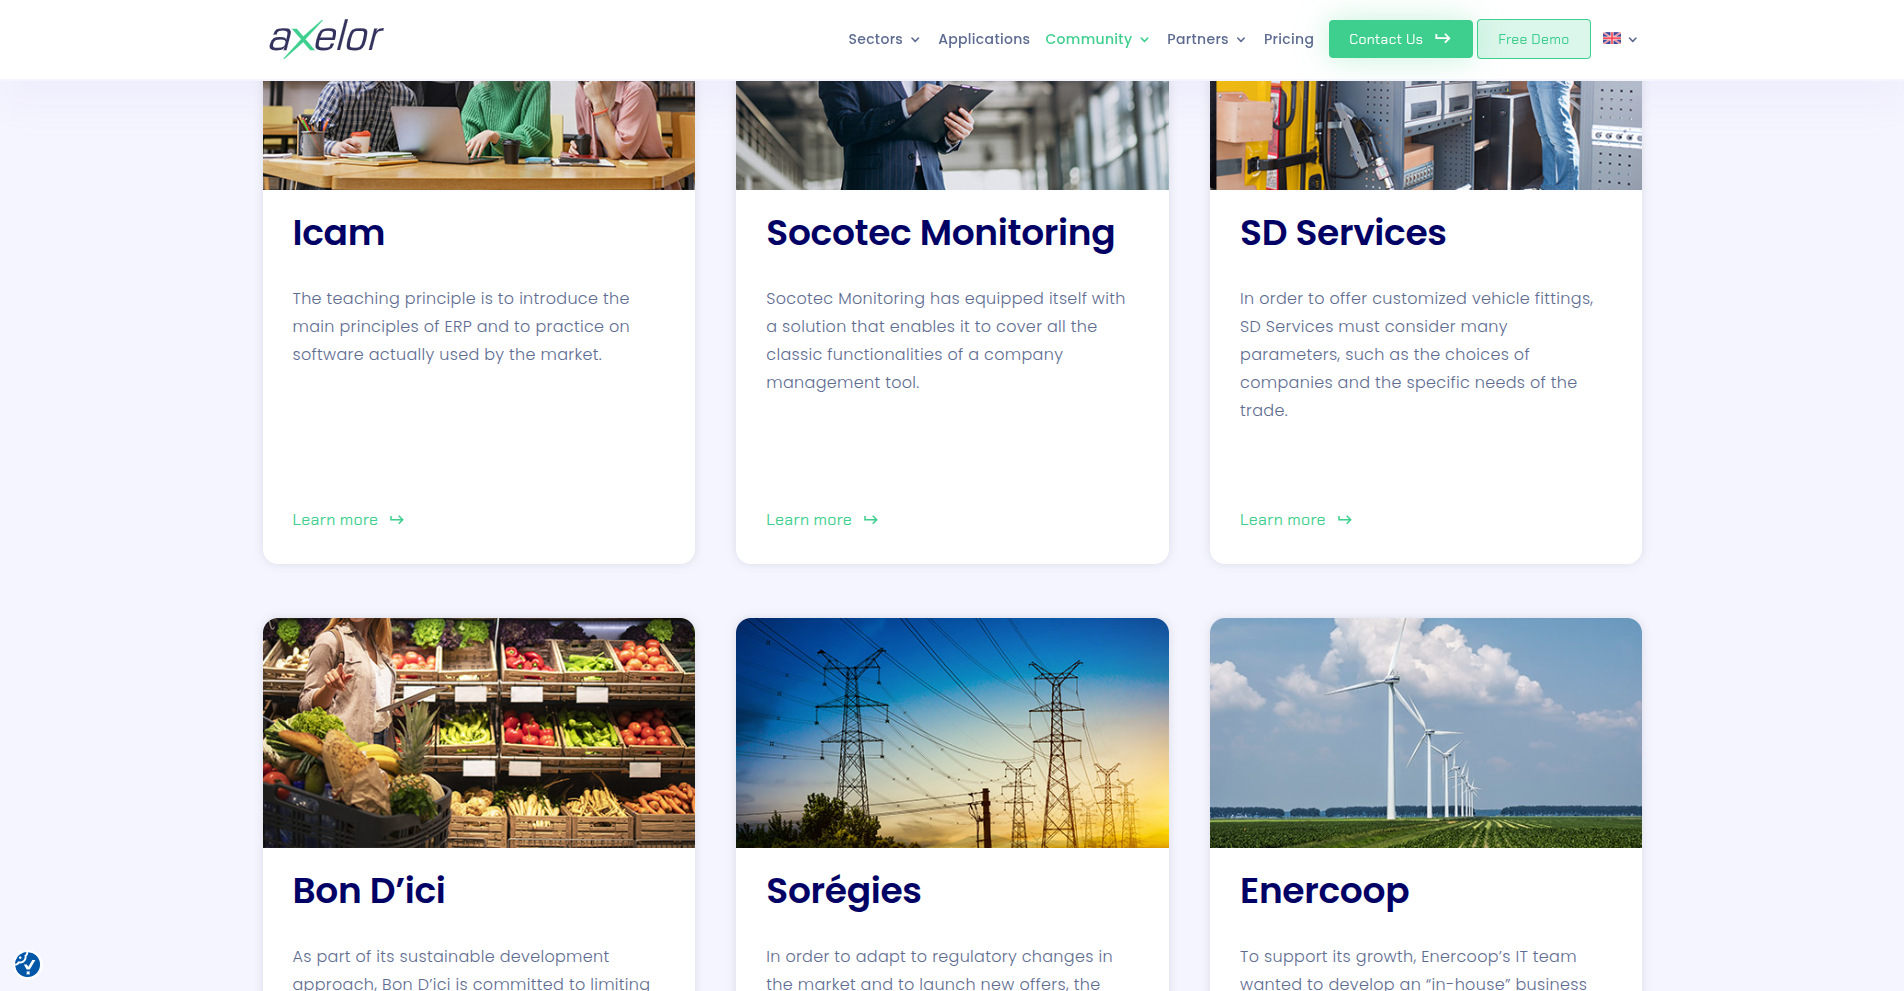
\includegraphics[width=0.9\textwidth]{axelor-clients2.png}
  \caption{Principaux clients d'Axelor}
  \label{fig:clients-axelor}
\end{figure}

%% ─────────────────────────────────────────────
\section{Contexte et enjeux du projet}
\label{sec:contexte-enjeux}
%% ─────────────────────────────────────────────

Axelor accompagne ses clients — PME, ETI et grands groupes — dans la mise en place de son ERP open source. Ces clients évoluent dans des secteurs variés (industrie, services, énergie, e-commerce) et disposent chacun de données historiques issues de systèmes d'information hétérogènes : anciens ERP, fichiers Excel, bases de données propriétaires ou exports CSV manuels.

Lors de chaque nouveau déploiement, la phase de \textbf{migration de données} constitue une étape incontournable et critique. Elle conditionne la mise en production de l'ERP car le client ne peut basculer vers Axelor qu'une fois l'intégralité de ses données de référence (produits, clients, fournisseurs, historiques de commandes et de factures) importée et vérifiée dans le nouveau système.

Aujourd'hui, cette migration repose sur le développement de \textbf{scripts Java spécifiques} pour chaque projet. L'équipe d'intégration développe en moyenne plus de 20 scripts par client, chacun dédié à l'import d'une entité métier donnée. Ces scripts interagissent avec l'API REST d'Axelor ou écrivent directement en base.

Cette approche pose plusieurs \textbf{enjeux stratégiques} pour Axelor :
\begin{itemize}
    \item \textbf{Coût élevé par projet} — le développement de scripts sur mesure mobilise des ressources d'ingénierie significatives, allongeant le délai de mise en production ;
    \item \textbf{Absence de capitalisation} — les scripts d'un projet ne sont pas réutilisables sur le suivant, même lorsque les structures de données sont similaires ;
    \item \textbf{Dépendance à un profil technique} — seuls les développeurs Java maîtrisant le modèle de données AOS peuvent réaliser ces imports, créant un goulot d'étranglement ;
    \item \textbf{Frein à la scalabilité} — avec la croissance du nombre de clients, cette approche artisanale ne passe pas à l'échelle.
\end{itemize}

%% ─────────────────────────────────────────────
\section{Présentation du projet}
\label{sec:presentation-projet}
%% ─────────────────────────────────────────────

Ce projet de fin d'études vise à concevoir et développer un framework ETL générique, assisté par intelligence artificielle, pour automatiser l'import de données vers Axelor Open Suite. Le framework couvre quatre domaines fonctionnels de complexité croissante (produits, partenaires, commandes de vente, factures) et intègre une application web permettant aux consultants de configurer les imports sans compétence Java.

Le stagiaire est intégré dans l'équipe R\&D d'Axelor Maroc en tant qu'ingénieur R\&D, sous l'encadrement technique quotidien de M.~Abderrahim Aabane et la supervision projet de M.~Pierre Couderc. Il est responsable de l'intégralité du cycle de développement : conception, implémentation, tests et validation du framework.

%% ─────────────────────────────────────────────
\section{Déroulement du stage}
\label{sec:deroulement}
%% ─────────────────────────────────────────────

Le stage s'est déroulé du \textbf{16 février 2026} au \textbf{31 juillet 2026} au sein de l'équipe R\&D d'\textit{Axelor Maroc}.
Le tableau~\ref{tab:deroulement} présente les principales phases du stage dans l'ordre chronologique.

\begin{table}[H]
  \centering
  \renewcommand{\arraystretch}{1.5}
  \begin{tabular}{p{3.5cm} p{3.5cm} p{7cm}}
    \toprule
    \rowcolor{gray!20}
    \textbf{Période} & \textbf{Phase} & \textbf{Activités principales} \\
    \midrule
    \rowcolor{gray!5}
    Semaines 1--6    & Formation technique   & Formation sur le framework AOP (Axelor Open Platform), architecture modulaire, mécanismes d'import \\
    \midrule
    \multicolumn{3}{l}{\textit{À partir de la semaine 7, répartition 50\% PFE / 50\% projets clients Axelor}} \\
    \midrule
    \rowcolor{gray!5}
    Semaines 7--10   & Pipelines ETL         & Conception et création des pipelines Apache Hop pour les 4 entités principales \\
    Semaines 11--14  & Application Mapper    & Développement de l'application Axelor Mapper (backend + frontend + agent IA) \\
    \rowcolor{gray!5}
    Semaines 15--18  & Skills IA             & Développement des skills Claude (analyse, mapping, génération de pipelines) \\
    Semaines 19--20  & Tests \& validation   & Tests end-to-end, validation sur un golden dataset \\
    \bottomrule
  \end{tabular}
  \caption{Déroulement chronologique du stage}
  \label{tab:deroulement}
\end{table}

\textit{Note :} À partir de la semaine 7, le travail sur le projet PFE s'est effectué en parallèle d'une activité d'intégration sur des projets clients Axelor (50\% du temps sur chaque volet).

%% ─────────────────────────────────────────────
\section*{Conclusion}
%% ─────────────────────────────────────────────

Ce chapitre a présenté l'organisme d'accueil Axelor, son secteur d'activité et son organisation, avant d'exposer le contexte et les enjeux de la migration de données ERP. Nous avons ensuite introduit le projet et ses objectifs, ainsi que le déroulement du stage. Le chapitre suivant formule la problématique de manière détaillée et présente la solution proposée.

\chapter{Problématique}
\label{chap:problematique}

Ce chapitre analyse le système existant et ses limites, formule la problématique centrale du projet et présente la solution proposée.

%% ============================================================
\section{Critique de l'existant}
\label{sec:critique-existant}
%% ============================================================

Lors du déploiement d'Axelor Open Suite (AOS) chez un nouveau client, l'une des étapes les plus critiques est l'import des données depuis le système d'information existant. Les clients disposent de données historiques issues d'ERP hétérogènes, de fichiers CSV exportés manuellement, ou de bases de données propriétaires. Ces données ne sont souvent pas conformes au modèle de données d'AOS : formats de dates différents, clés étrangères manquantes, devises ou unités non référencées, adresses dans des formats libres, etc. La mise en conformité et l'injection de ces données dans la base Axelor représente un défi technique récurrent pour chaque projet d'intégration.

Lors de chaque déploiement, l'équipe d'intégration doit développer plus de 20 scripts Java spécifiques pour assurer l'import des données. Le tableau~\ref{tab:projets-scripts} illustre la réalité de quelques projets récents :

\begin{table}[H]
    \centering
    \renewcommand{\arraystretch}{1.3}
    \begin{tabular}{p{3cm} p{4.5cm} p{5cm}}
        \toprule
        \rowcolor{gray!20}
        \textbf{Projet} & \textbf{Scripts} & \textbf{Secteur} \\
        \midrule
        \rowcolor{gray!5}
        bolt-app & 23 scripts Java & Manufacturing \\
        neodyme  & 20 scripts Java & Services \\
        \rowcolor{gray!5}
        xelians  & 3 configs XML + scripts Python & Gestion documentaire \\
        \bottomrule
    \end{tabular}
    \caption{Volume de scripts d'import par projet client}
    \label{tab:projets-scripts}
\end{table}

Ces scripts sont écrits sur mesure pour chaque client et ne sont pas réutilisables d'un projet à l'autre.

Il est important de noter qu'Axelor dispose d'un mécanisme natif d'import de données, basé sur des fichiers de binding XML associés à des fichiers CSV. Ce système permet de définir des correspondances entre colonnes CSV et champs du modèle, de résoudre les relations (Many-to-One, Many-to-Many) via des critères de recherche, et d'exécuter des traitements Java personnalisés lors de l'import. Cependant, ce mécanisme passe par l'ensemble de la couche applicative d'Axelor (validations métier, listeners, calculs dérivés), ce qui engendre un \textbf{temps d'exécution significatif} lors de l'import de volumes importants. En contournant ce framework applicatif et en insérant directement dans PostgreSQL, notre solution élimine cette surcharge et réduit considérablement les temps d'import — tout en respectant l'intégrité du schéma de données.

L'approche actuelle présente plusieurs limites significatives :
\begin{itemize}
    \item \textbf{Coût élevé} — Le développement de scripts sur mesure mobilise des ressources de développement importantes pour chaque projet ;
    \item \textbf{Non-réutilisabilité} — Les scripts sont spécifiques à chaque client et ne capitalisent pas sur les projets précédents ;
    \item \textbf{Dépendance à un développeur Java} — Chaque projet d'intégration nécessite l'intervention d'un développeur Java qualifié ;
    \item \textbf{Performance limitée} — Le passage par la couche applicative Axelor (binding XML + traitements Java) ralentit significativement les imports à grande volumétrie.
\end{itemize}

%% ============================================================
\section{Motivation et problématique}
\label{sec:motivation}
%% ============================================================

\subsection{Motivation}

Plusieurs facteurs convergent pour rendre ce projet pertinent aujourd'hui :

\begin{itemize}
    \item \textbf{Maturité des outils ETL open source} — Apache Hop, issu du projet Kettle/Pentaho, offre désormais une plateforme stable avec plus de 400 transformations natives, un format XML versionnable et une exécution en ligne de commande compatible avec les pipelines CI/CD modernes.
    \item \textbf{Émergence des LLMs capables de générer du code} — Les modèles de langage de dernière génération (Claude, GPT-4) démontrent une capacité à produire du code structuré (XML, JSON) à partir d'instructions en langage naturel, ouvrant la voie à l'automatisation de tâches de configuration jusqu'ici manuelles.
    \item \textbf{Besoin de scalabilité chez Axelor} — Avec la croissance du nombre de projets clients, l'approche artisanale actuelle ne passe plus à l'échelle. Axelor a besoin d'un outil qui capitalise sur les projets passés et réduit le temps d'intégration par client.
\end{itemize}

\subsection{Formulation de la problématique}

La problématique centrale de notre projet se formule ainsi :

\begin{quote}
\textit{Comment concevoir un framework ETL générique qui formalise les règles métier de l'ERP sous forme de transformations déclaratives et accélère la configuration grâce à des agents d'intelligence artificielle ?}
\end{quote}

\subsection{Objectifs}

Pour répondre à cette problématique, nous avons défini les objectifs suivants :

\begin{enumerate}
    \item \textbf{Standardiser le processus d'import} — Remplacer les scripts Java ad hoc par des pipelines ETL déclaratifs, paramétrables et versionnables. Chaque pipeline doit implémenter un pattern d'upsert (insert ou update selon l'existence de l'enregistrement) garantissant l'idempotence des imports.

    \item \textbf{Valider le framework sur quatre domaines métier} — Couvrir les entités de complexité croissante : produits (FK simples), partenaires (adresses embarquées, tables de jonction), commandes de vente (statuts, séquences conditionnelles) et factures (vérifications comptables, échéances). La validation finale s'effectue par la ventilation réussie des factures importées.

    \item \textbf{Automatiser la configuration par IA} — Développer des skills spécialisés capables d'analyser un CSV source, d'identifier les correspondances avec le schéma Axelor, de résoudre les dépendances entre entités et de produire un manifeste de mapping exploitable.

    \item \textbf{Développer une application d'interface} — Offrir aux consultants fonctionnels une application web (Axelor Mapper) qui encapsule l'ensemble du processus : de l'upload des fichiers à la consultation des résultats d'import, en passant par l'interaction conversationnelle avec l'agent IA.

    \item \textbf{Garantir la performance à grande volumétrie} — En contournant la couche applicative Axelor et en insérant directement dans PostgreSQL, assurer des temps d'import significativement réduits par rapport au mécanisme natif, même sur des jeux de données de plusieurs milliers d'enregistrements.
\end{enumerate}

\subsection{Contraintes}

La solution doit respecter les contraintes suivantes :
\begin{itemize}
    \item \textbf{Autonomie vis-à-vis de l'API Axelor} — Les imports s'effectuent en accès direct PostgreSQL, sans dépendance au serveur applicatif Axelor (qui peut ne pas être démarré lors des migrations). Cette autonomie implique que les pipelines doivent reproduire eux-mêmes les comportements habituellement gérés par la couche applicative : résolution des clés étrangères, gestion des séquences d'identifiants, calcul des champs dérivés (totaux, noms complets), et respect des contraintes d'intégrité référentielle du schéma ;
    \item \textbf{Idempotence obligatoire} — Toute ré-exécution d'un import ne doit produire aucun doublon ni corruption de données. Le mécanisme repose sur un champ \texttt{import\_id} servant de clé de déduplication : si un enregistrement avec le même \texttt{import\_id} existe déjà, le pipeline compare les champs sensibles pour détecter d'éventuels changements dans le CSV source. En cas de modification, la mise à jour s'effectue en respectant le \textbf{verrouillage optimiste} d'Axelor (incrémentation du champ \texttt{version}), garantissant la cohérence même en cas d'accès concurrent ;
    \item \textbf{Traçabilité} — Les enregistrements rejetés (FK non résolues, données invalides) doivent être routés vers des rapports d'erreurs exploitables par le consultant ;
    \item \textbf{Versionnabilité} — L'intégralité des artefacts (pipelines, manifestes, datasets) doit être gérée sous Git. Toute modification dans le modèle de données AOS doit être répercutée dans les pipelines correspondants, et ce suivi est facilité par le versionnement.
\end{itemize}

%% ============================================================
\section{Solution proposée}
\label{sec:solution}
%% ============================================================

Pour répondre à cette problématique, nous proposons un framework ETL intelligent reposant sur trois piliers :

\begin{itemize}
    \item \textbf{Apache Hop} — une plateforme ETL open source permettant de définir des pipelines de transformation de données en XML déclaratif, versionnables sous Git et exécutables en ligne de commande ;
    \item \textbf{Des agents d'intelligence artificielle} (Claude, Anthropic) — capables d'analyser les fichiers source, de résoudre les dépendances entre entités et de générer automatiquement les pipelines d'import conformes au schéma Axelor ;
    \item \textbf{Une application web} (Axelor Mapper) — offrant une interface conversationnelle guidant le responsable d'intégration à travers le processus complet : upload des CSV, mapping interactif, validation du manifeste, génération et exécution des pipelines.
\end{itemize}

Cette architecture découple la phase d'analyse (assistée par IA) de la phase d'exécution (moteur Apache Hop), avec un \textbf{manifeste JSON} servant de contrat entre les deux. Ce découplage permet de modifier ou d'améliorer un flux sans impacter l'autre.

%% ============================================================
\section*{Conclusion}
%% ============================================================

Ce chapitre a analysé les limites du système d'import existant, formulé la problématique centrale et présenté la solution proposée. Le chapitre suivant formalise les besoins fonctionnels et non fonctionnels et détaille la méthodologie de travail adoptée.

\chapter{Cadrage du besoin et méthodologie de travail}
\label{chap:cadrage}

Ce chapitre formalise les besoins fonctionnels et non fonctionnels du framework, présente la méthodologie de travail adoptée et le planning de réalisation.

%% ============================================================
\section{Cadrage du besoin}
%% ============================================================

\subsection{Utilisateurs cibles}

Le framework AOS-ETL s'adresse principalement aux \textbf{responsables d'intégration} chez Axelor — les consultants fonctionnels chargés de migrer les données des clients vers l'ERP lors des déploiements. Ces utilisateurs possèdent une connaissance du modèle métier Axelor mais ne sont pas nécessairement développeurs Java. Ils manipulent des fichiers CSV issus des systèmes legacy des clients et doivent les transformer pour les rendre conformes au schéma AOS.

\subsection{Analyse des besoins utilisateurs}

Les besoins exprimés par les consultants d'intégration sont les suivants :
\begin{itemize}
    \item Pouvoir importer des données sans écrire de code Java ;
    \item Disposer d'un outil qui comprend automatiquement la structure du fichier source et propose un mapping vers le schéma Axelor ;
    \item Être guidé sur les dépendances entre entités (par exemple : importer les familles de produits avant les produits) ;
    \item Obtenir un rapport clair des enregistrements rejetés avec la raison de l'échec ;
    \item Pouvoir ré-exécuter un import sans risque de doublons après correction des données source.
\end{itemize}

\subsection{Périmètre du projet}

Le périmètre retenu couvre l'import de quatre domaines d'entités métier de complexité croissante :
\begin{enumerate}
    \item \textbf{Produits} — unités de mesure, familles, catégories, produits (FK simples, mode upsert) ;
    \item \textbf{Partenaires} — adresses, contacts, entreprises (parsing d'adresses embarquées, tables de jonction) ;
    \item \textbf{Commandes de vente} — commandes, lignes, taxes (statuts conditionnels, séquences, totaux calculés) ;
    \item \textbf{Factures} — factures, lignes, taxes, échéances (vérifications comptables, ventilation).
\end{enumerate}

Sont hors périmètre : la réconciliation stock, les mouvements comptables automatiques et les processus de fabrication — ces traitements relèvent de la logique native d'Axelor après import.

%% ============================================================
\section{Priorisation des fonctionnalités}
%% ============================================================

Le tableau~\ref{tab:priorisation} classe les fonctionnalités du framework selon leur priorité, suivant la méthode MoSCoW (Must Have, Should Have, Nice to Have).

\begin{table}[H]
  \centering
  \renewcommand{\arraystretch}{1.4}
  \begin{tabular}{p{5.5cm} p{7.5cm}}
    \toprule
    \rowcolor{gray!20}
    \textbf{Fonctionnalité} & \textbf{Justification} \\
    \midrule
    \multicolumn{2}{l}{\cellcolor{gray!10}\textbf{Must Have}} \\
    \midrule
    Import des 4 entités métier & Périmètre contractuel du stage \\
    \rowcolor{gray!5}
    Upsert / idempotence & Garantie de fiabilité des imports \\
    Résolution automatique des FK & Cœur du pattern ETL \\
    \rowcolor{gray!5}
    Accès direct PostgreSQL & Contrainte de performance \\
    Rapports d'erreurs & Traçabilité des rejets \\
    \rowcolor{gray!5}
    Skill analyze-and-map & Automatisation du mapping \\
    Skill generate-pipeline & Réduction du temps de configuration \\
    \midrule
    \multicolumn{2}{l}{\cellcolor{gray!10}\textbf{Should Have}} \\
    \midrule
    Application Axelor Mapper & Interface pour les consultants \\
    \rowcolor{gray!5}
    Golden dataset de validation & Preuve de conformité \\
    Génération de workflows & Orchestration automatique \\
    \rowcolor{gray!5}
    Streaming des logs en temps réel & Visibilité sur l'exécution \\
    \midrule
    \multicolumn{2}{l}{\cellcolor{gray!10}\textbf{Nice to Have}} \\
    \midrule
    Consultation résultats dans l'app & Évite d'aller en base manuellement \\
    \rowcolor{gray!5}
    Thème sombre pour le terminal & Confort visuel \\
    Drag-and-drop des fichiers CSV & Ergonomie d'upload \\
    \rowcolor{gray!5}
    Auto-collapse du terminal après mapping & Fluidité de navigation \\
    \bottomrule
  \end{tabular}
  \caption{Priorisation des fonctionnalités (MoSCoW)}
  \label{tab:priorisation}
\end{table}

%% ============================================================
\section{Besoins fonctionnels et non fonctionnels}
%% ============================================================

\subsection{Besoins fonctionnels}

\begin{enumerate}
    \item \textbf{Import de quatre domaines d'entités~:}
    \begin{itemize}
        \item \emph{Produits}~: unités, familles, catégories, produits ;
        \item \emph{Partenaires}~: adresses, contacts, entreprises ;
        \item \emph{Commandes de vente}~: commandes, lignes, taxes, totaux ;
        \item \emph{Factures}~: factures, lignes, taxes, échéances.
    \end{itemize}

    \item \textbf{Résolution automatique des dépendances FK~:} chaque entité référençant une autre doit voir ses clés étrangères résolues sans intervention manuelle, en respectant l'ordre topologique d'import.

    \item \textbf{Support de l'upsert (idempotence via \texttt{import\_id})~:} si un enregistrement existe déjà, le système effectue une mise à jour plutôt qu'une insertion en doublon.

    \item \textbf{Mapping assisté par IA~:} analyser le fichier CSV source, proposer un mapping colonnes$\rightarrow$champs cibles, et résoudre les FK de manière interactive avec le consultant.

    \item \textbf{Génération assistée par IA~:} produire les fichiers XML Apache Hop à partir du manifeste JSON validé.

    \item \textbf{Interface web (Axelor Mapper)~:} offrir aux consultants une application guidant l'ensemble du processus~: upload CSV, mapping interactif, validation du manifeste, génération et exécution des pipelines.
\end{enumerate}

\subsection{Besoins non fonctionnels}

\textbf{Performance~:} Le système doit être capable de traiter des volumes importants de données (plusieurs milliers d'enregistrements par entité) dans des délais raisonnables.

\textbf{Autonomie~:} Le framework fonctionne en accès direct à la base PostgreSQL, sans appel API vers l'application Axelor.

\textbf{Maintenabilité~:} Les pipelines sont définis en format XML déclaratif, intégralement versionnables sous Git.

%% ============================================================
\section{Méthodologie de travail}
\label{sec:methodologie}
%% ============================================================

\subsection{Méthode adoptée et justification}

Nous avons adopté la \textbf{méthode incrémentale}, qui consiste à décomposer le projet en incréments fonctionnels livrés successivement. Chaque incrément ajoute de nouvelles fonctionnalités au système tout en s'appuyant sur les livrables précédents.

Ce choix se justifie par rapport aux alternatives :
\begin{itemize}
    \item \textbf{Cycle en V} — inadapté car les besoins ont évolué au fil du stage (découverte progressive de la complexité des entités AOS) ;
    \item \textbf{Scrum} — trop lourd pour un projet mono-développeur sans Product Owner dédié ;
    \item \textbf{Méthode incrémentale} — permet de livrer un module fonctionnel à chaque itération, de valider avec l'encadrant, et d'ajuster les priorités pour l'incrément suivant.
\end{itemize}

\begin{figure}[H]
  \centering
  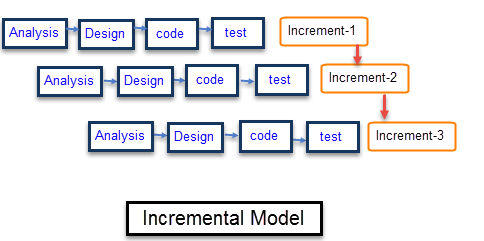
\includegraphics[width=0.85\textwidth]{incremental-model.png}
  \caption{Principe de la méthode incrémentale}
  \label{fig:methode-incrementale-2}
\end{figure}

\subsection{Outils de gestion de projet}

\begin{itemize}
    \item \textbf{Git} — versionnement de l'intégralité des artefacts (pipelines XML, manifestes JSON, code Python/React, skills IA) ;
    \item \textbf{Redmine} — suivi des tickets et des tâches par incrément ;
    \item \textbf{Google Meet} — réunions quotidiennes (daily stand-ups) avec les managers projet et technique.
\end{itemize}

\begin{figure}[H]
  \centering
  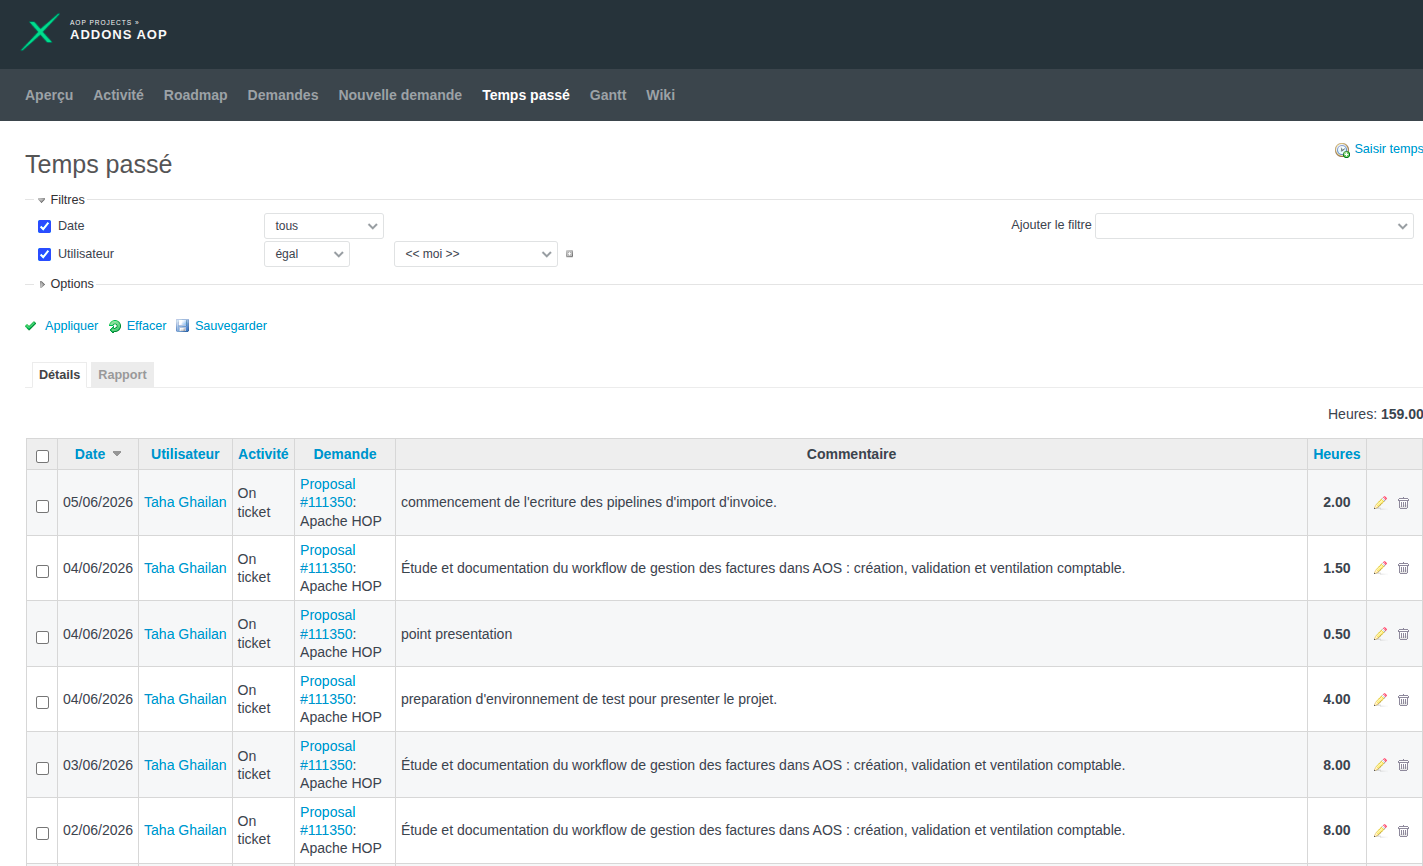
\includegraphics[width=\textwidth]{redmine-tickets.png}
  \caption{Plateforme Redmine — suivi des tickets du projet}
  \label{fig:suivi-redmine}
\end{figure}

\begin{figure}[H]
  \centering
  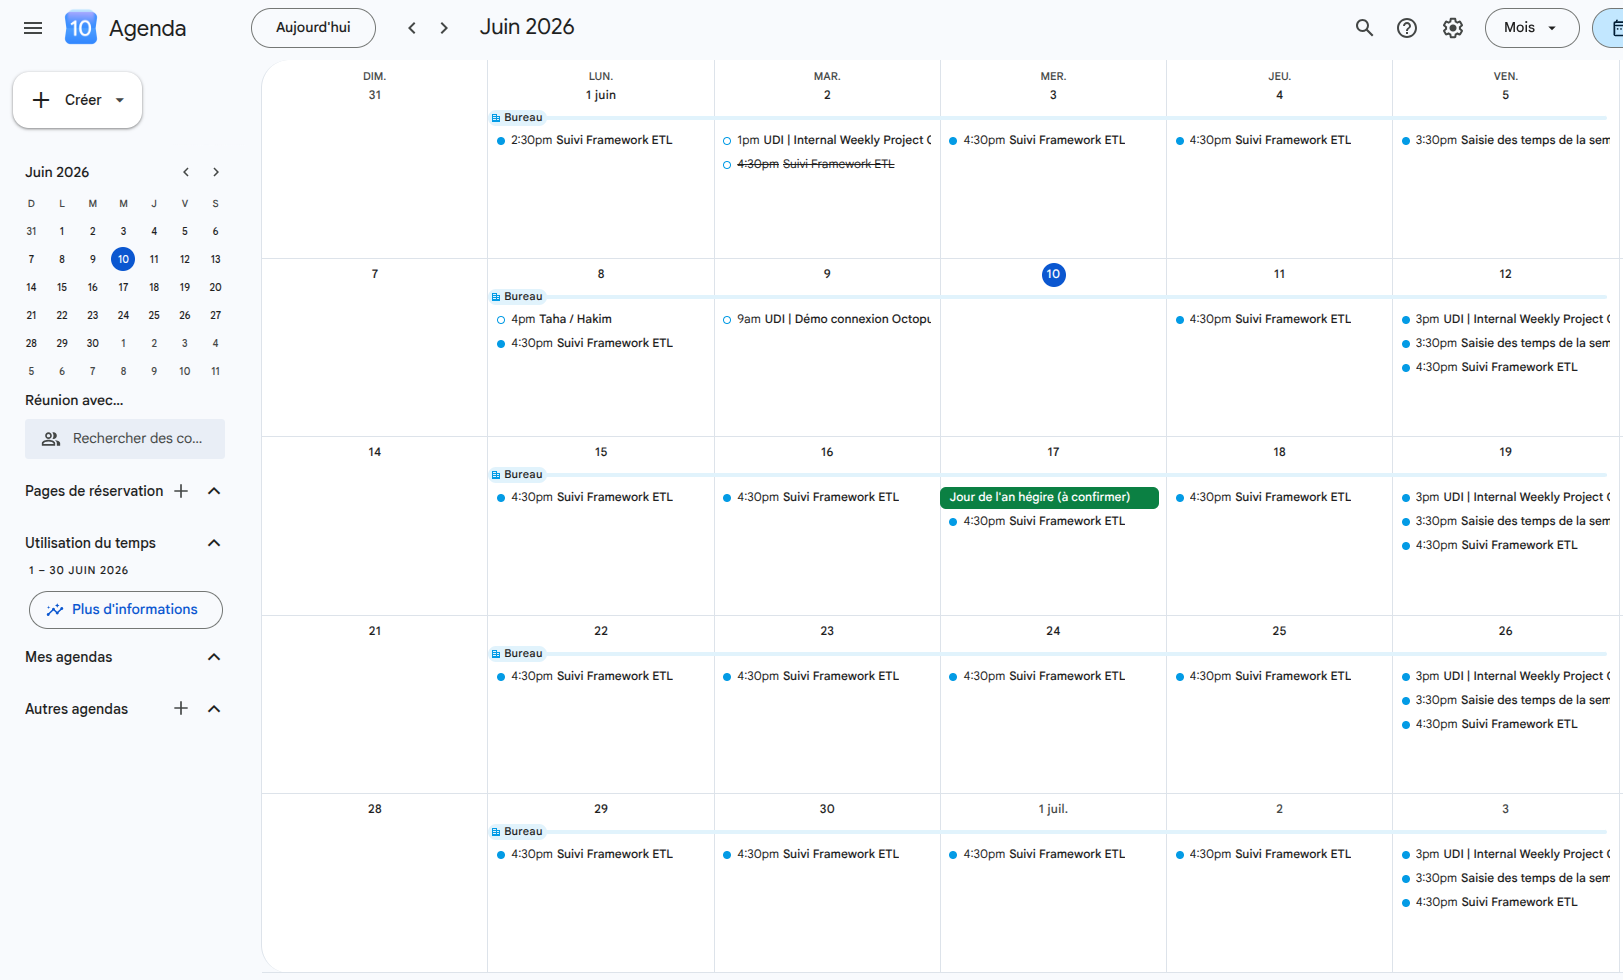
\includegraphics[width=\textwidth]{agenda-google-dailies.png}
  \caption{Extrait de l'agenda Google — réunions quotidiennes de suivi}
  \label{fig:suivi-agenda}
\end{figure}

\subsection{Équipe projet}

L'équipe projet impliquée dans la réalisation de ce stage est présentée dans le tableau~\ref{tab:equipe-projet}.

\begin{table}[H]
  \centering
  \renewcommand{\arraystretch}{1.5}
  \begin{tabular}{p{5cm} p{3.5cm} p{5.5cm}}
    \toprule
    \rowcolor{gray!20}
    \textbf{Nom} & \textbf{Rôle} & \textbf{Fonction} \\
    \midrule
    \rowcolor{gray!5}
    Taha GHAILAN              & Stagiaire PFE       & Conception et développement du framework ETL et de l'application Mapper \\
    M. Abderrahim Aabane      & Tuteur entreprise   & Ingénieur R\&D, Axelor Maroc — encadrement technique quotidien \\
    \rowcolor{gray!5}
    M. Pierre Couderc         & Manager projet      & Pilotage projet et validation des livrables, Axelor \\
    M. Jonathan Michelon      & Manager technique   & Validation des choix d'architecture, Axelor \\
    \rowcolor{gray!5}
    Pr. El Bouzekri El Idrissi Younes & Encadrant académique & Professeur à l'ENSA de Kénitra \\
    \bottomrule
  \end{tabular}
  \caption{Ressources humaines du projet}
  \label{tab:equipe-projet}
\end{table}

\subsection{Incréments réalisés}

Le projet a été découpé en sept incréments~:

\begin{itemize}
  \item \textbf{Incrément 1~:} Pipelines d'import des produits
  \item \textbf{Incrément 2~:} Pipelines d'import des partenaires
  \item \textbf{Incrément 3~:} Pipelines d'import des commandes de vente
  \item \textbf{Incrément 4~:} Pipelines d'import des factures
  \item \textbf{Incrément 5~:} Interface Axelor Mapper
  \item \textbf{Incrément 6~:} Skill analyze-and-map
  \item \textbf{Incrément 7~:} Skills de génération (pipelines + workflows)
\end{itemize}

%% ============================================================
\section{Planification du projet}
\label{sec:planning}
%% ============================================================

\begin{figure}[H]
    \centering
    \begin{ganttchart}[
        hgrid,
        vgrid,
        x unit=0.6cm,
        y unit chart=0.7cm,
        title height=1,
        bar/.style={fill=blue!40},
        bar label font=\small,
        title label font=\small
    ]{1}{15}
        \gantttitle{Semaines}{15} \\
        \gantttitlelist{1,...,15}{1} \\

        \ganttbar{Écriture des pipelines ETL}{1}{4} \\
        \ganttbar{Application Axelor Mapper}{5}{7} \\
        \ganttbar{Écriture des skills IA}{8}{11} \\
        \ganttbar{Tests, validation \& rédaction}{12}{15}
    \end{ganttchart}
    \caption{Diagramme de Gantt — planning de réalisation}
    \label{fig:gantt-2}
\end{figure}

%% ============================================================
\section*{Conclusion}
%% ============================================================

Ce chapitre a formalisé les besoins du framework, présenté la méthodologie incrémentale adoptée, les outils de gestion et le planning de réalisation. Le chapitre suivant présente la conception fonctionnelle du système à travers les diagrammes UML.

\chapter{Conception fonctionnelle}
\label{chap:conception-fonctionnelle}

Ce chapitre a pour but de faire la modélisation du système AOS-ETL à partir de diagrammes UML. On y trouve un diagramme de cas d'utilisation précisant les acteurs principaux et leurs interactions avec le système, des diagrammes de séquence relatant les processus clés, un diagramme de classes destiné à représenter les entités fondamentales et leurs relations.

%% ============================================================
\section{Modélisation du système}
\label{sec:modelisation}
%% ============================================================

\subsection{Définition d'UML}

Le langage de modélisation unifié (UML) est un langage visuel standardisé lequel se prête à spécifier, visualiser, construire et documenter les systèmes logiciels, et permet de comprendre de façon claire la structure et le comportement d'un système, en diminuant les ambiguïtés et en garantissant la cohérence tout au long du projet~\cite{uml}.

\begin{figure}[H]
    \centering
    
\includegraphics[width=0.7\textwidth]{uml.jpeg}
    \caption{Les différents types de diagrammes UML}
    \label{fig:uml-types}
\end{figure}

\subsection{Diagramme de cas d'utilisation}

Le diagramme de cas d'utilisation ci-dessous présente les acteurs du système et leurs interactions principales avec le framework AOS-ETL.

\begin{figure}[H]
    \centering
    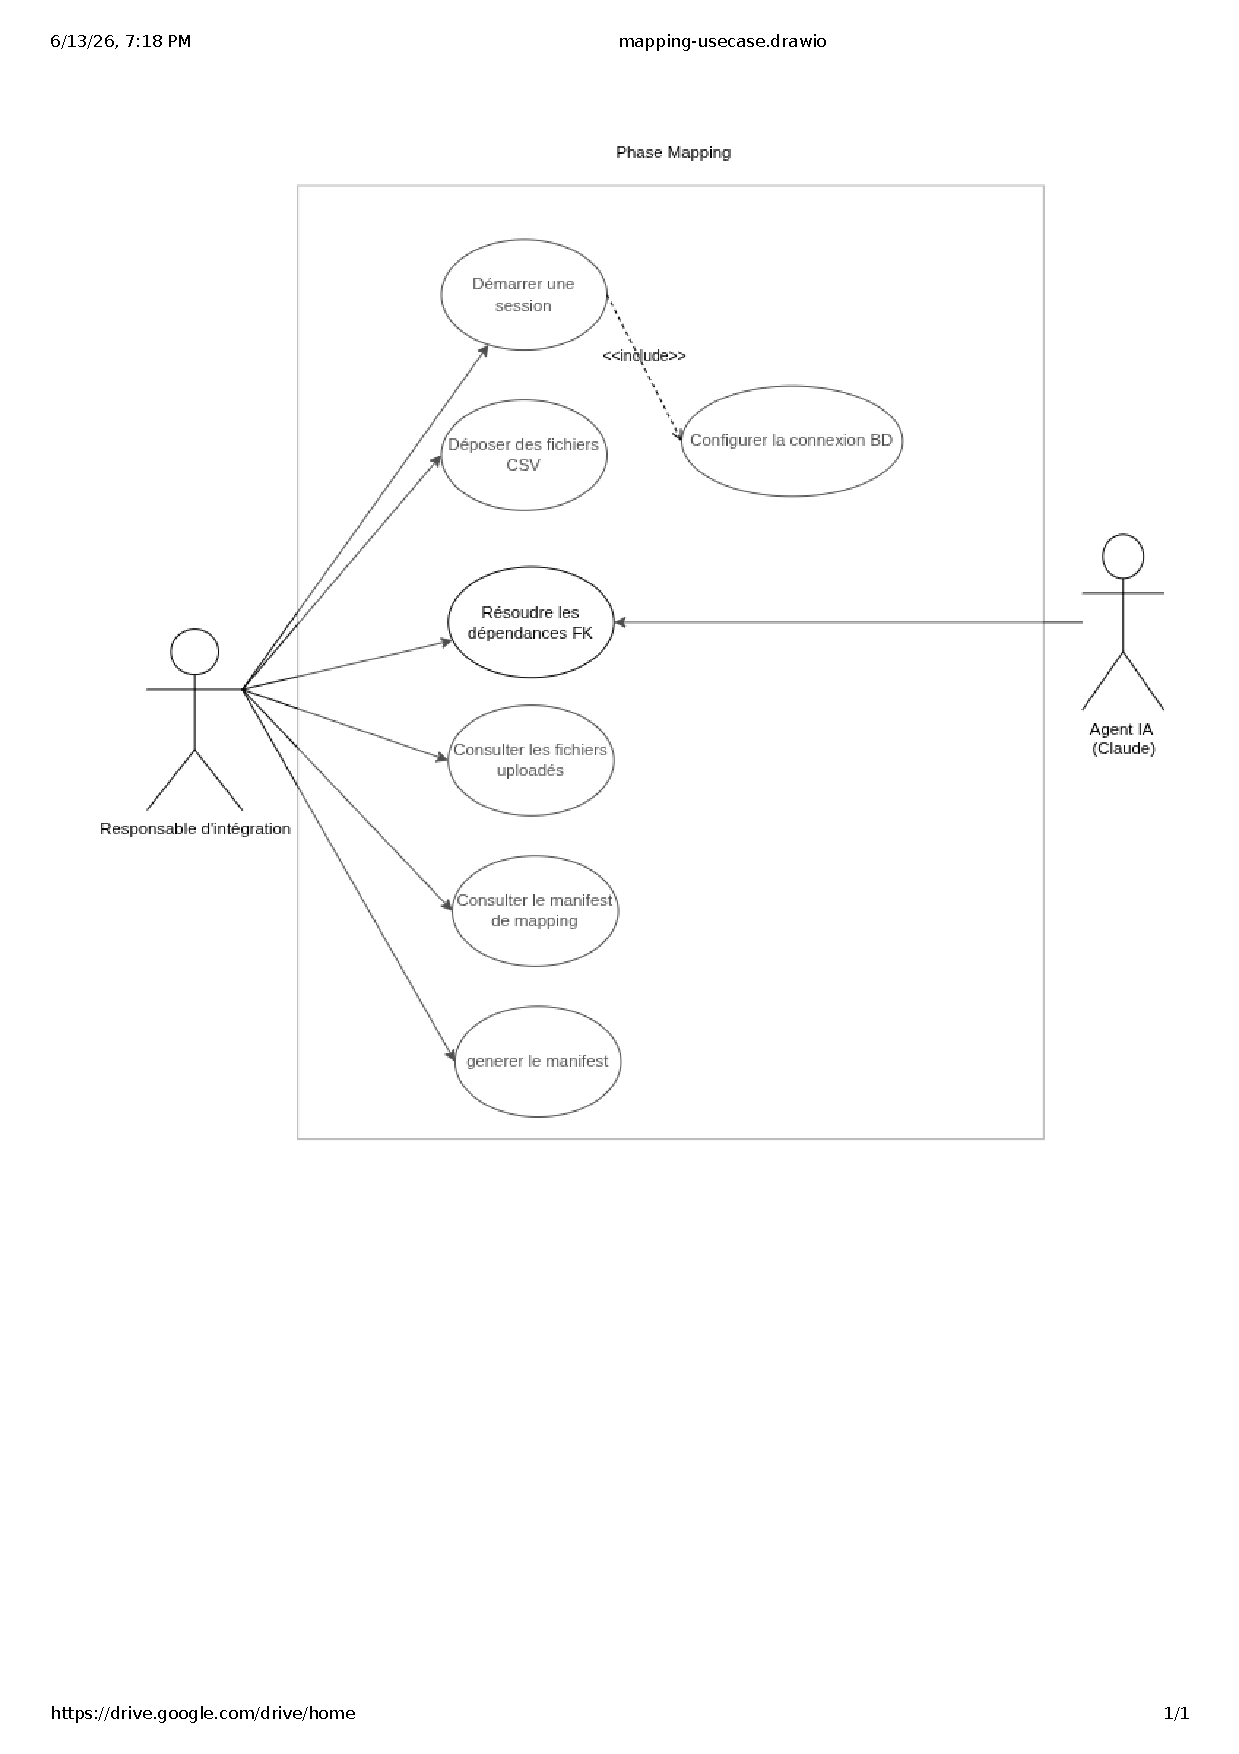
\includegraphics[width=\textwidth, trim=0 240 0 40, clip]{phase-mapping-use-case.pdf}
    \caption{Diagramme de cas d'utilisation — Phase Mapping}
    \label{fig:use-case-mapping}
\end{figure}

\begin{figure}[H]
    \centering
    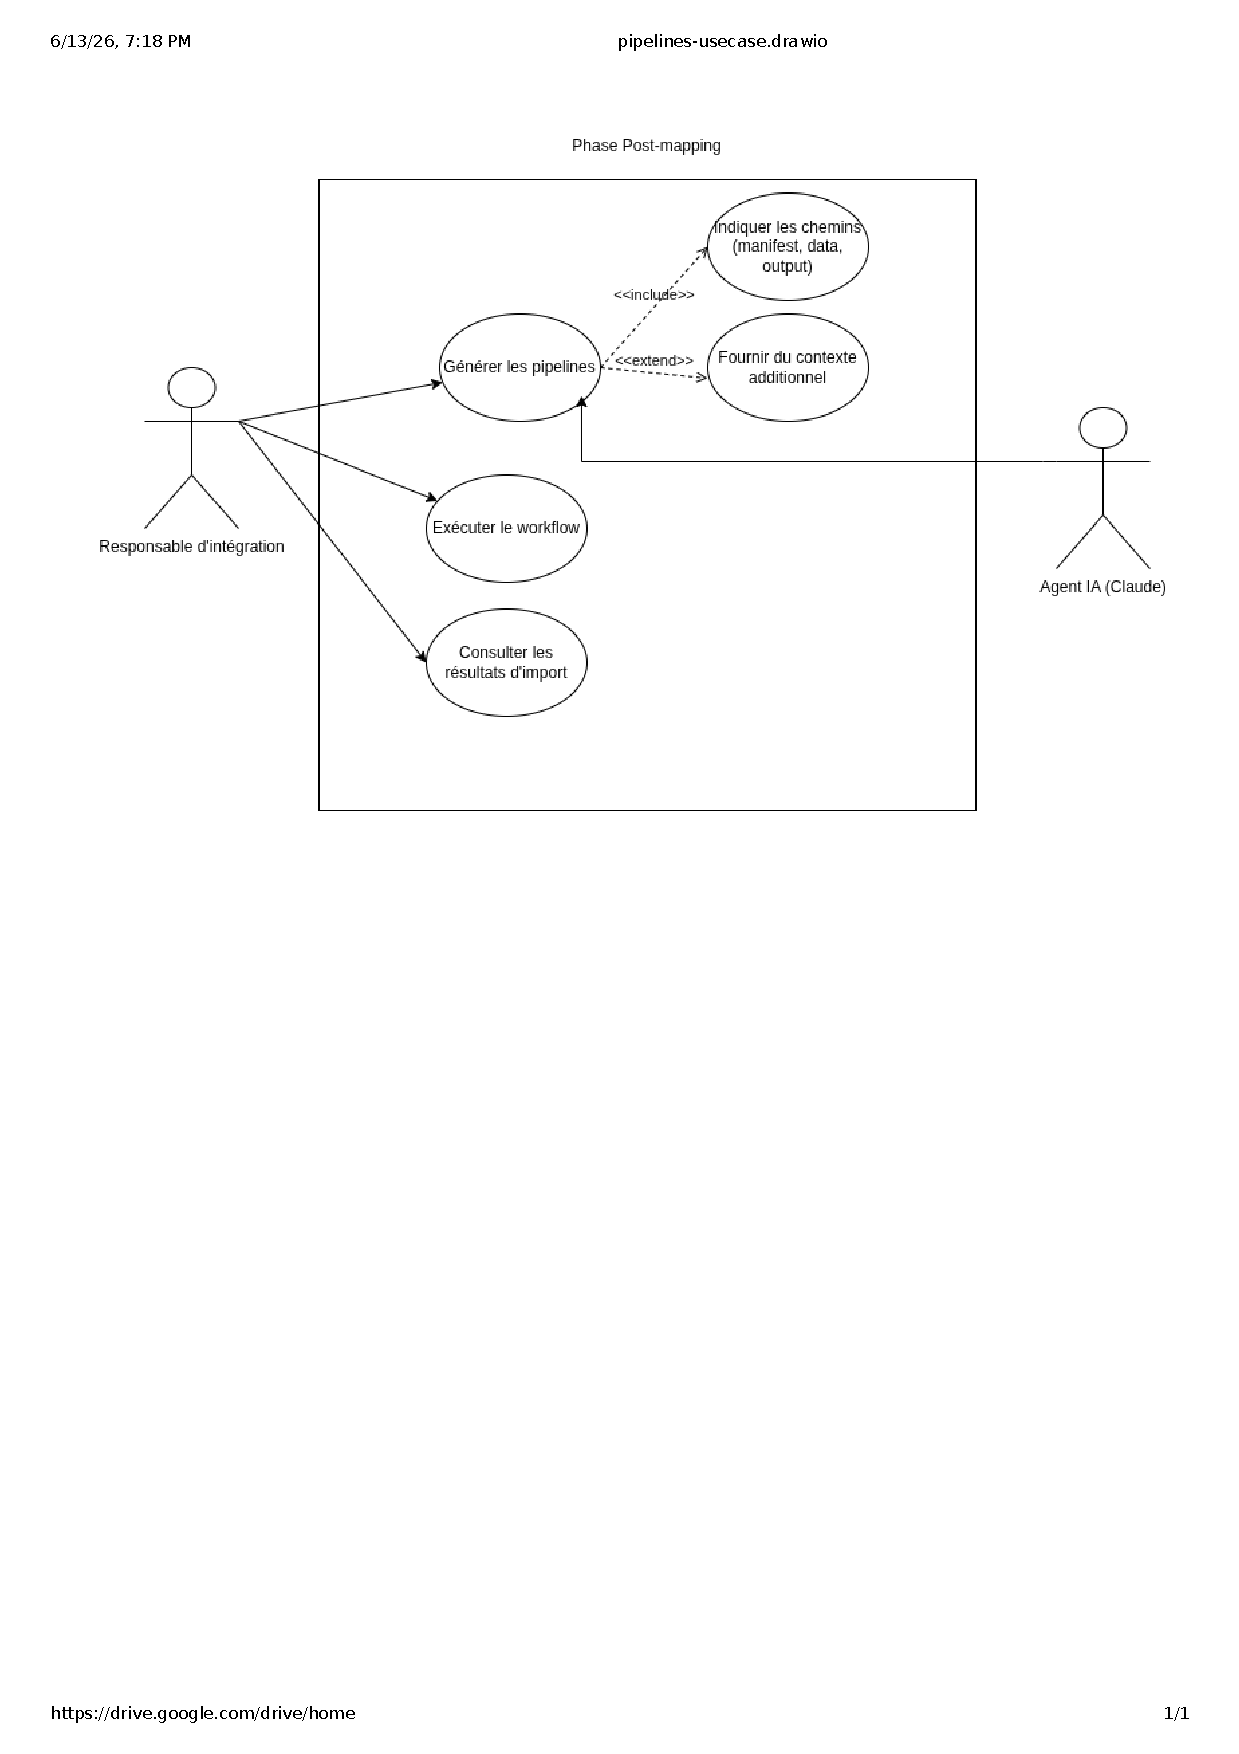
\includegraphics[width=\textwidth, trim=0 400 0 40, clip]{post-mapping-use-case.pdf}
    \caption{Diagramme de cas d'utilisation — Phase Post-mapping}
    \label{fig:use-case-post-mapping}
\end{figure}

Les acteurs identifiés sont~:
\begin{itemize}
    \item \textbf{Responsable d'intégration~:} utilisateur principal qui upload les fichiers CSV, interagit avec l'agent de mapping, lance la génération des pipelines et l'exécution des imports ;
    \item \textbf{Agent IA (Claude)~:} acteur secondaire qui analyse les CSV, résout les dépendances FK, génère les manifestes et les pipelines.
\end{itemize}

\subsection{Raffinement des cas d'utilisation}

Le tableau~\ref{tab:raffinement} détaille les actions possibles par acteur.

\begin{table}[H]
  \centering
  \renewcommand{\arraystretch}{1.4}
  \begin{tabular}{p{3.5cm} p{4cm} p{6cm}}
    \toprule
    \rowcolor{gray!20}
    \textbf{Acteur} & \textbf{Action} & \textbf{Description} \\
    \midrule
    \rowcolor{gray!5}
    Responsable d'intégration & Démarrer une session & Choisit l'entité cible et configure la connexion BD \\
    Responsable d'intégration & Déposer des fichiers CSV & Upload un ou plusieurs fichiers dans la session \\
    \rowcolor{gray!5}
    Responsable d'intégration & Résoudre les FK & Répond aux questions de l'agent sur les ambiguïtés \\
    Responsable d'intégration & Consulter les fichiers & Vérifie les fichiers déposés dans la session \\
    \rowcolor{gray!5}
    Responsable d'intégration & Consulter le manifest & Revue du mapping proposé par l'agent \\
    Responsable d'intégration & Générer les pipelines & Lance la génération avec paramètres (paths, contexte) \\
    \rowcolor{gray!5}
    Responsable d'intégration & Exécuter le workflow & Lance l'import via hop-run.sh \\
    Responsable d'intégration & Consulter les résultats & Vérifie les lignes importées et les erreurs \\
    \midrule
    \rowcolor{gray!5}
    Agent IA (Claude) & Analyser le CSV & Profile les colonnes, détecte les types et FK \\
    Agent IA (Claude) & Résoudre les FK & Vérifie en BD l'existence des valeurs référencées \\
    \rowcolor{gray!5}
    Agent IA (Claude) & Produire le manifest & Écrit le fichier manifest.json \\
    Agent IA (Claude) & Générer les pipelines & Produit les fichiers .hpl/.hwf \\
    \bottomrule
  \end{tabular}
  \caption{Raffinement des cas d'utilisation}
  \label{tab:raffinement}
\end{table}

\subsection{Diagrammes de séquence}

\subsubsection{Séquence — Phase Mapping}

\begin{figure}[H]
    \makebox[\textwidth][c]{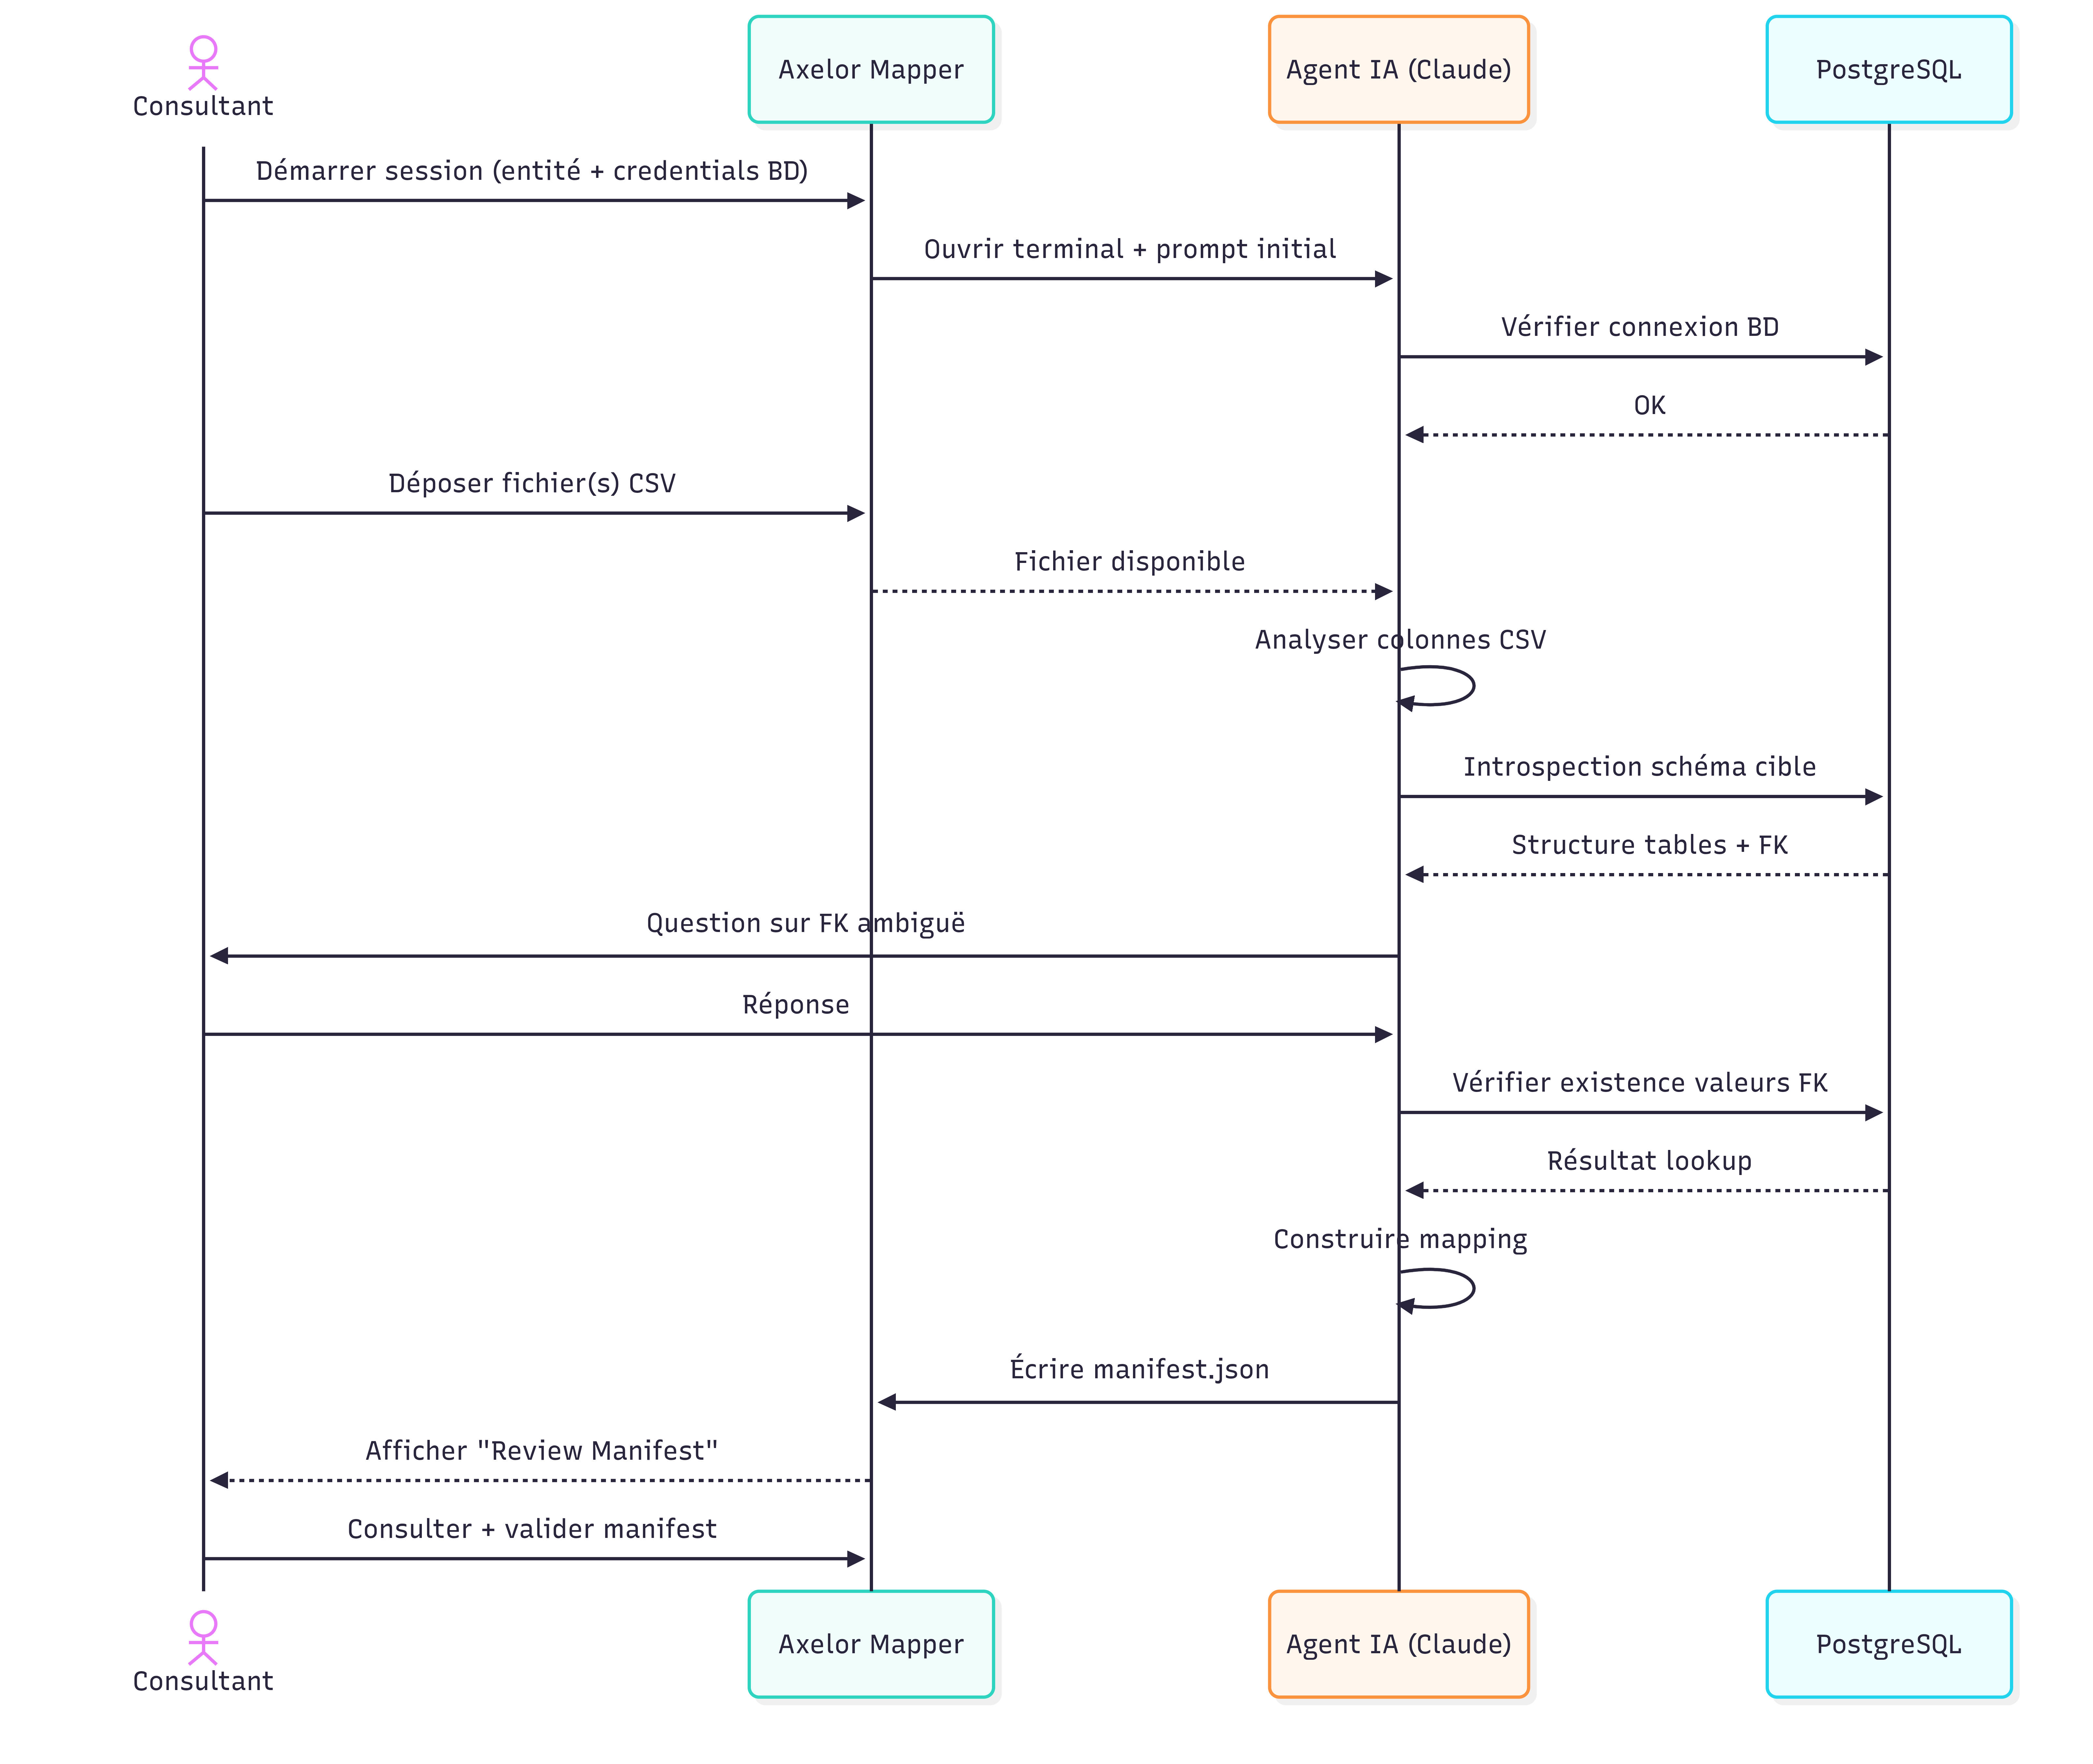
\includegraphics[width=1.25\textwidth]{uml-sequence-mapping.png}}
    \caption{Diagramme de séquence — session de mapping via l'agent IA}
    \label{fig:seq-mapping}
\end{figure}

\clearpage

\subsubsection{Séquence — Phase Post-mapping}

\begin{figure}[H]
    \makebox[\textwidth][c]{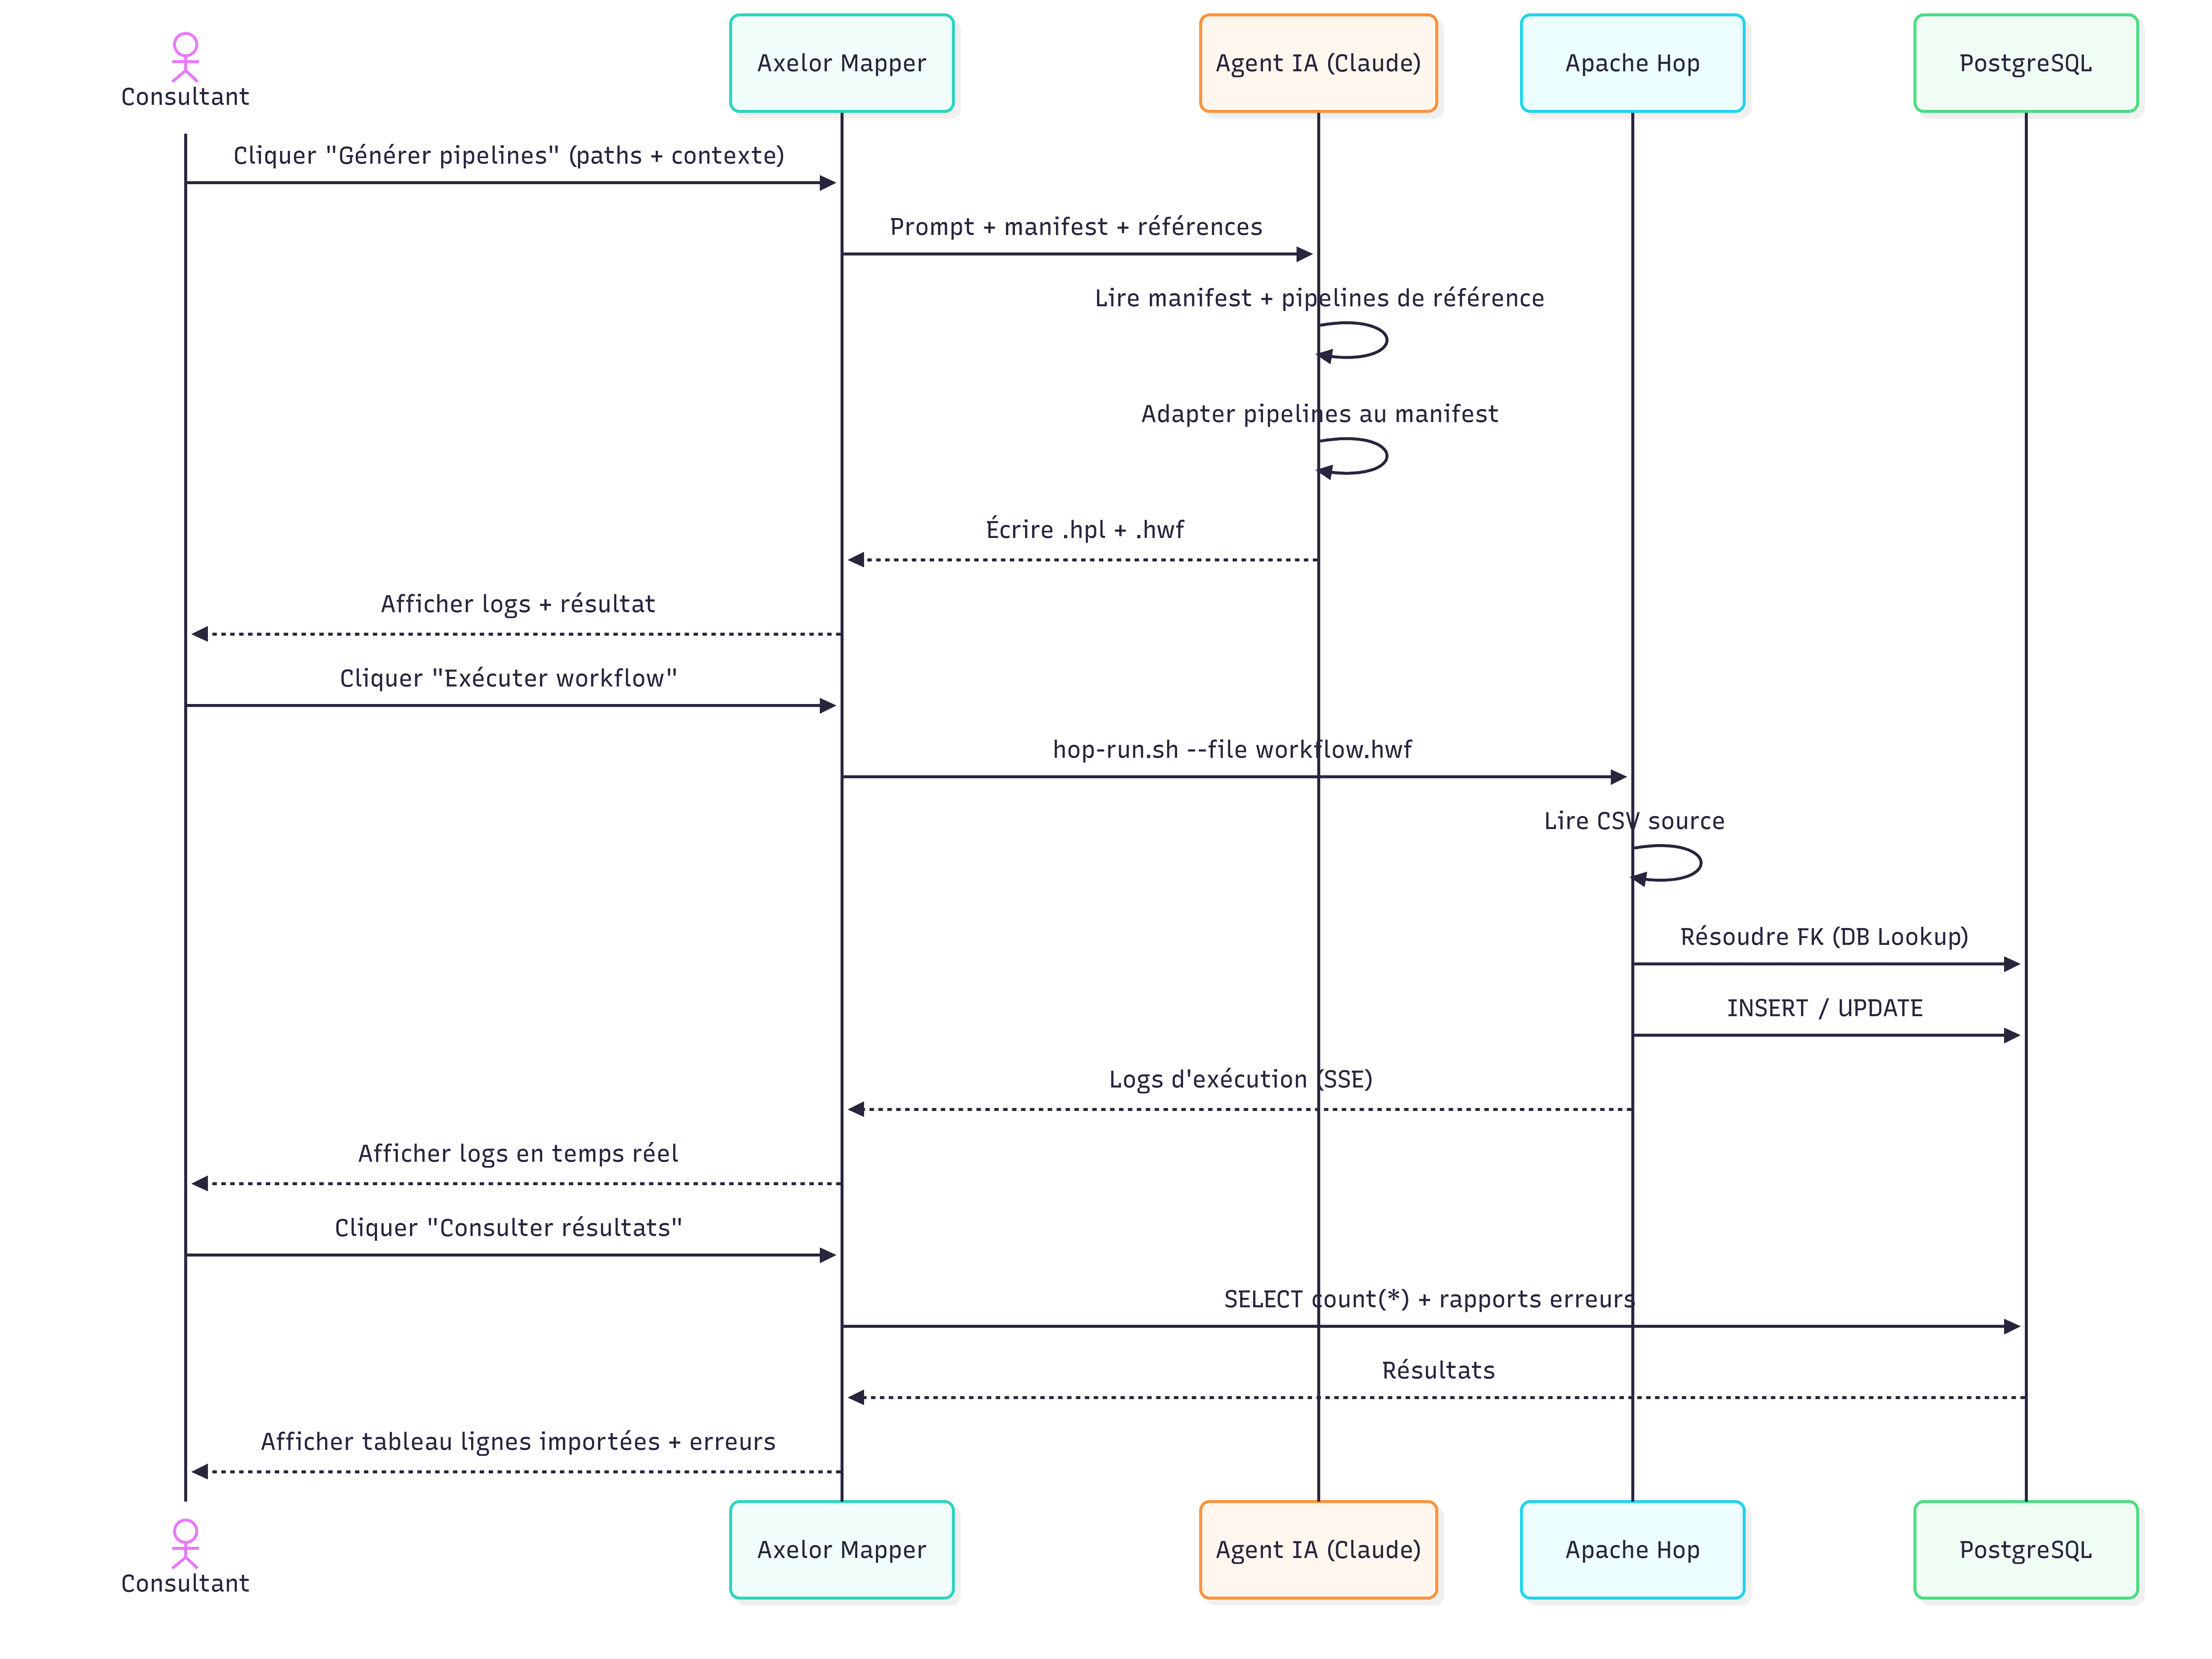
\includegraphics[width=1.25\textwidth]{uml-sequence-postmapping.png}}
    \caption{Diagramme de séquence — génération et exécution des pipelines}
    \label{fig:seq-postmapping}
\end{figure}

\clearpage

\subsection{Diagramme de classes}

\begin{figure}[H]
    \centering
    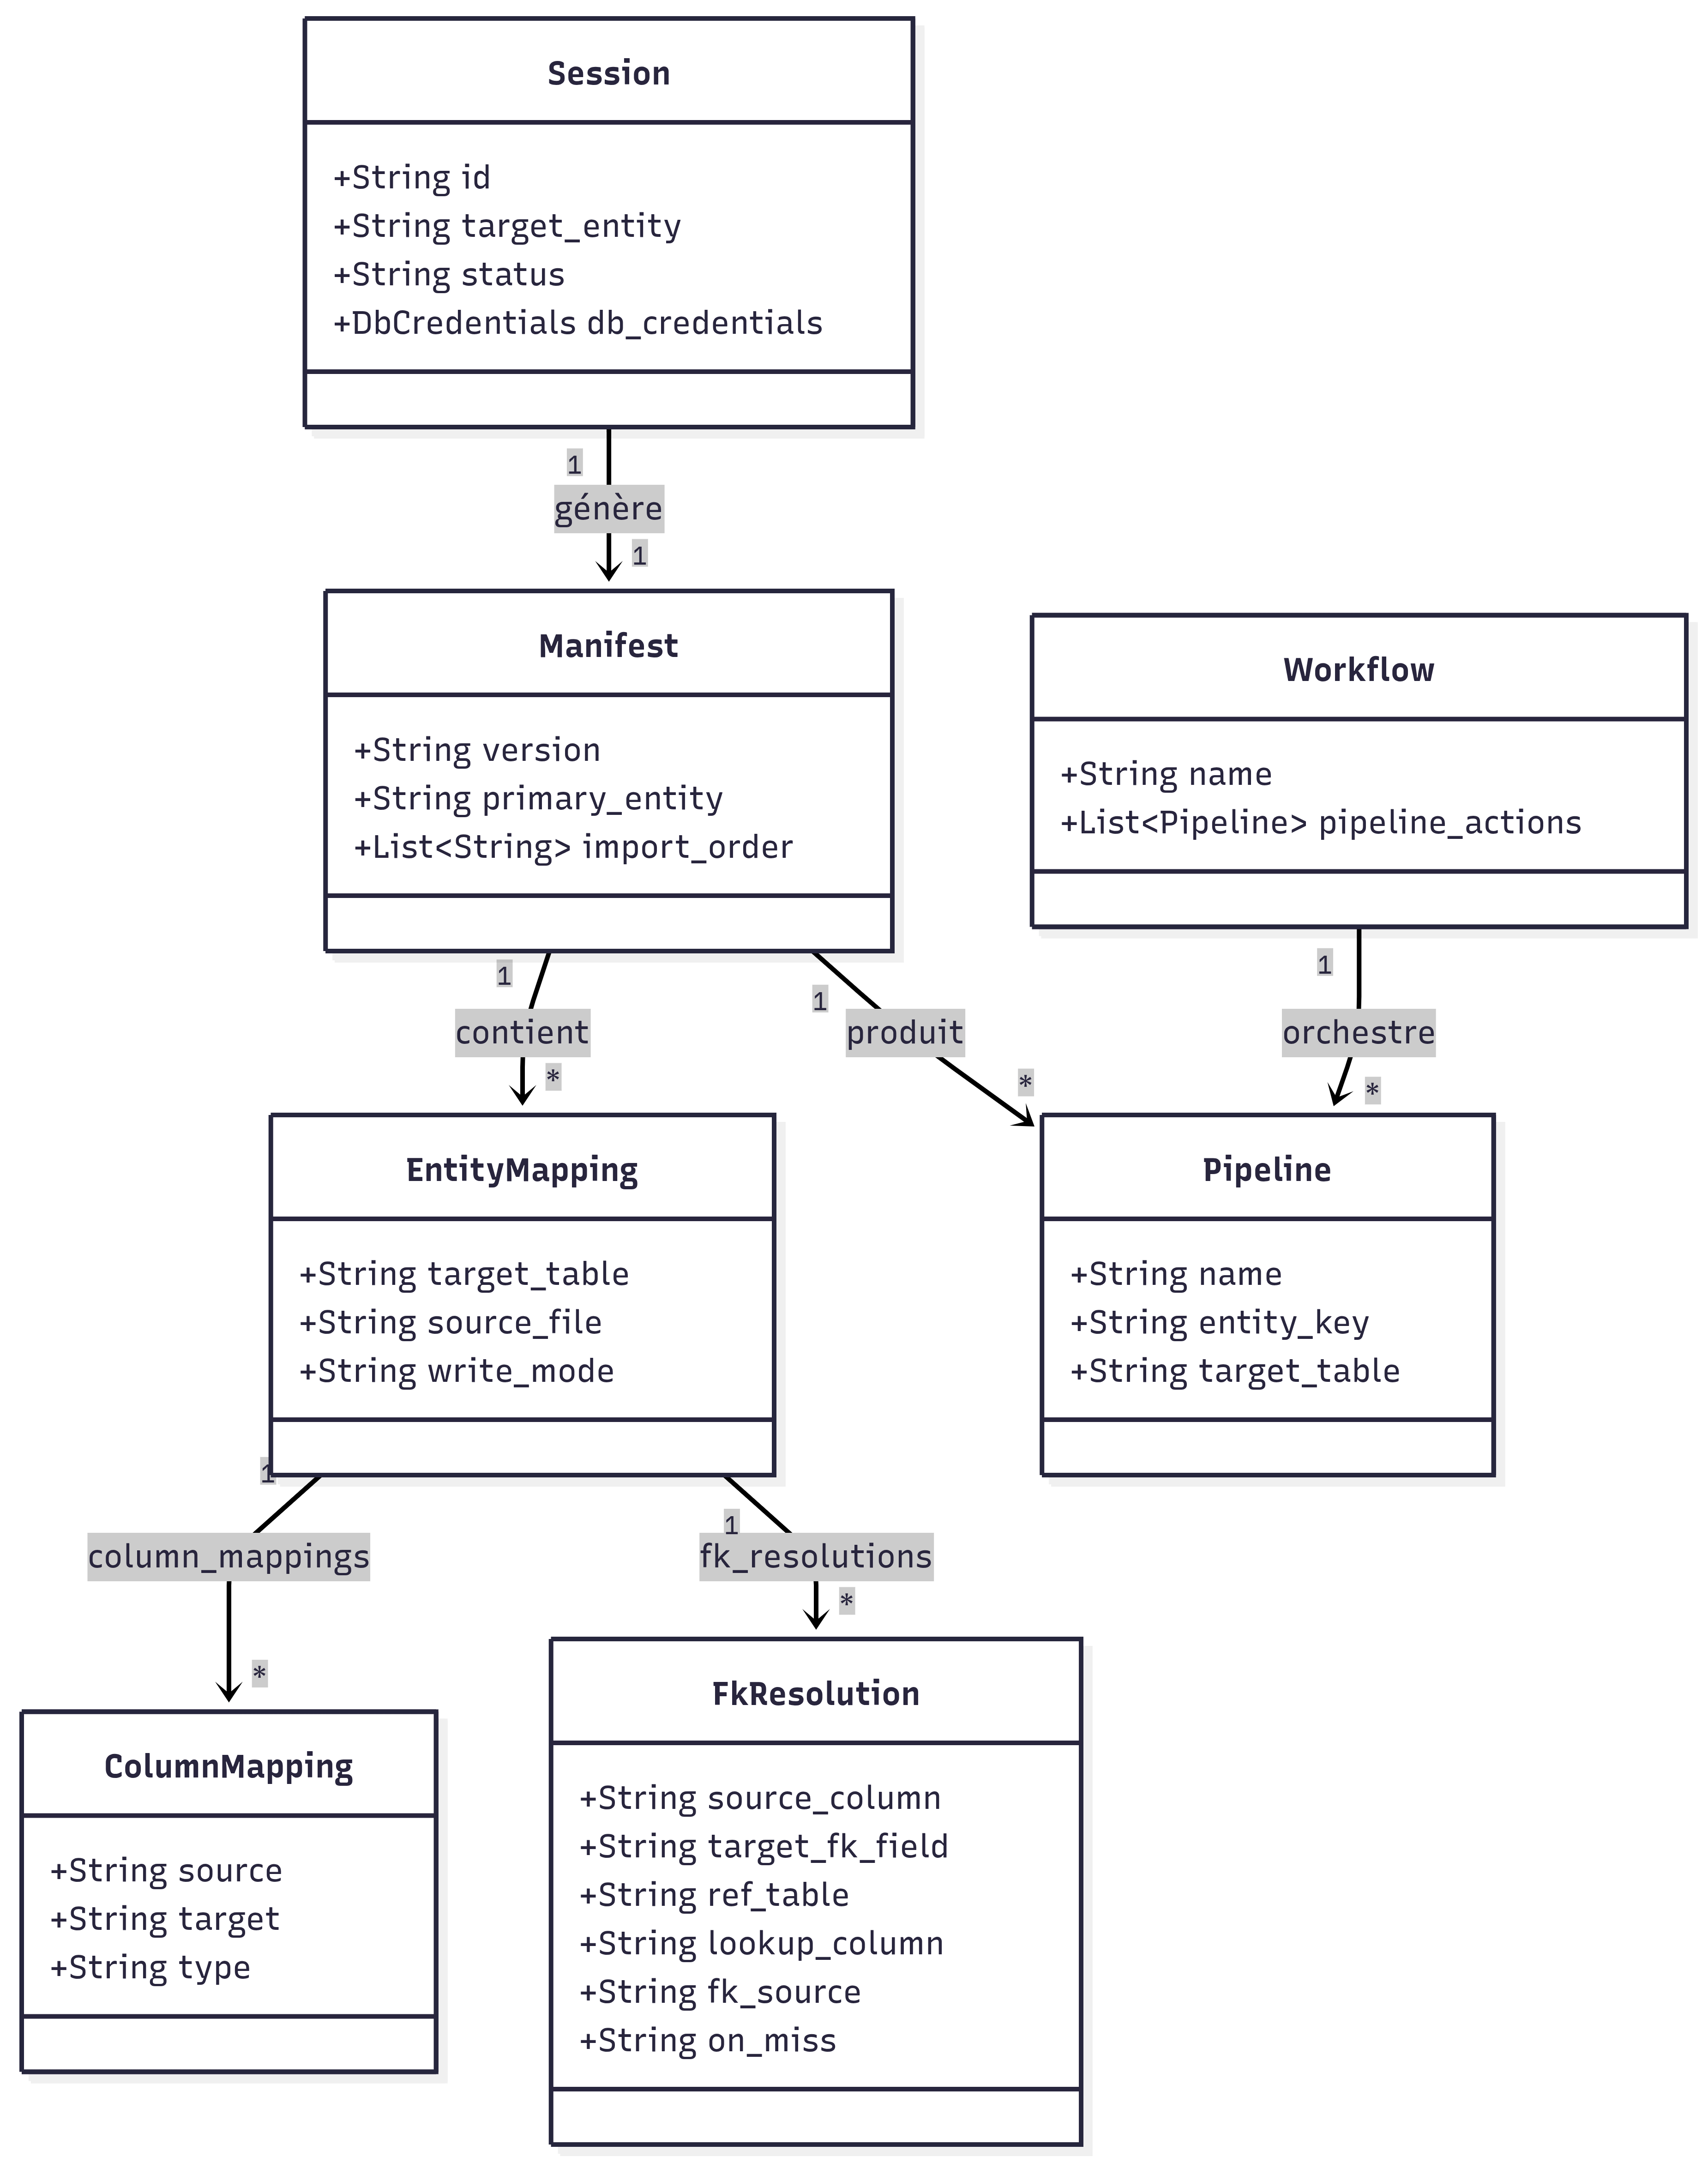
\includegraphics[width=0.9\textwidth]{uml-class-diagram.png}
    \caption{Diagramme de classes du framework AOS-ETL}
    \label{fig:class-diagram}
\end{figure}

%% ============================================================
\section*{Conclusion}
%% ============================================================

Ce chapitre a offert une vue fonctionnelle du système au moyen de diagrammes UML. Les cas d'utilisation ont permis de repérer les interactions entre le responsable d'intégration et le système, les diagrammes de séquence ont détaillé les flux principaux et le diagramme de classes a formalisé les entités majeures du framework. Le chapitre suivant explique l'architecture technique de la solution.

\chapter{Architecture technique}
\label{chap:architecture}

Ce chapitre présente les choix technologiques effectués, l'architecture globale de la solution et les mesures de sécurité adoptées.

%% ============================================================
\section{Benchmark des technologies}
\label{sec:benchmark}
%% ============================================================

Cette section présente les études comparatives réalisées pour justifier les choix technologiques du framework.

\subsection{Outil ETL}

Le choix de l'outil ETL est déterminant car il conditionne la manière dont les pipelines d'import sont conçus, maintenus et — dans notre cas — générés automatiquement par IA. Les processus ETL constituent un domaine central des architectures d'intégration de données~\cite{vassiliadis2009}. Trois alternatives ont été évaluées :

\begin{itemize}
    \item \textbf{Apache Hop} — plateforme ETL open source (licence Apache 2.0), fork modernisé de Kettle créé en 2020 par ses auteurs originaux. Les pipelines sont définis en fichiers XML (\texttt{.hpl}), exécutables en ligne de commande via \texttt{hop-run.sh}.
    \item \textbf{Talend Open Studio} — outil ETL en modèle freemium. L'interface graphique génère du code Java compilé (.jar). Le versionnement est complexe car chaque modification regenere l'intégralité du code source.
    \item \textbf{Apache NiFi} — plateforme de data flow temps réel, conçue pour le routage et la distribution de données en streaming (Kafka, IoT, API). Fonctionne comme un serveur web permanent avec une interface de configuration.
\end{itemize}

Les critères de comparaison retenus sont les suivants :

\begin{itemize}
    \item \textbf{Format des pipelines~:} le format dans lequel les pipelines sont stockés sur disque. Un format texte structuré (XML) est essentiel pour notre projet car il permet la génération automatique par un LLM et le versionnement ligne par ligne dans Git.
    \item \textbf{Généreable par LLM~:} la capacité d'un modèle de langage à produire un pipeline valide à partir d'instructions. Nécessite un format texte lisible avec une structure prévisible.
    \item \textbf{Pattern upsert natif~:} la disponibilité d'un composant intégré qui vérifie l'existence d'un enregistrement avant de décider entre INSERT et UPDATE — sans nécessiter de scripting custom.
    \item \textbf{Exécution CLI sans serveur~:} la possibilité d'exécuter un pipeline en une commande terminal, sans qu'un serveur doive tourner en permanence.
    \item \textbf{Licence~:} la compatibilité avec l'écosystème open source d'Axelor (AGPLv3).
\end{itemize}

\begin{table}[H]
  \centering
  \renewcommand{\arraystretch}{1.4}
  \begin{tabular}{p{3.5cm} p{3.2cm} p{3.2cm} p{3.2cm}}
    \toprule
    \rowcolor{gray!20}
    \textbf{Critère} & \textbf{Apache Hop} & \textbf{Talend} & \textbf{Apache NiFi} \\
    \midrule
    \rowcolor{gray!5}
    Format des pipelines & XML lisible (\texttt{.hpl}) & Java compilé (.jar) & JSON interne (binaire) \\
    Généreable par LLM   & Oui              & Non                & Non \\
    \rowcolor{gray!5}
    Pattern upsert natif & Oui (Insert/Update) & Oui (tMap)      & Non (scripting requis) \\
    Exécution CLI        & Oui (\texttt{hop-run.sh}) & Oui (jar)  & Non (serveur web) \\
    \rowcolor{gray!5}
    Versionnement Git    & Natif (1 fichier = 1 pipeline) & Complexe (regenere tout) & Difficile (JSON imbriqué) \\
    Licence              & Apache 2.0       & Freemium           & Apache 2.0 \\
    \bottomrule
  \end{tabular}
  \caption{Comparaison des outils ETL (sources~: documentation officielle Apache Hop~\cite{hop-doc}, Talend~\cite{talend-doc}, Apache NiFi~\cite{nifi-doc})}
  \label{tab:benchmark-etl}
\end{table}

\textbf{Choix retenu~:} Apache Hop. Le critère déterminant est la \textbf{générabilité par LLM}~: les pipelines étant des fichiers XML avec une structure prévisible, un agent IA peut les lire comme contexte et en produire de nouveaux. Aucune autre solution ne permet cela — Talend génère du bytecode Java inexploitable, et NiFi stocke sa configuration dans un format interne non conçu pour la production programmatique. De plus, Hop offre nativement le pattern upsert (composant Insert/Update) et l'exécution en ligne de commande, deux prérequis de notre architecture.

\subsection{Agent IA de génération de code}

Le framework nécessite un agent IA capable de générer du code structuré (XML Apache Hop, JSON) à partir d'instructions en langage naturel. Les grands modèles de langage ont démontré leur capacité à générer du code à partir d'exemples~\cite{brown2020}, ouvrant la voie à des agents d'assistance au développement~\cite{chen2023}. En 2025-2026, trois agents de code en terminal sont disponibles :

\begin{itemize}
    \item \textbf{Claude Code (Anthropic)} — CLI avec système de \textit{slash commands} intégré (fichiers \texttt{.md} dans \texttt{.claude/commands/}) permettant de structurer les prompts en skills modulaires. Supporte le prompt caching~\cite{anthropic_claude}.
    \item \textbf{Codex CLI (OpenAI)} — agent open source (MIT), basé sur GPT-5.5. Exécution locale en terminal~\cite{openai_codex}.
    \item \textbf{Gemini CLI (Google)} — agent open source (Apache 2.0), basé sur Gemini 3.1 Pro. Accès gratuit (1000 requêtes/jour)~\cite{google_gemini_cli}.
\end{itemize}

Le tableau~\ref{tab:benchmark-ia} présente une comparaison basée sur les benchmarks indépendants d'Artificial Analysis (juin 2026).

\begin{table}[H]
  \centering
  \renewcommand{\arraystretch}{1.4}
  \begin{tabular}{p{3.5cm} p{3cm} p{3cm} p{3cm}}
    \toprule
    \rowcolor{gray!20}
    \textbf{Critère} & \textbf{Claude Code} & \textbf{Codex CLI} & \textbf{Gemini CLI} \\
    \midrule
    \rowcolor{gray!5}
    Coding Agent Index  & 77              & 76                & — \\
    Terminal-Bench Hard & 63\%            & 61\%              & 54\% \\
    \rowcolor{gray!5}
    Intelligence Index  & 65              & 60                & 57 \\
    Prix (USD/1M tokens) & 7.7            & 4.3               & 1.7 \\
    \rowcolor{gray!5}
    Contexte max (tokens) & 200K--1M      & 128K--1M          & 1M \\
    \bottomrule
  \end{tabular}
  \caption{Comparaison des agents IA de code (source~: Artificial Analysis, juin 2026~\cite{artificial-analysis})}
  \label{tab:benchmark-ia}
\end{table}

\textbf{Constat~:} Les trois agents affichent des performances très proches sur les benchmarks de code agentic (77 vs 76 pour Claude Code et Codex). Aucun ne se démarque de manière décisive sur la qualité de génération.

\textbf{Choix retenu~:} Claude Code. Les trois agents étant comparables en performance, le choix s'est fait sur un critère pragmatique~: l'entreprise disposait déjà d'un abonnement Anthropic actif et d'une familiarité avec l'écosystème Claude au moment du démarrage du projet.

\subsection{Stack applicative}

\begin{table}[H]
  \centering
  \renewcommand{\arraystretch}{1.4}
  \begin{tabular}{p{3cm} p{4cm} p{6cm}}
    \toprule
    \rowcolor{gray!20}
    \textbf{Composant} & \textbf{Technologie} & \textbf{Justification} \\
    \midrule
    \rowcolor{gray!5}
    Backend   & FastAPI (Python)        & Prototypage rapide, manipulation CLI/subprocess native \\
    Frontend  & React + TypeScript      & Écosystème riche, xterm.js pour le terminal \\
    \rowcolor{gray!5}
    Terminal  & xterm.js + WebSocket    & Émulation PTY dans le navigateur \\
    Base de données & PostgreSQL        & Imposé par Axelor Open Suite \\
    \rowcolor{gray!5}
    ETL Engine & Apache Hop 2.x        & Pipelines XML déclaratifs \\
    Agent IA  & Claude CLI (Anthropic)  & Abonnement existant en entreprise \\
    \bottomrule
  \end{tabular}
  \caption{Stack technique retenue}
  \label{tab:stack-technique}
\end{table}

\textbf{Backend (FastAPI/Python)~:} Python a été retenu car le backend doit principalement orchestrer des appels CLI (lancer Claude via \texttt{subprocess}, spawner des PTY, exécuter \texttt{hop-run.sh}). Python offre une manipulation native des processus système et un prototypage rapide adapté à un projet de recherche~\cite{fastapi_doc}.

\textbf{Frontend (React + xterm.js)~:} Le choix de React~\cite{react_doc} n'est pas motivé par une contrainte technique particulière — tout framework frontend moderne aurait convenu. La bibliothèque xterm.js~\cite{xtermjs}, utilisée pour l'émulation du terminal dans le navigateur via une communication WebSocket~\cite{websocket_rfc}, est indépendante du framework.

\textbf{PostgreSQL~:} Imposé par Axelor Open Suite — c'est la seule base supportée par l'ERP. Il n'y a pas de choix à faire ici.

%% ============================================================
\section{Architecture globale de la solution}
\label{sec:archi-globale}
%% ============================================================

Le framework suit un flux linéaire allant du fichier CSV source jusqu'à l'insertion en base de données~:

\begin{center}
\textbf{CSV} $\longrightarrow$ \textbf{Agent IA} (analyse + manifest) $\longrightarrow$ \textbf{Agent IA} (génération pipelines) $\longrightarrow$ \textbf{Apache Hop} (exécution) $\longrightarrow$ \textbf{PostgreSQL}
\end{center}

Le processus se décompose en trois étapes principales~:

\begin{enumerate}
    \item \textbf{Analyse et mapping~:} le consultant upload un CSV dans l'application Mapper. L'agent IA analyse la structure du fichier, identifie les colonnes, résout les dépendances FK en interrogeant la base cible, et produit un \textbf{manifeste JSON} décrivant le mapping complet.
    \item \textbf{Génération des pipelines~:} à partir du manifeste, l'agent IA génère les fichiers XML Apache Hop (.hpl) en s'appuyant sur des pipelines de référence existants comme modèles.
    \item \textbf{Exécution~:} les pipelines générés sont exécutés par le moteur Apache Hop via \texttt{hop-run.sh}, qui lit le CSV, applique les transformations et insère les données dans PostgreSQL.
\end{enumerate}

\subsection{Le manifeste JSON comme artefact intermédiaire}

Le manifeste JSON est un fichier qui persiste sur disque entre l'étape d'analyse et l'étape de génération. Il formalise~: la table cible, le mapping des colonnes, les stratégies de résolution FK, l'ordre d'import des entités et les métadonnées de transformation. Cette matérialisation permet de~:
\begin{itemize}
    \item Valider le mapping avec le consultant avant de générer les pipelines ;
    \item Versionner le résultat de l'analyse sous Git ;
    \item Régénérer les pipelines sans relancer l'analyse si seul le format de sortie change.
\end{itemize}

\subsection{Composants du système}

\begin{itemize}
    \item \textbf{Application Axelor Mapper~:} interface web (React + FastAPI) offrant un terminal conversationnel et des actions post-mapping (génération, exécution, consultation des résultats).
    \item \textbf{Skills IA~:} prompts structurés guidant l'agent à travers l'analyse du CSV et la génération des pipelines.
    \item \textbf{Manifeste JSON~:} fichier décrivant le mapping complet d'une entité.
    \item \textbf{Pipelines Apache Hop~:} fichiers XML (.hpl) implémentant les patterns d'import (upsert, insert-only, junction, post-SQL).
    \item \textbf{Workflows Apache Hop~:} fichiers XML (.hwf) orchestrant l'exécution séquentielle des pipelines.
\end{itemize}

\begin{figure}[H]
    \centering
    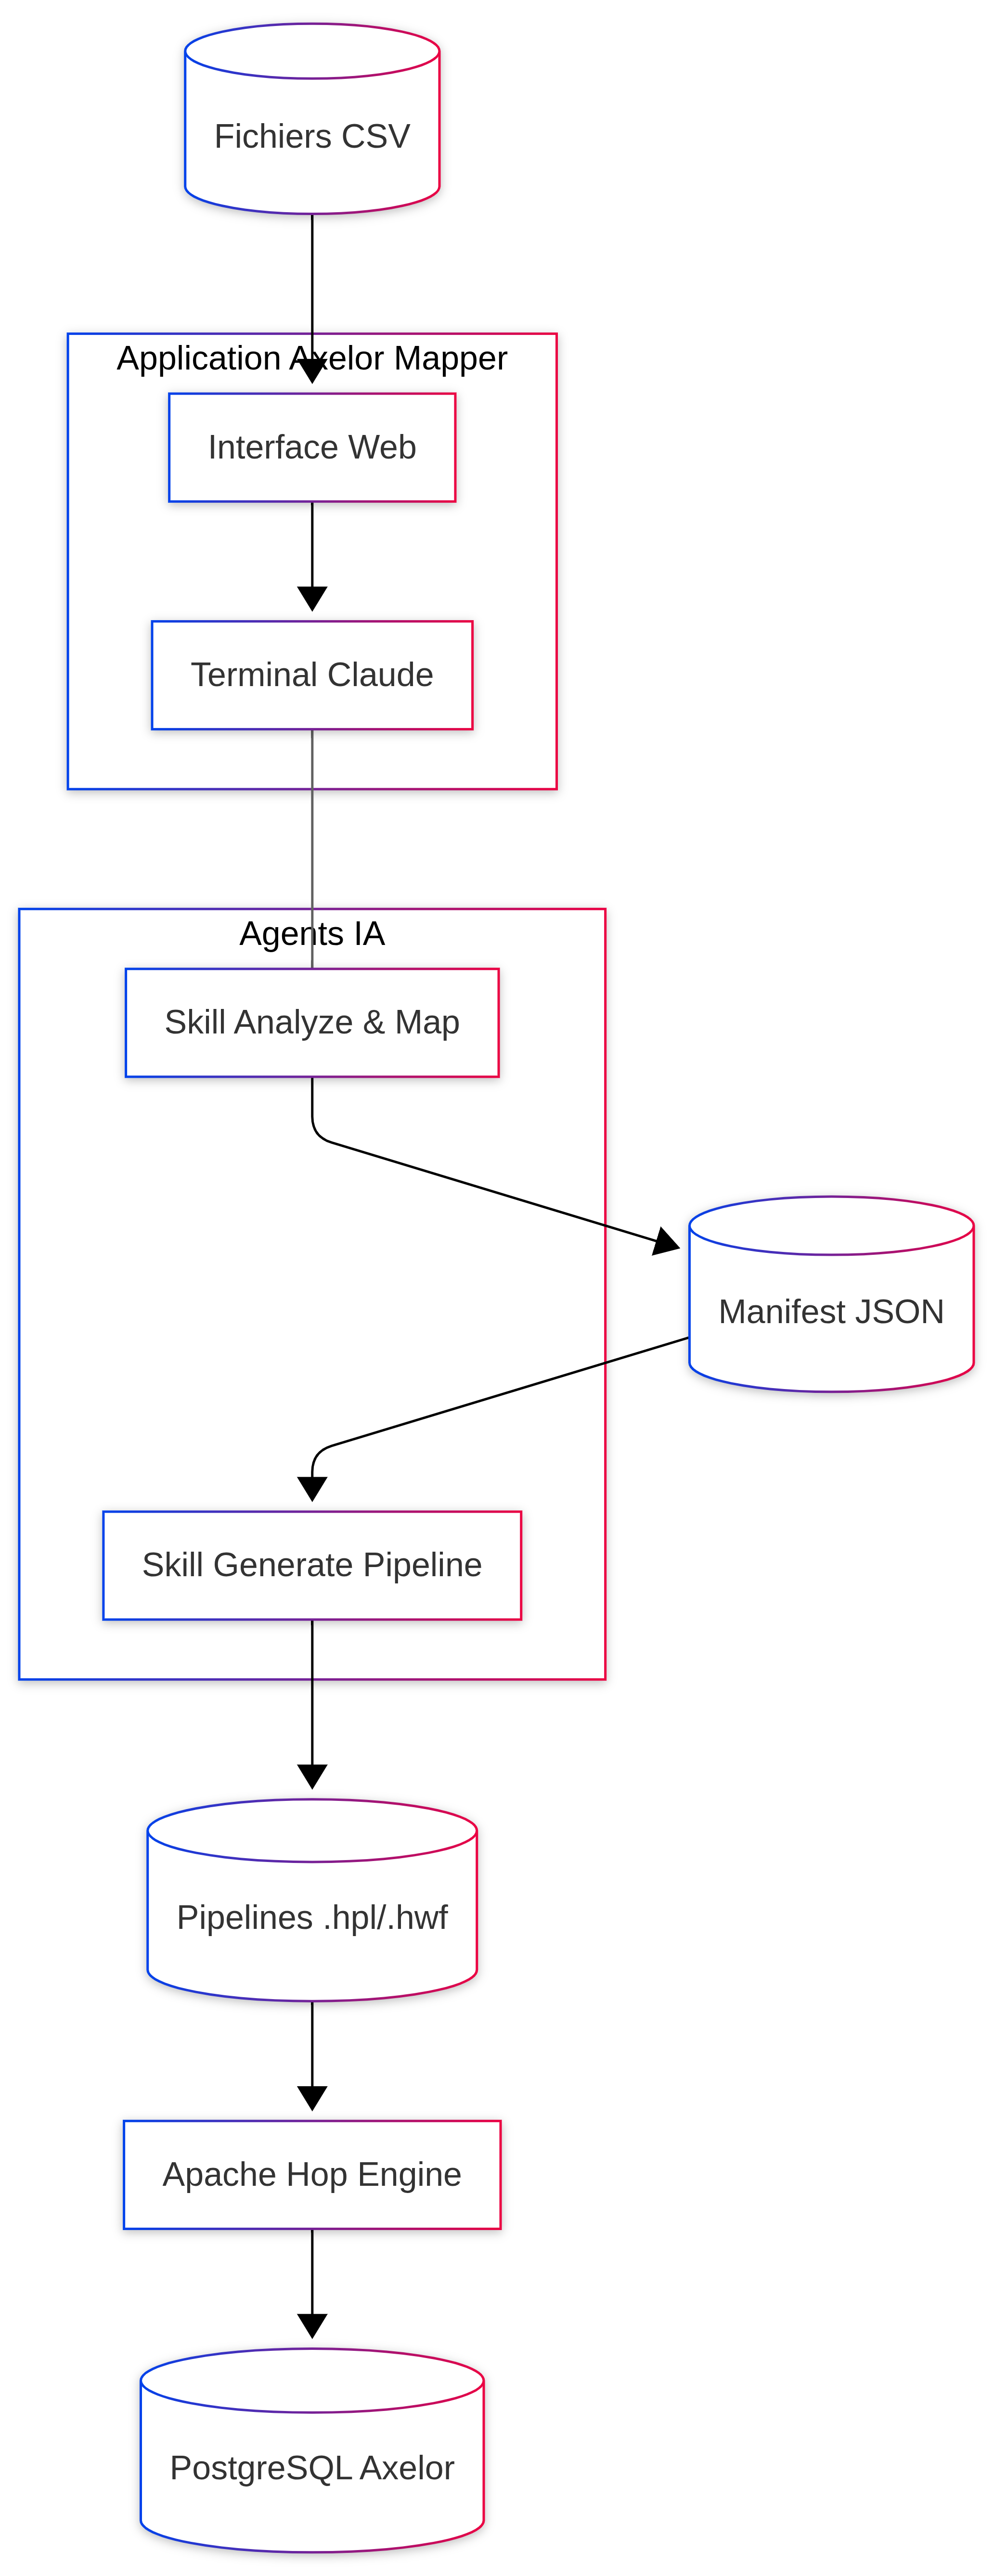
\includegraphics[width=0.6\textwidth]{Architecture-generale.png}
    \caption{Architecture globale du framework AOS-ETL}
    \label{fig:archi-generale}
\end{figure}

%% ============================================================
\section{Sécurité et conformité RGPD}
\label{sec:securite}
%% ============================================================

\subsection{Mesures de sécurité actuelles}

\begin{itemize}
    \item \textbf{Accès direct PostgreSQL~:} les credentials de la base cible sont saisis dans l'interface au démarrage de la session et restent côté serveur backend. Aucun appel API vers l'application Axelor n'est effectué.
    \item \textbf{Sessions éphémères~:} chaque session est identifiée par un UUID aléatoire. Il n'y a pas de système d'authentification utilisateur — l'outil est conçu pour un usage interne en environnement contrôlé.
    \item \textbf{Clés API~:} l'accès à Claude nécessite une authentification standard via le CLI (\texttt{claude login}). Aucune clé n'est stockée par l'application.
\end{itemize}

\subsection{Conformité RGPD et données personnelles}

L'agent IA (Claude) traite les fichiers CSV fournis par l'utilisateur dans son contexte de conversation. Si ces fichiers contiennent des données personnelles (noms, adresses, emails de clients réels), ces données sont transmises au modèle hébergé par Anthropic.

\textbf{Limitation actuelle~:} l'outil ne supporte pas l'anonymisation automatique des données avant leur envoi au modèle. Il est donc de la \textbf{responsabilité de l'utilisateur} de~:
\begin{itemize}
    \item Utiliser des fichiers d'entrée anonymisés ou fictifs lors de la phase de mapping ;
    \item Travailler sur une base de données de test (et non de production) ;
    \item Ne pas exposer de données personnelles réelles à l'agent IA.
\end{itemize}

Cette approche est conforme à l'usage en environnement de développement, où les données de test sont généralement synthétiques. L'anonymisation automatique des données en amont constitue une perspective d'amélioration future.

%% ============================================================
\section*{Conclusion}
%% ============================================================

Ce chapitre a présenté les choix technologiques justifiés par benchmark, l'architecture à deux flux découplés par le manifeste JSON, et les mesures de sécurité. Le chapitre suivant aborde l'implémentation concrète de chaque composant.

\chapter{Implémentation}
\label{chap:implementation}

Ce chapitre décrit comment la solution est construite~: l'environnement de développement, puis les réalisations concrètes (pipelines ETL, skills IA, application Mapper) avec captures d'écran commentées.

%% ============================================================
\section{Environnement et outils de développement}
%% ============================================================

\begin{table}[H]
  \centering
  \renewcommand{\arraystretch}{1.4}
  \begin{tabular}{p{4cm} p{4cm} p{5.5cm}}
    \toprule
    \rowcolor{gray!20}
    \textbf{Catégorie} & \textbf{Outil} & \textbf{Usage} \\
    \midrule
    \rowcolor{gray!5}
    IDE             & VS Code               & Développement Python/React/skills \\
    ETL             & Apache Hop 2.0        & Conception et exécution des pipelines \\
    \rowcolor{gray!5}
    Base de données & PostgreSQL 15         & Base cible Axelor Open Suite \\
    Versionnement   & Git                   & Pipelines XML, manifestes, code \\
    \rowcolor{gray!5}
    Agent IA        & Claude CLI            & Exécution des skills \\
    Backend         & Python 3.10 + FastAPI & API REST + WebSocket \\
    \rowcolor{gray!5}
    Frontend        & React 18 + TypeScript & Interface utilisateur + xterm.js \\
    Gestion projet  & Redmine               & Suivi des tickets \\
    \bottomrule
  \end{tabular}
  \caption{Environnement et outils de développement}
  \label{tab:outils-dev}
\end{table}

%% ============================================================
\section{Présentation des réalisations}
%% ============================================================

\subsection{Pipelines d'import (Apache Hop)}

\subsubsection{Structure du projet}

Le projet est organisé selon la structure suivante, versionnée sous Git~:

\begin{figure}[H]
    \centering
    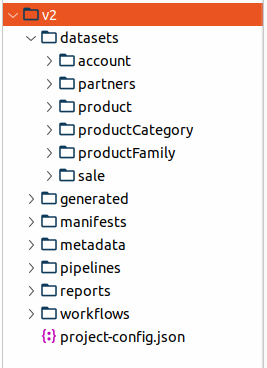
\includegraphics[width=0.6\textwidth]{structure-projet-apache-hop.png}
    \caption{Structure du projet Apache Hop}
    \label{fig:structure-projet}
\end{figure}

Les dossiers principaux sont~:
\begin{itemize}
    \item \texttt{datasets/} — fichiers CSV source organisés par entité ;
    \item \texttt{pipelines/} — fichiers \texttt{.hpl} (pipelines de transformation) ;
    \item \texttt{workflows/} — fichiers \texttt{.hwf} (orchestrateurs) ;
    \item \texttt{manifests/} — fichiers JSON décrivant le mapping ;
    \item \texttt{metadata/rdbms/} — configuration de la connexion PostgreSQL ;
    \item \texttt{reports/} — rapports d'erreurs générés à l'exécution.
\end{itemize}

\subsubsection{Entité Produits}

Le module comprend quatre pipelines orchestrés par le workflow \texttt{import\_product}~:

\begin{figure}[H]
    \centering
    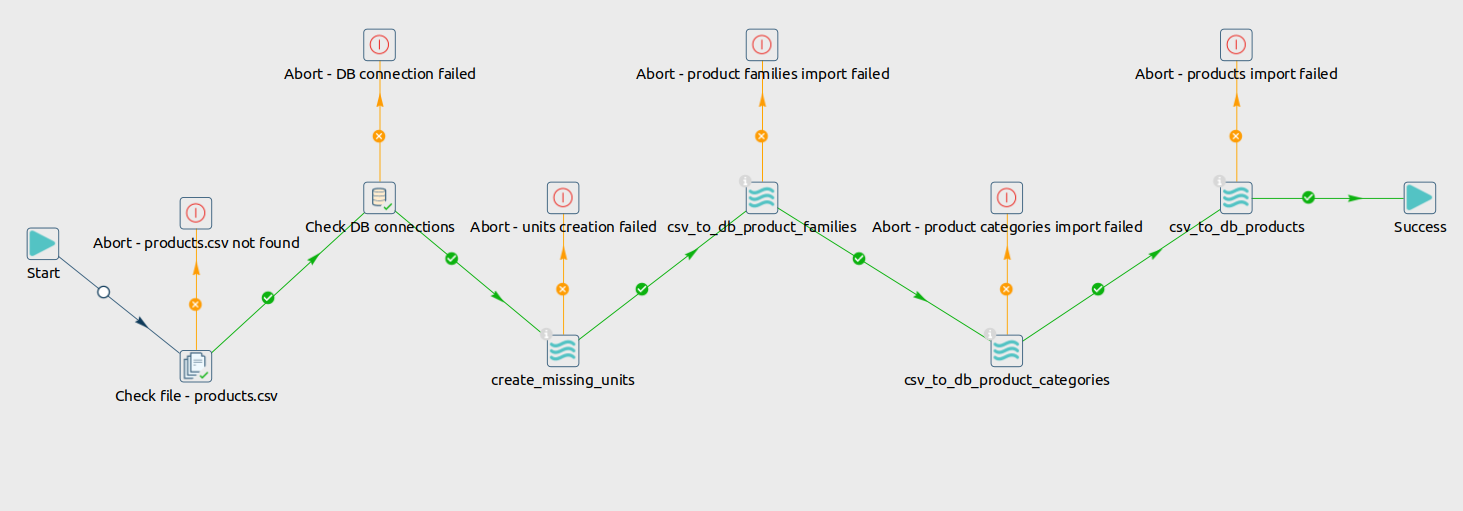
\includegraphics[width=\textwidth]{workflows-import_product.png}
    \caption{Workflow import\_product — orchestration séquentielle}
    \label{fig:workflow-product}
\end{figure}

Le workflow intègre des \textit{preflight checks}~: vérification de l'existence du fichier CSV et test de la connexion BD. En cas d'échec, l'exécution est interrompue par une action Abort.

\paragraph{Pipeline de création des unités manquantes} Ce pipeline implémente le pattern \textit{find-or-create}~: il lit le CSV principal des produits, extrait les noms d'unités référencées, déduplique, vérifie lesquelles existent déjà en base, et insère uniquement les manquantes.

\begin{figure}[H]
    \centering
    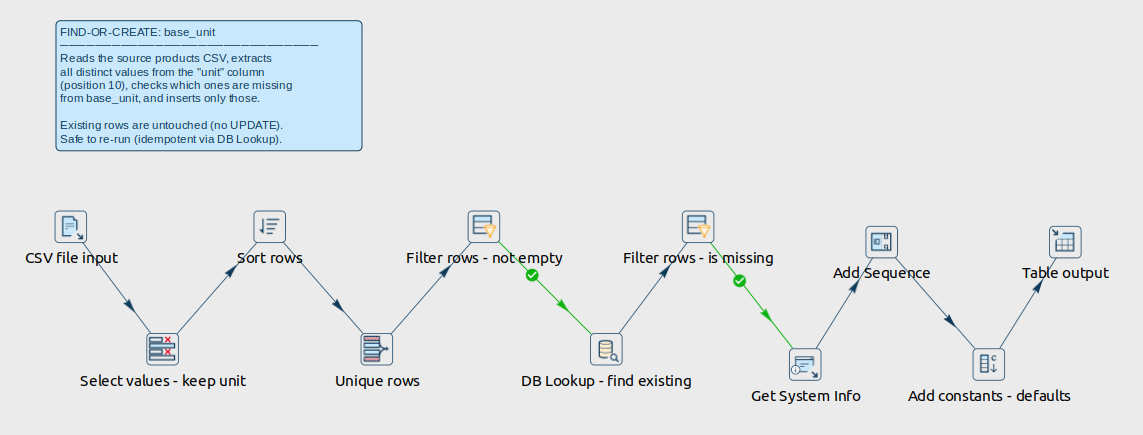
\includegraphics[width=\textwidth]{create-missing-units.png}
    \caption{Pipeline create\_missing\_units — création des unités manquantes}
    \label{fig:create-missing-units}
\end{figure}

\paragraph{Pipeline d'import des familles} Import des familles de produits avec le pattern upsert simple (import\_id + name, pas de FK à résoudre).

\begin{figure}[H]
    \centering
    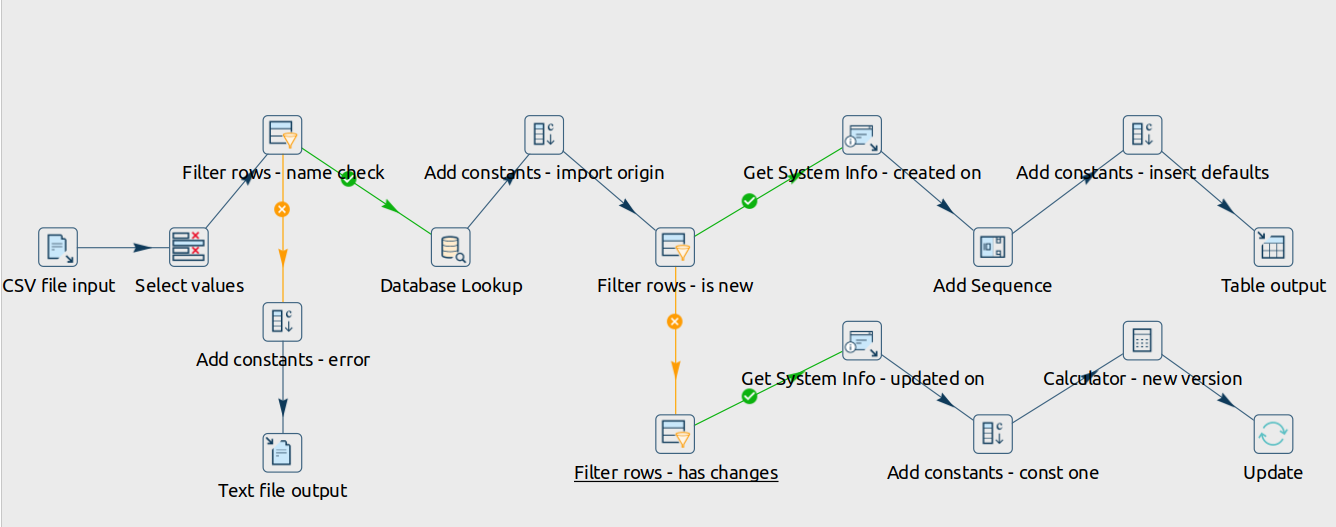
\includegraphics[width=\textwidth]{csv_to_db_product_families.png}
    \caption{Pipeline csv\_to\_db\_product\_families}
    \label{fig:pipeline-families}
\end{figure}

\paragraph{Pipeline d'import des catégories} Import des catégories de produits, même pattern que les familles.

\begin{figure}[H]
    \centering
    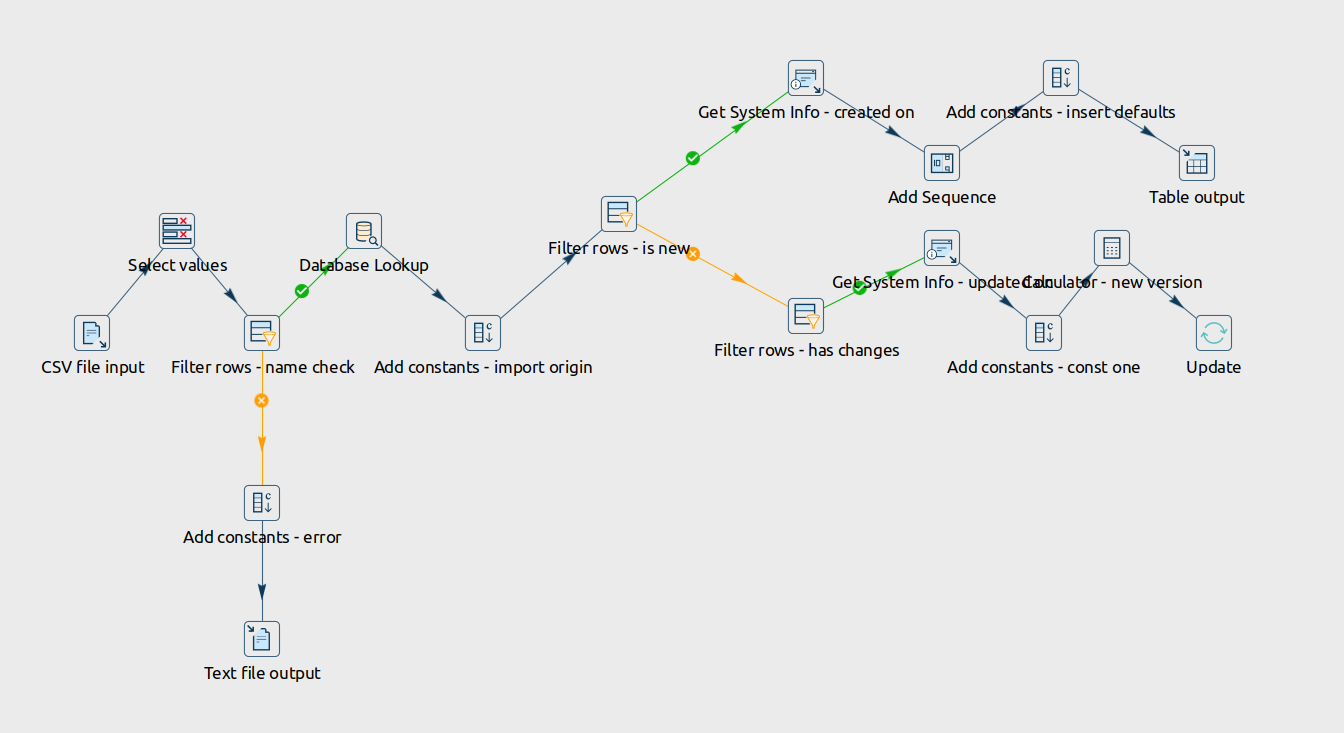
\includegraphics[width=\textwidth]{csv_to_db_product_categories.png}
    \caption{Pipeline csv\_to\_db\_product\_categories}
    \label{fig:pipeline-categories}
\end{figure}

\paragraph{Pipeline d'import des produits} Le pipeline le plus complexe de l'entité~: import des produits avec résolution de multiples FK (unité, famille, catégorie, devise, fournisseur), gestion des champs calculés (full\_name), et écriture dans des tables secondaires (account\_management).

\begin{figure}[H]
    \centering
    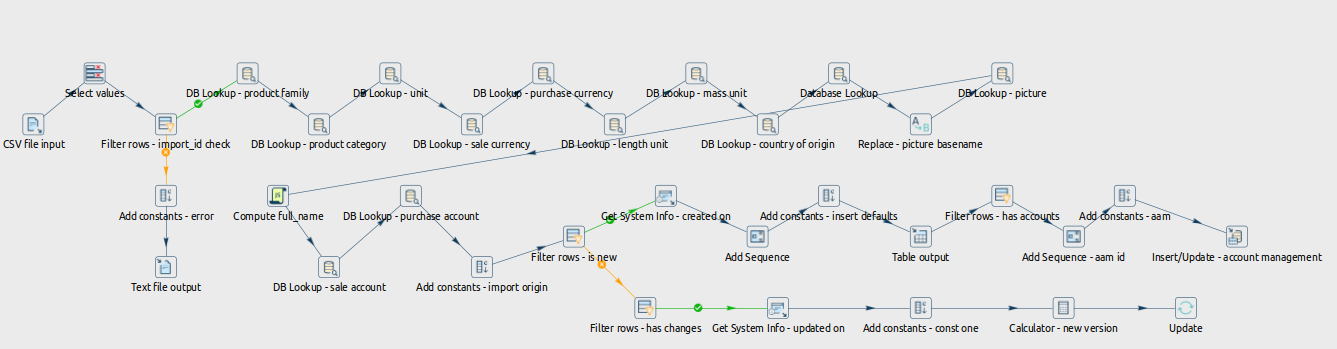
\includegraphics[width=\textwidth]{csv_to_db_products.png}
    \caption{Pipeline csv\_to\_db\_products — import complet des produits}
    \label{fig:pipeline-products}
\end{figure}

\subsubsection{Entité Partenaires}

Six pipelines orchestrés par le workflow \texttt{import\_partners}~:

\begin{figure}[H]
    \centering
    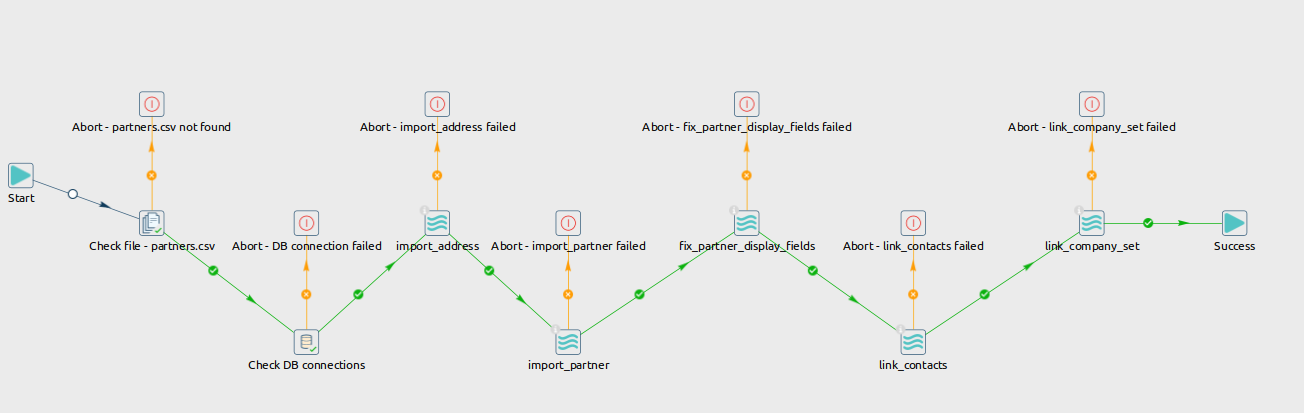
\includegraphics[width=\textwidth]{import_partners.png}
    \caption{Workflow import\_partners — orchestration de l'entité partenaires}
    \label{fig:workflow-partners}
\end{figure}

L'ordre est imposé par les dépendances~: adresses avant partenaires, liaisons après les deux.

\paragraph{Pipeline d'import des adresses} Ce pipeline lit le fichier \texttt{partners.csv} et en extrait les adresses embarquées (format texte libre~: ``70 RUE PASTORELLI | 06000 NICE | FRANCE''). Il parse chaque adresse en composantes (rue, code postal + ville, pays), déduplique les adresses identiques, et insère uniquement celles qui n'existent pas encore en base. Le mode est \textit{insert-only}~: pas d'update, car une adresse ne change pas.

\begin{figure}[H]
    \centering
    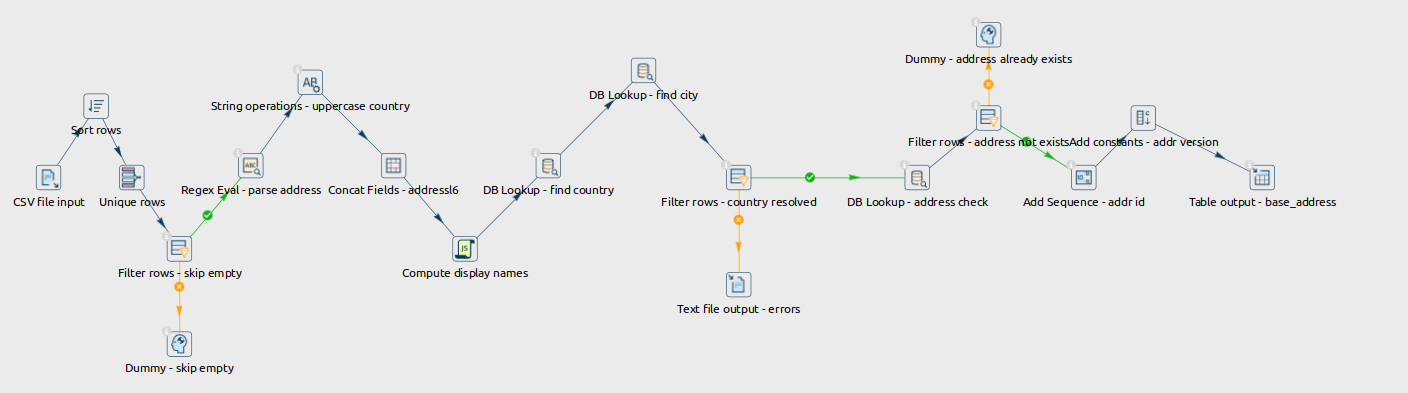
\includegraphics[width=\textwidth]{import_address.png}
    \caption{Pipeline import\_address — parsing et insertion des adresses}
    \label{fig:pipeline-address}
\end{figure}

\paragraph{Pipeline d'import des partenaires} Ce pipeline implémente le pattern upsert complet pour les partenaires. Il résout les FK vers~: l'adresse principale (par import\_id), la devise (par code), le mode de paiement, les conditions de paiement, la catégorie partenaire et la position fiscale. Les partenaires sont classés en deux types~: entreprises (partnerTypeSelect=1) et contacts (partnerTypeSelect=2).

\begin{figure}[H]
    \centering
    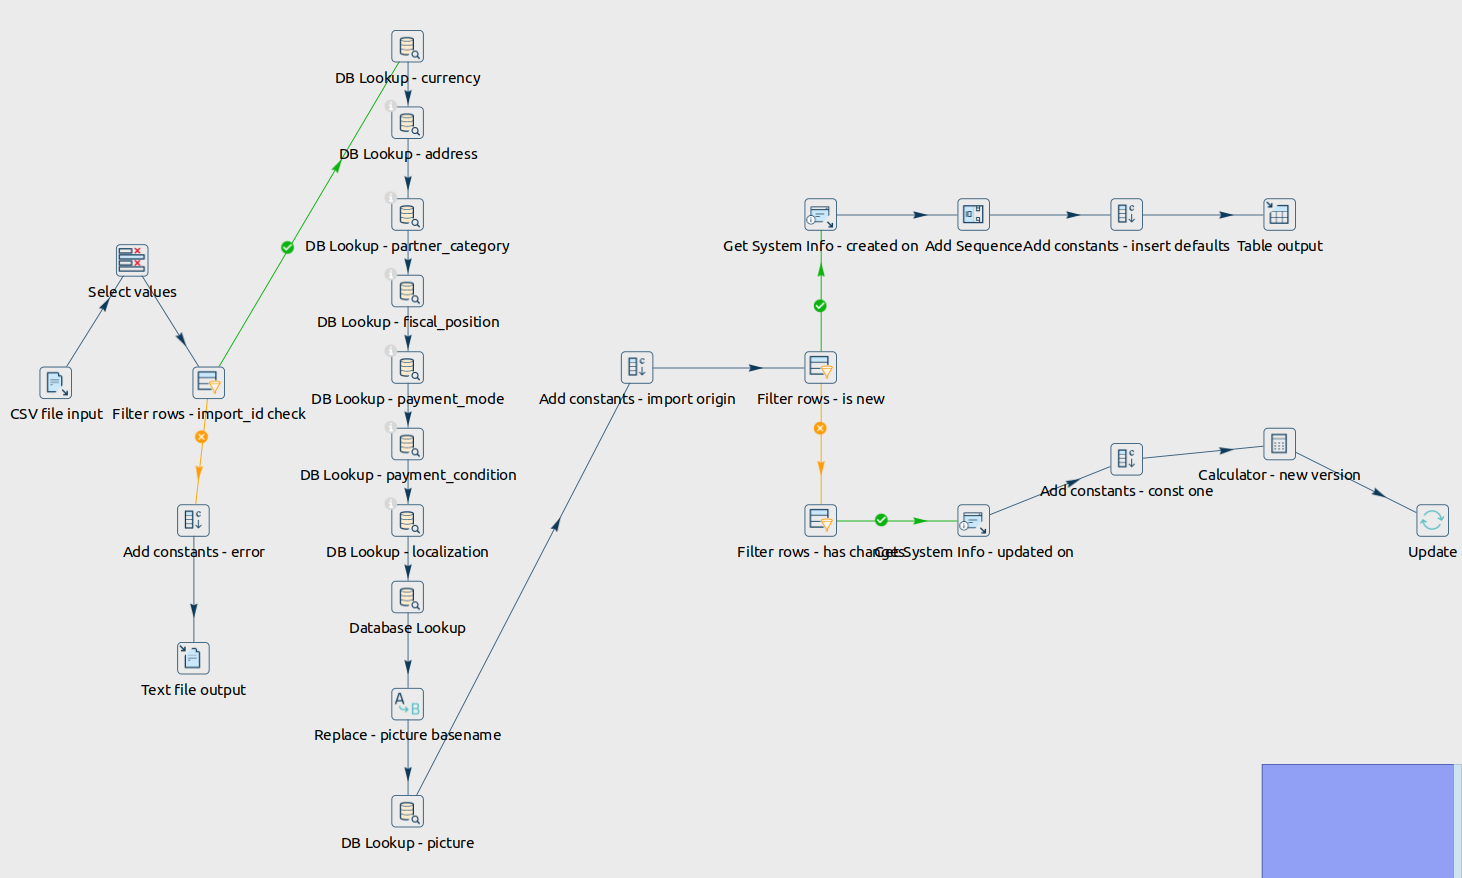
\includegraphics[width=\textwidth]{import_partner.png}
    \caption{Pipeline import\_partner — import avec résolution FK multiples}
    \label{fig:pipeline-partner}
\end{figure}

\paragraph{Pipeline de calcul des champs d'affichage} Ce pipeline est de type \textit{post-SQL}~: il ne lit pas de CSV mais exécute des requêtes SQL directement sur la base pour calculer des champs dérivés. Il génère les séquences partenaires (\texttt{partner\_seq}), construit les champs d'affichage (\texttt{full\_name}, \texttt{simple\_full\_name}), et crée les enregistrements dans la table \texttt{base\_partner\_address} qui lie chaque partenaire à son adresse de facturation.

\begin{figure}[H]
    \centering
    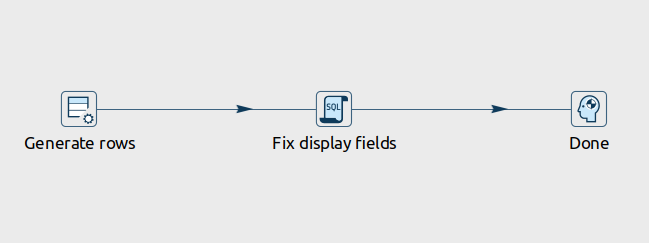
\includegraphics[width=\textwidth]{fix_partner_display_fields.png}
    \caption{Pipeline fix\_partner\_display\_fields — calcul des champs dérivés par SQL}
    \label{fig:pipeline-fix-display}
\end{figure}

\paragraph{Pipeline de liaison partenaire-adresse} Ce pipeline peuple la table de jonction \texttt{base\_partner\_address} qui associe chaque partenaire à ses adresses (facturation, livraison). Il lit un CSV dédié contenant les paires (partner\_importId, address\_importId), résout les deux FK, vérifie que la liaison n'existe pas déjà (idempotence), puis insère.

\begin{figure}[H]
    \centering
    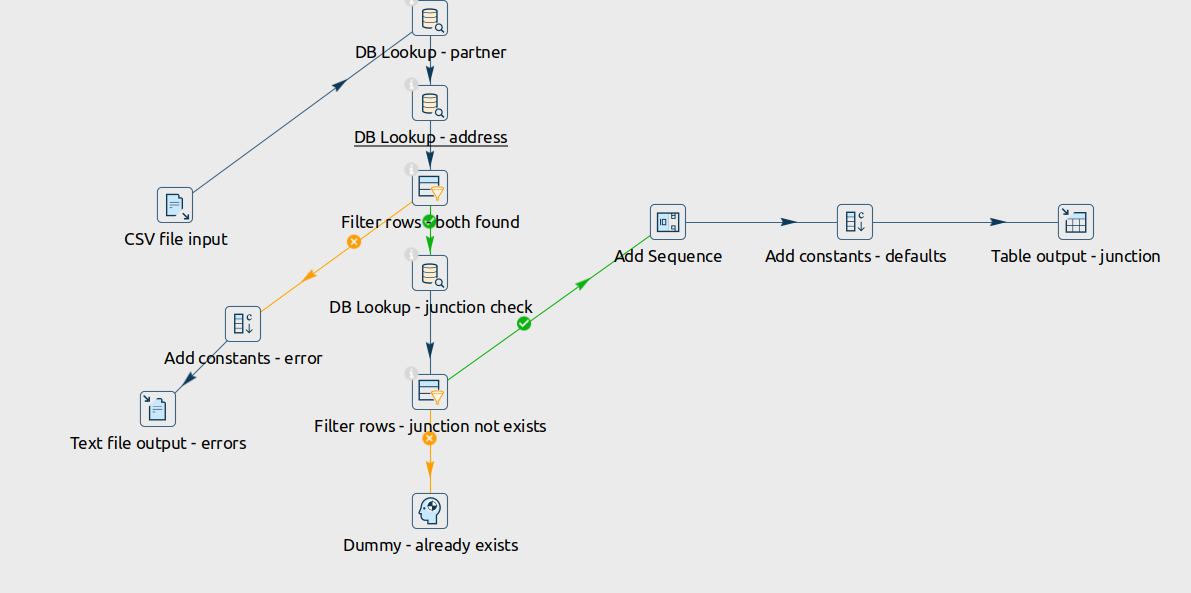
\includegraphics[width=\textwidth]{link_partner_address.png}
    \caption{Pipeline link\_partner\_address — liaison partenaire-adresse}
    \label{fig:pipeline-link-address}
\end{figure}

\paragraph{Pipeline de liaison partenaire-société} Ce pipeline associe les partenaires à leurs sociétés dans la table de jonction Many-to-Many. Il résout le partenaire par import\_id et la société par code, vérifie l'absence de doublon, puis insère la liaison.

\begin{figure}[H]
    \centering
    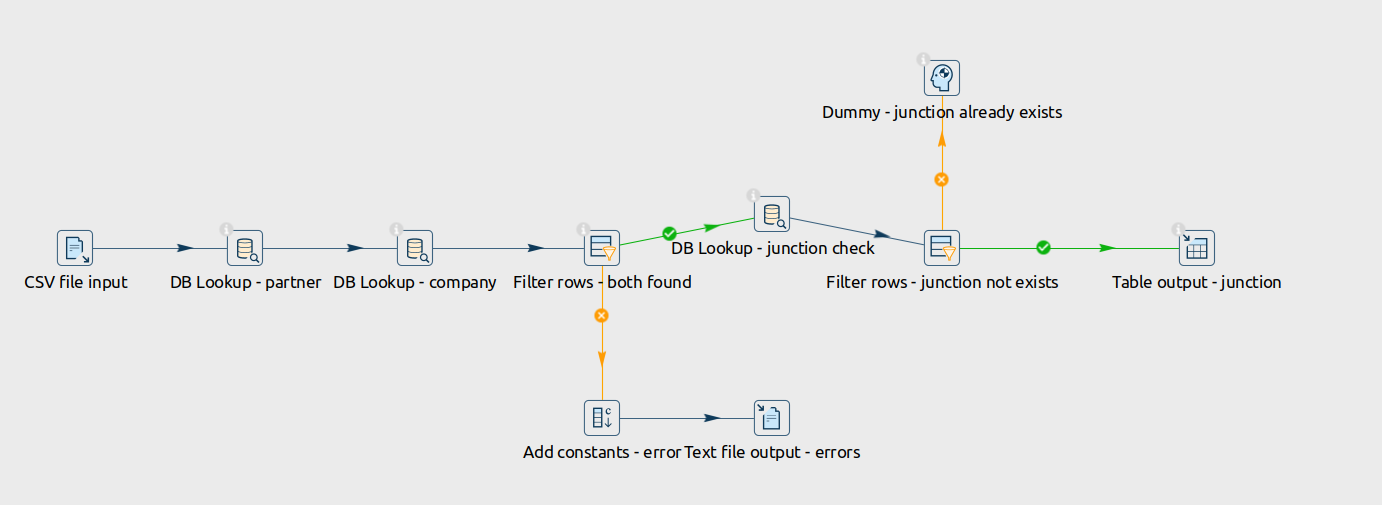
\includegraphics[width=\textwidth]{link_company_set.png}
    \caption{Pipeline link\_company\_set — liaison partenaire-société}
    \label{fig:pipeline-link-company}
\end{figure}

\subsubsection{Entité Commandes de vente}

Quatre pipelines orchestrés par le workflow \texttt{import\_sale\_orders\_v3}~:

\begin{figure}[H]
    \centering
    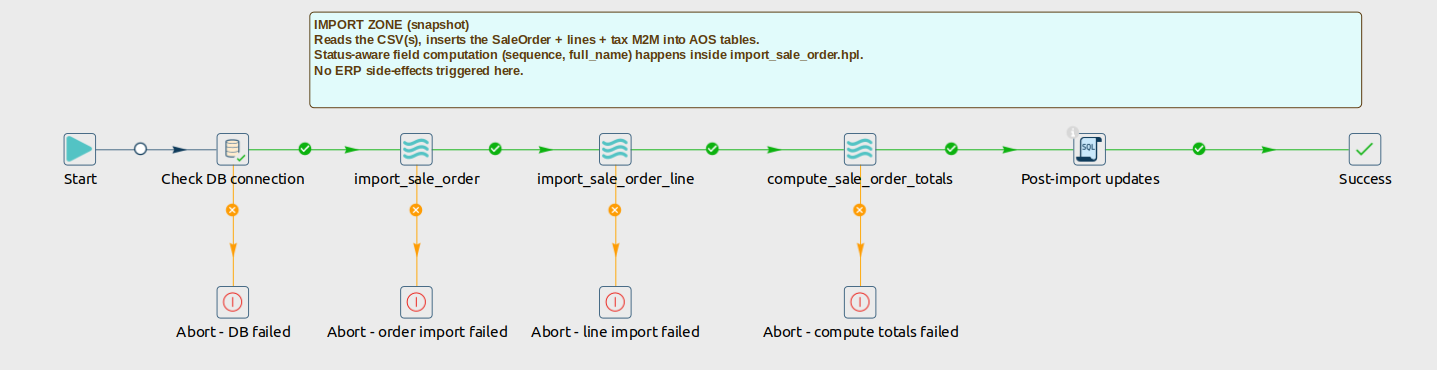
\includegraphics[width=\textwidth]{import_sale_orders_v3.png}
    \caption{Workflow import\_sale\_orders}
    \label{fig:workflow-sale}
\end{figure}

\paragraph{Pipeline d'import des commandes} Ce pipeline implémente le pattern upsert avec des particularités~: il résout 12 FK (client, contact, adresses, commercial, équipe, mode de paiement, condition de paiement, devise, société, paramètres d'impression, confirmé par). Il intègre un \textit{status\_sequence} — un branchement conditionnel qui génère le numéro de commande différemment selon le statut (brouillon vs confirmé). Un champ calculé \texttt{full\_name} est produit à partir du numéro de séquence et du nom du client.

\begin{figure}[H]
    \centering
    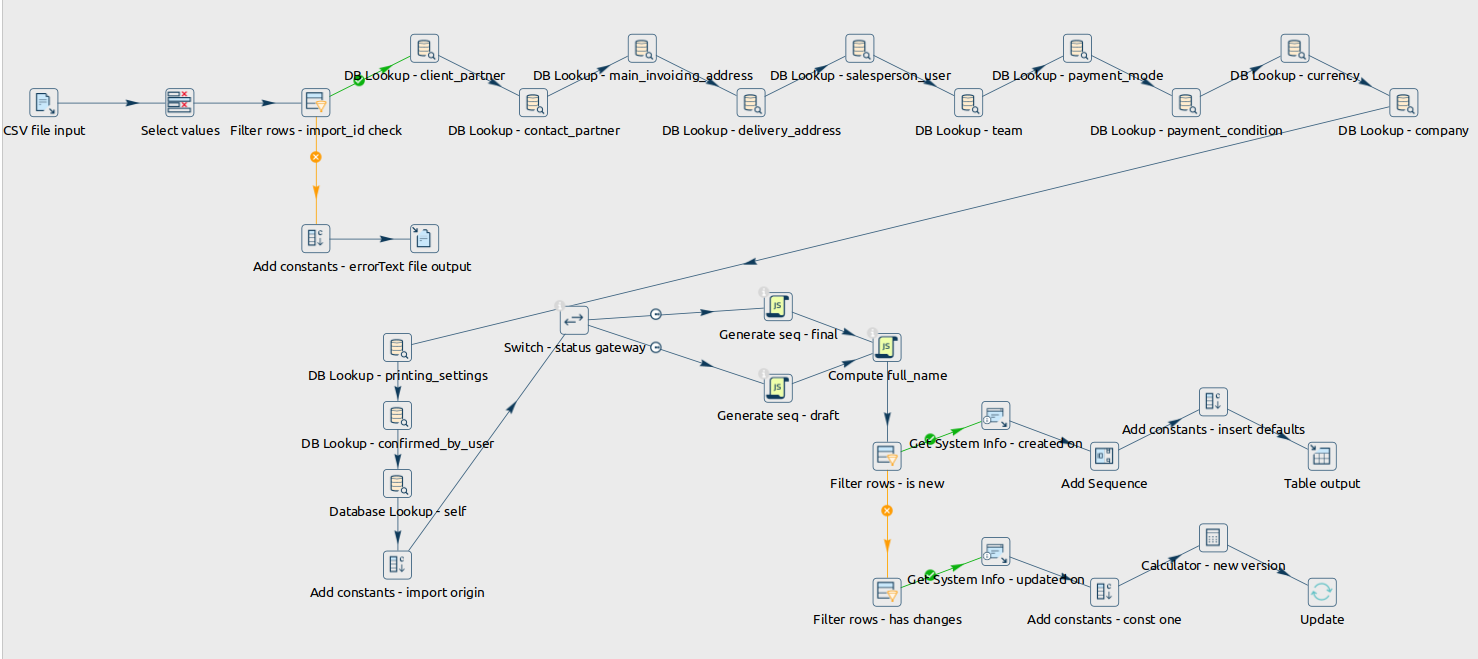
\includegraphics[width=\textwidth]{import_sale_order.png}
    \caption{Pipeline import\_sale\_order — import avec status\_sequence et 12 FK}
    \label{fig:pipeline-sale-order}
\end{figure}

\paragraph{Pipeline d'import des lignes de commande} Ce pipeline importe les lignes de commande. Il résout les FK vers la commande parente, le produit et l'unité. Un champ calculé \texttt{price\_discounted} applique la remise selon le type (pourcentage ou montant fixe) et recalcule les totaux HT et TTC. Après insertion, une jonction inline associe chaque ligne à sa taxe dans la table M2M.

\begin{figure}[H]
    \centering
    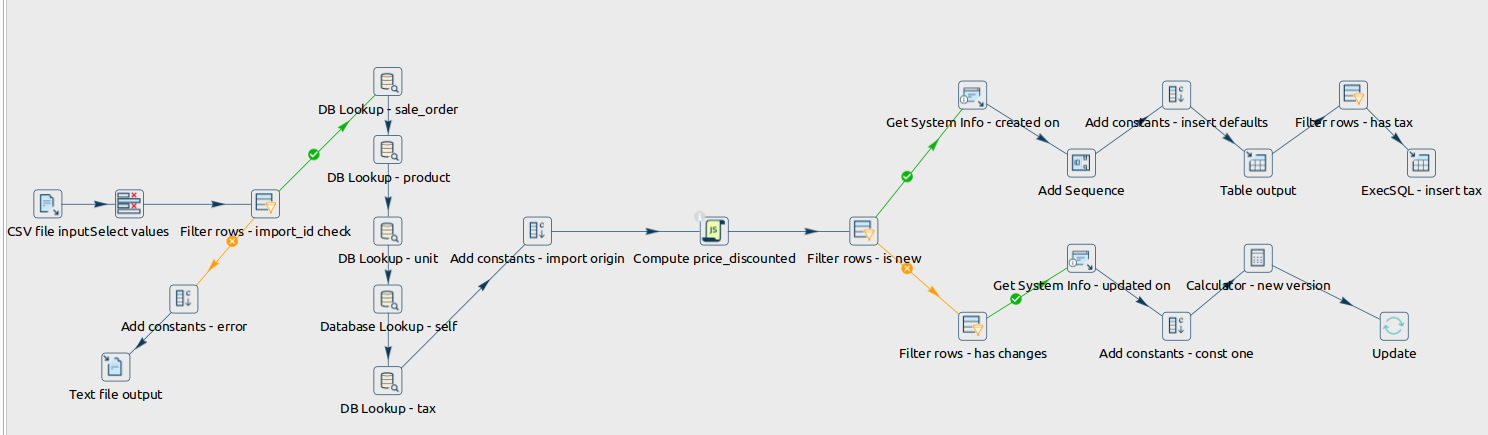
\includegraphics[width=\textwidth]{import_sale_order_line.png}
    \caption{Pipeline import\_sale\_order\_line — lignes avec calcul de remise}
    \label{fig:pipeline-sale-line}
\end{figure}

\paragraph{Pipeline de jonction lignes-taxes} Ce pipeline peuple la table de jonction entre les lignes de commande et les taxes applicables. Il lit un CSV dédié, résout la ligne de commande par import\_id, vérifie que le lookup a réussi, puis insère directement dans la table de jonction.

\begin{figure}[H]
    \centering
    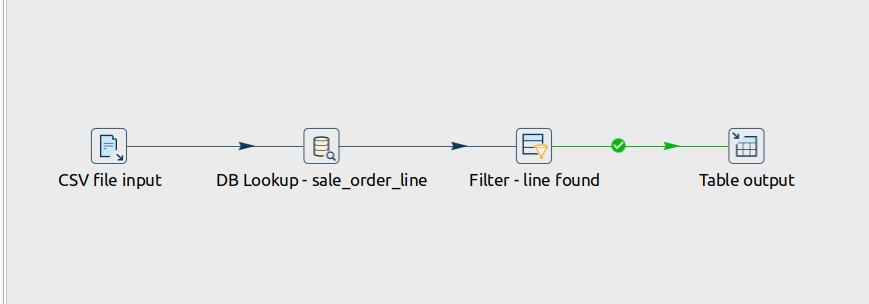
\includegraphics[width=\textwidth]{import_sale_order_line_tax_set.png}
    \caption{Pipeline import\_sale\_order\_line\_tax\_set — jonction lignes-taxes}
    \label{fig:pipeline-sale-tax}
\end{figure}

\paragraph{Pipeline de calcul des totaux} Ce pipeline post-traitement calcule les totaux des commandes à partir des lignes. Il lit les lignes avec leurs taxes via une requête SQL, calcule les montants de taxe par groupe (commande + taux), insère un résumé dans la table des taxes, puis agrège les totaux (HT, TVA, TTC) et met à jour l'en-tête de commande.

\begin{figure}[H]
    \centering
    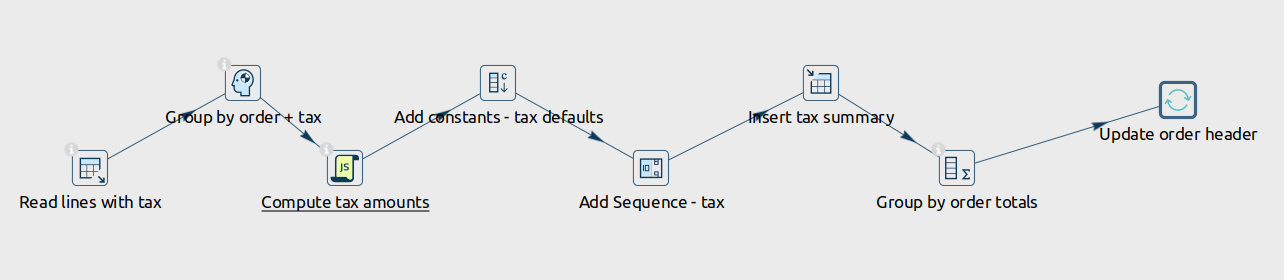
\includegraphics[width=\textwidth]{compute_sale_order_totals.png}
    \caption{Pipeline compute\_sale\_order\_totals — calcul et mise à jour des totaux}
    \label{fig:pipeline-sale-totals}
\end{figure}

\subsubsection{Entité Factures}

Six pipelines orchestrés par le workflow \texttt{import\_invoices}. C'est l'entité de validation~: une facture ventilable prouve l'intégrité de toute la chaîne d'import.

\begin{figure}[H]
    \centering
    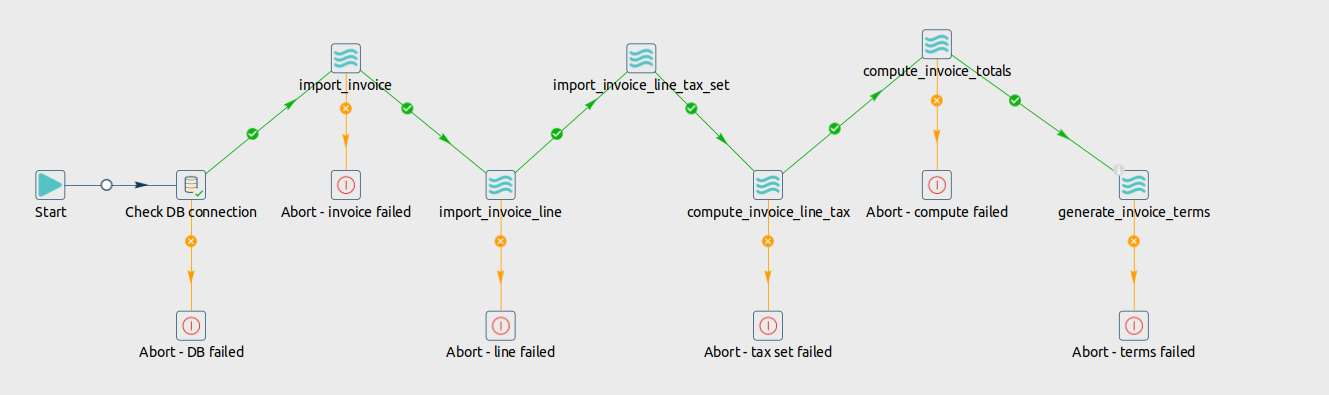
\includegraphics[width=\textwidth]{import_invoices.png}
    \caption{Workflow import\_invoices}
    \label{fig:workflow-invoices}
\end{figure}

\paragraph{Pipeline d'import des factures} — Insert-only avec 8 FK, blocking check (DBJoin), partner\_account conditionnel, journal par défaut, et champs calculés (\texttt{invoice\_id}, validation fields).

\begin{figure}[H]
    \centering
    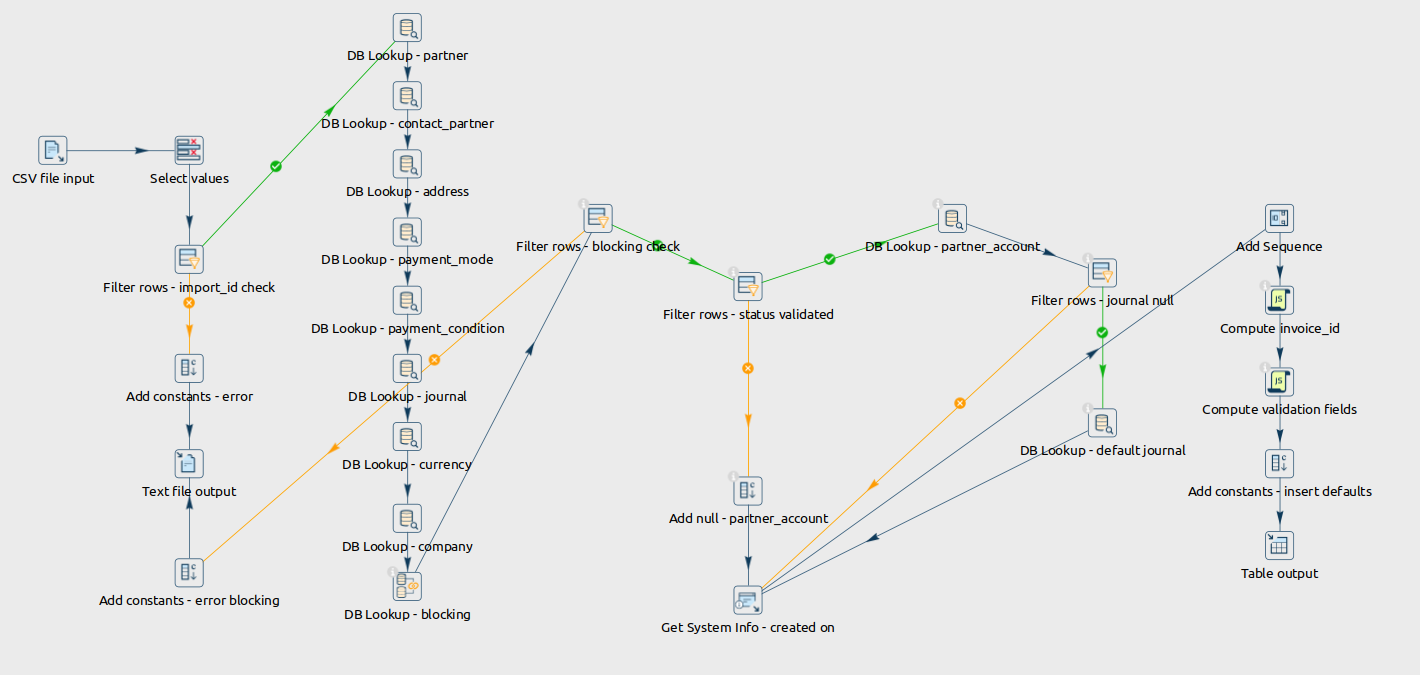
\includegraphics[width=\textwidth]{import_invoice.png}
    \caption{Pipeline import\_invoice}
    \label{fig:pipeline-invoice}
\end{figure}

\paragraph{Pipeline d'import des lignes de facture} — Insert-only avec FK vers facture (+ extra\_returns société), produit, compte comptable (dual-key), unité. Script de calcul des totaux.

\begin{figure}[H]
    \centering
    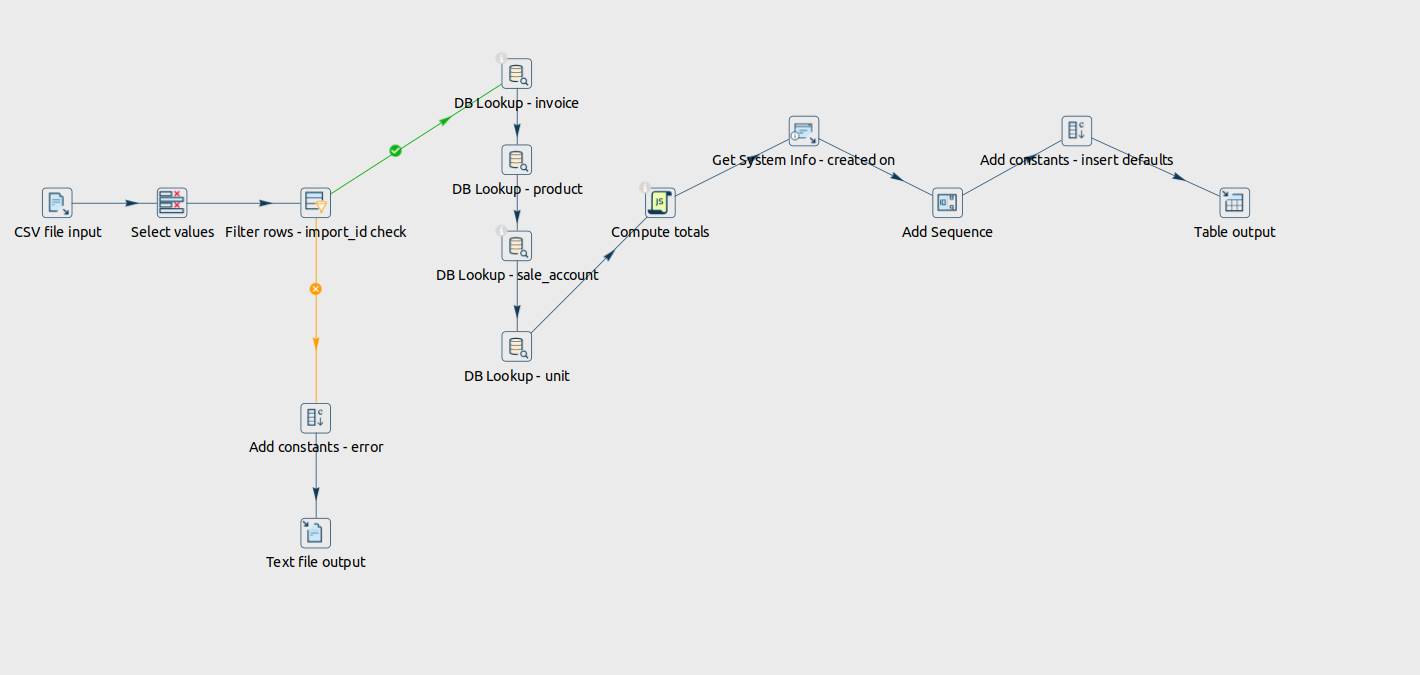
\includegraphics[width=\textwidth]{import_invoice_line.png}
    \caption{Pipeline import\_invoice\_line}
    \label{fig:pipeline-invoice-line}
\end{figure}

\paragraph{Pipeline de jonction lignes-taxes (factures)} — Jonction M2M lignes-taxes.

\begin{figure}[H]
    \centering
    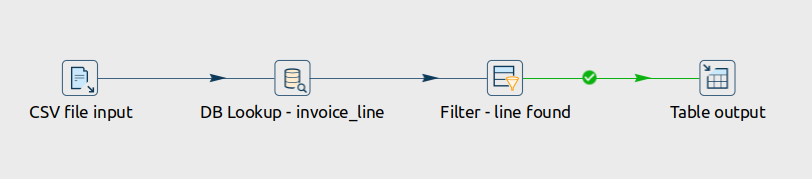
\includegraphics[width=\textwidth]{import_invoice_line_tax_set.png}
    \caption{Pipeline import\_invoice\_line\_tax\_set}
    \label{fig:pipeline-invoice-tax-set}
\end{figure}

\paragraph{Pipeline de calcul des taxes par ligne} — Post-SQL reproduisant \texttt{TaxInvoiceLine.creates()}~: calcul taxe par ligne, détermination du compte d'imputation.

\begin{figure}[H]
    \centering
    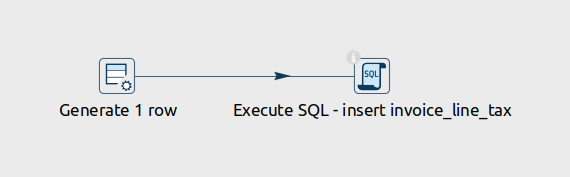
\includegraphics[width=\textwidth]{compute_invoice_line_tax.png}
    \caption{Pipeline compute\_invoice\_line\_tax}
    \label{fig:pipeline-invoice-line-tax}
\end{figure}

\paragraph{Pipeline de calcul des totaux (factures)} — Agrégation HT/TVA/TTC et mise à jour de l'en-tête + montants restants.

\begin{figure}[H]
    \centering
    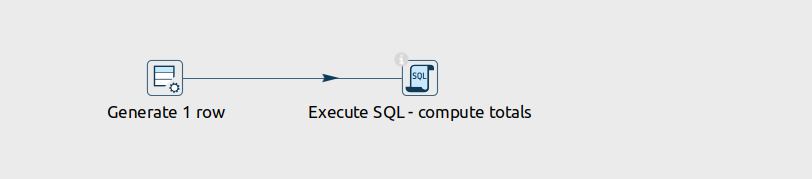
\includegraphics[width=\textwidth]{compute_invoice_totals.png}
    \caption{Pipeline compute\_invoice\_totals}
    \label{fig:pipeline-invoice-totals}
\end{figure}

\paragraph{Pipeline de génération des échéances} — Génération des échéances à partir des conditions de paiement (date + pourcentage du TTC).

\begin{figure}[H]
    \centering
    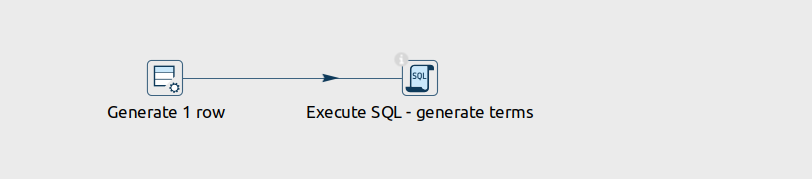
\includegraphics[width=\textwidth]{generate_invoice_terms.png}
    \caption{Pipeline generate\_invoice\_terms}
    \label{fig:pipeline-invoice-terms}
\end{figure}

\subsubsection{Rapports d'erreurs}

Chaque pipeline génère automatiquement un rapport d'erreurs au format CSV dans le dossier \texttt{reports/}. Lorsqu'un enregistrement ne peut pas être importé (FK non résolue, import\_id manquant, valeur invalide), il est routé vers le fichier d'erreurs correspondant au lieu d'être silencieusement ignoré.

Le rapport contient~: l'identifiant de l'enregistrement source, les champs pertinents (nom, code), et un message décrivant la cause de l'échec. Cela permet au consultant de corriger les données source et de relancer l'import — l'idempotence garantit que seuls les enregistrements corrigés seront réinsérés.

\begin{figure}[H]
    \centering
    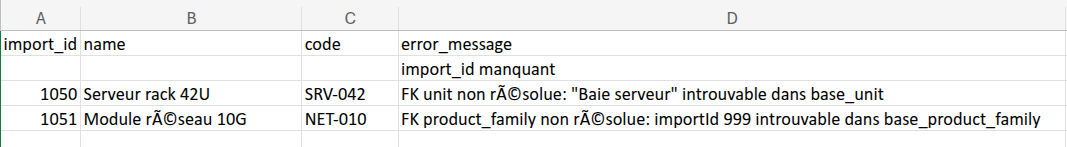
\includegraphics[width=\textwidth]{products_errors.png}
    \caption{Rapport d'erreurs produits — FK non résolues}
    \label{fig:report-products}
\end{figure}

\begin{figure}[H]
    \centering
    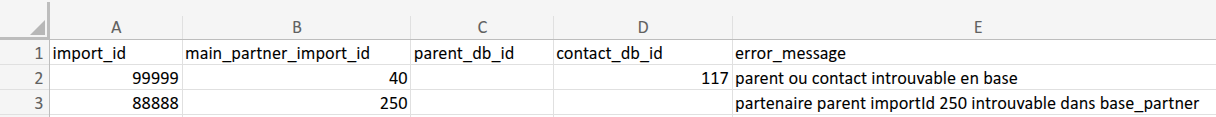
\includegraphics[width=\textwidth]{contact_link_errors.png}
    \caption{Rapport d'erreurs contacts — partenaire parent introuvable}
    \label{fig:report-contacts}
\end{figure}

%% ──────────────────────────────────────────────────────────────
\subsection{Skills IA}

Les skills IA sont des prompts structurés qui guident l'agent Claude à travers des tâches complexes. Ils sont organisés dans le dossier \texttt{.claude/commands/hop/}, chaque skill ayant son propre sous-dossier contenant un fichier principal (\texttt{.md}) et un dossier \texttt{reference/}.

\begin{figure}[H]
    \centering
    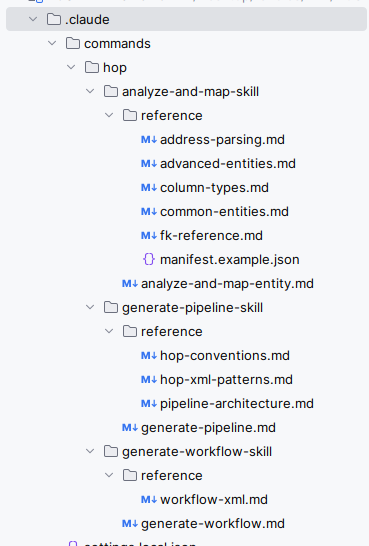
\includegraphics[width=0.6\textwidth]{skills-folder-structure.png}
    \caption{Structure des dossiers des skills IA}
    \label{fig:skills-structure}
\end{figure}

\subsubsection{Skill analyze-and-map-entity}

Ce skill (476 lignes + 6 fichiers de référence) guide l'agent à travers l'analyse d'un CSV et la production d'un manifeste JSON. Les phases sont les suivantes~:

\paragraph{Phase 0 — Connexion BD} L'agent teste immédiatement la connexion PostgreSQL avec les credentials fournis. Si la connexion réussit, toutes les vérifications FK suivantes se feront en interrogeant la base réelle. Sinon, l'agent passe en mode dégradé et se base uniquement sur les réponses de l'utilisateur.

\paragraph{Phase 1 — Lecture et classification des colonnes} L'agent lit le CSV (headers + 20 premières lignes) et requête simultanément le schéma de la table cible via \texttt{information\_schema} (colonnes, types, contraintes FK). Il classifie ensuite chaque colonne en croisant trois signaux~:
\begin{itemize}
    \item \textbf{Notation pointée} (confiance élevée)~: \texttt{productFamily.importId} indique directement la table cible et la stratégie de lookup ;
    \item \textbf{Pattern du nom} (confiance moyenne)~: un suffixe \texttt{Code}, \texttt{Id} ou \texttt{Name} suggère une FK ;
    \item \textbf{Échantillonnage des valeurs} (corroboration)~: faible cardinalité, valeurs courtes et homogènes signalent une FK.
\end{itemize}
Pour les cas ambigus, l'agent pose une question à l'utilisateur avec des options prédéfinies.

\paragraph{Phase 2 — Vérification en base} Pour chaque FK identifiée, l'agent exécute une requête SQL pour vérifier si les valeurs du CSV existent dans la table référencée. Il regroupe les FK par table de référence (ex~: \texttt{saleCurrency} et \texttt{purchaseCurrency} → une seule requête sur \texttt{base\_currency}). Trois résultats~: tout trouvé (preloaded), partiellement trouvé, ou rien trouvé.

\paragraph{Phase 3 — Résolution interactive} Pour chaque FK avec des valeurs manquantes, l'agent demande la stratégie à l'utilisateur~:
\begin{itemize}
    \item \textbf{Fichier séparé}~: l'utilisateur fournit un CSV dédié (l'agent applique récursivement le même processus à ce fichier) ;
    \item \textbf{Embedded (create automatically)}~: un pré-pipeline sera généré pour insérer les valeurs manquantes avant l'import principal ;
    \item \textbf{Skip}~: le champ FK restera NULL.
\end{itemize}

\paragraph{Phase 4 — Confirmation} L'agent affiche un tableau récapitulatif de toutes les résolutions FK et demande confirmation avant de passer à l'écriture.

\paragraph{Phase 5 — Écriture du manifeste} L'agent produit le fichier \texttt{manifest.json} v2.3 et l'écrit sur disque à l'emplacement choisi par l'utilisateur.

\begin{figure}[H]
    \centering
    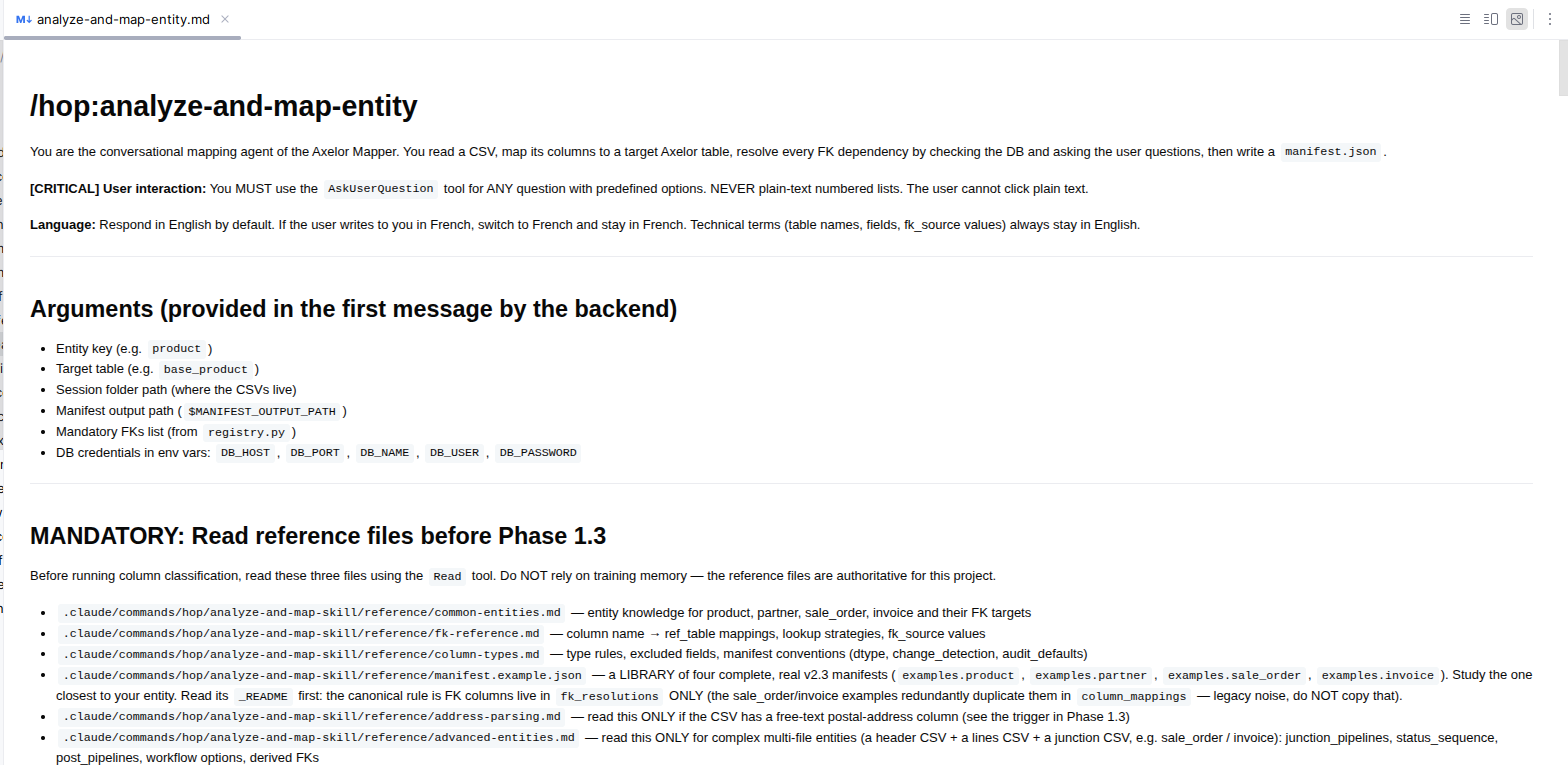
\includegraphics[width=0.7\textwidth]{analyze-and-map-skill.png}
    \caption{Extrait du skill analyze-and-map-entity}
    \label{fig:skill-analyze}
\end{figure}

\subsubsection{Le manifeste JSON — contrat entre analyse et génération}

Le manifeste est le fichier intermédiaire qui formalise le résultat de l'analyse. Il contient toutes les informations nécessaires pour que le skill de génération puisse produire les pipelines sans ambiguïté. Pour le projet, quatre manifestes ont été produits (un par module)~:

\begin{table}[H]
  \centering
  \renewcommand{\arraystretch}{1.3}
  \begin{tabular}{p{2.5cm} p{3cm} p{2cm} p{2cm} p{2cm}}
    \toprule
    \rowcolor{gray!20}
    \textbf{Manifeste} & \textbf{Import order} & \textbf{FK} & \textbf{Colonnes} & \textbf{Mode} \\
    \midrule
    \rowcolor{gray!5}
    product    & family → category → product  & 9  & 35 & upsert \\
    partner    & address → partner            & 10 & 19 & mixte \\
    \rowcolor{gray!5}
    sale\_order & order → line                 & 16 & 37 & upsert \\
    invoice    & invoice → line               & 12 & 32 & insert-only \\
    \bottomrule
  \end{tabular}
  \caption{Résumé des 4 manifestes produits}
  \label{tab:manifestes}
\end{table}

Chaque section d'entité dans le manifeste décrit~:
\begin{itemize}
    \item La table cible et le fichier source ;
    \item Le mapping colonne par colonne (source CSV → colonne DB) ;
    \item Les résolutions FK avec la stratégie de lookup et le comportement en cas d'absence ;
    \item Les champs calculés, tables secondaires, et constantes d'insertion ;
    \item L'ordre d'import respectant les dépendances entre entités.
\end{itemize}

C'est ce fichier que le skill \textit{generate-pipeline} consomme pour produire le XML Apache Hop. Sa structure est la suivante~:

\begin{verbatim}
{
  "primary_entity": "product",
  "import_order": ["product_family", "product_category", "product"],
  "pre_pipelines": [...],
  "entities": {
    "product": {
      "target_table": "base_product",
      "pipeline_name": "csv_to_db_products",
      "write_mode": "upsert",
      "source": { "file": "datasets/product/products.csv", "delimiter": ";" },
      "column_mappings": [
        { "source": "name", "target": "name", "type": "string" },
        { "source": "salePrice", "target": "sale_price", "type": "decimal" }
      ],
      "fk_resolutions": [
        {
          "source_column": "productFamily.importId",
          "target_fk_field": "product_family_id",
          "db_column": "product_family",
          "ref_table": "base_product_family",
          "strategies": ["by_import_id"],
          "fk_source": "separate_entity",
          "on_miss": "set_null"
        }
      ],
      "computed_fields": [...],
      "secondary_tables": [...],
      "change_detection_fields": ["name", "code"],
      "insert_constants": { "is_model": false }
    }
  }
}
\end{verbatim}

Chaque champ guide directement la génération du pipeline~:
\begin{itemize}
    \item \texttt{write\_mode} détermine le pattern (upsert avec UPDATE, ou insert-only sans) ;
    \item \texttt{column\_mappings} génère le bloc \texttt{Select Values} (renommage CSV → DB) et le \texttt{Table Output} ;
    \item \texttt{fk\_resolutions} génère un \texttt{DB Lookup} par FK, avec la table, la clé et le comportement en cas d'absence ;
    \item \texttt{change\_detection\_fields} génère le filtre ``has changes'' (comparaison avant/après pour l'UPDATE) ;
    \item \texttt{import\_order} détermine l'enchaînement dans le workflow.
\end{itemize}

Le manifeste supporte également des patterns avancés~:

\paragraph{Pattern embedded (création automatique de références manquantes)}
Lorsqu'une colonne CSV contient directement le nom d'une référence (ex~: \texttt{unit = "Jour ouvré"}) au lieu d'un ID, le manifeste utilise \texttt{fk\_source: "embedded"} avec un bloc \texttt{pre\_pipeline\_config}~:

\begin{verbatim}
{
  "source_column": "unit",
  "ref_table": "base_unit",
  "lookup_field": "name",
  "fk_source": "embedded",
  "pre_pipeline_config": {
    "name": "create_missing_units",
    "subdir": "product/units",
    "sequence": "base_unit_seq"
  }
}
\end{verbatim}

Cela génère un pré-pipeline qui extrait les valeurs uniques du CSV, vérifie leur existence en base, et insère les manquantes avant l'import principal.

\paragraph{Pattern parse\_config (adresses embarquées)}
Pour les entités dont une colonne contient une adresse en texte libre (``70 RUE PASTORELLI | 06000 NICE | FRANCE''), le manifeste inclut un bloc \texttt{parse\_config} qui décrit le parsing~:

\begin{verbatim}
"parse_config": {
  "type": "regex_split",
  "source_field": "address",
  "pattern": "^([^|]+)\\|\\s*(\\d+)\\s+([^|]+)\\|\\s*(.+)$",
  "groups": [
    { "name": "addr_street" },
    { "name": "addr_zip" },
    { "name": "addr_city" },
    { "name": "addr_country" }
  ],
  "pre_dedup": { "sort_field": "address", "unique_field": "address" }
}
\end{verbatim}

Cela génère un pipeline insert-only avec~: tri + déduplication, RegexEval pour splitter l'adresse, puis insertion.

\paragraph{Pattern junction\_pipelines (tables M2M)}
Les relations Many-to-Many sont décrites au niveau racine du manifeste dans \texttt{junction\_pipelines[]}~:

\begin{verbatim}
"junction_pipelines": [{
  "name": "link_partner_address",
  "source": { "file": "datasets/partners/partnerAddresses.csv" },
  "side_a": { "csv_column": "partner_importId", "ref_table": "base_partner" },
  "side_b": { "csv_column": "address_importId", "ref_table": "base_address" },
  "junction_table": "base_partner_address",
  "sequence": "base_partner_address_seq"
}]
\end{verbatim}

Cela génère un pipeline qui résout les deux côtés par lookup, vérifie l'absence de doublon (idempotence), puis insère dans la table de jonction.

\begin{figure}[H]
    \centering
    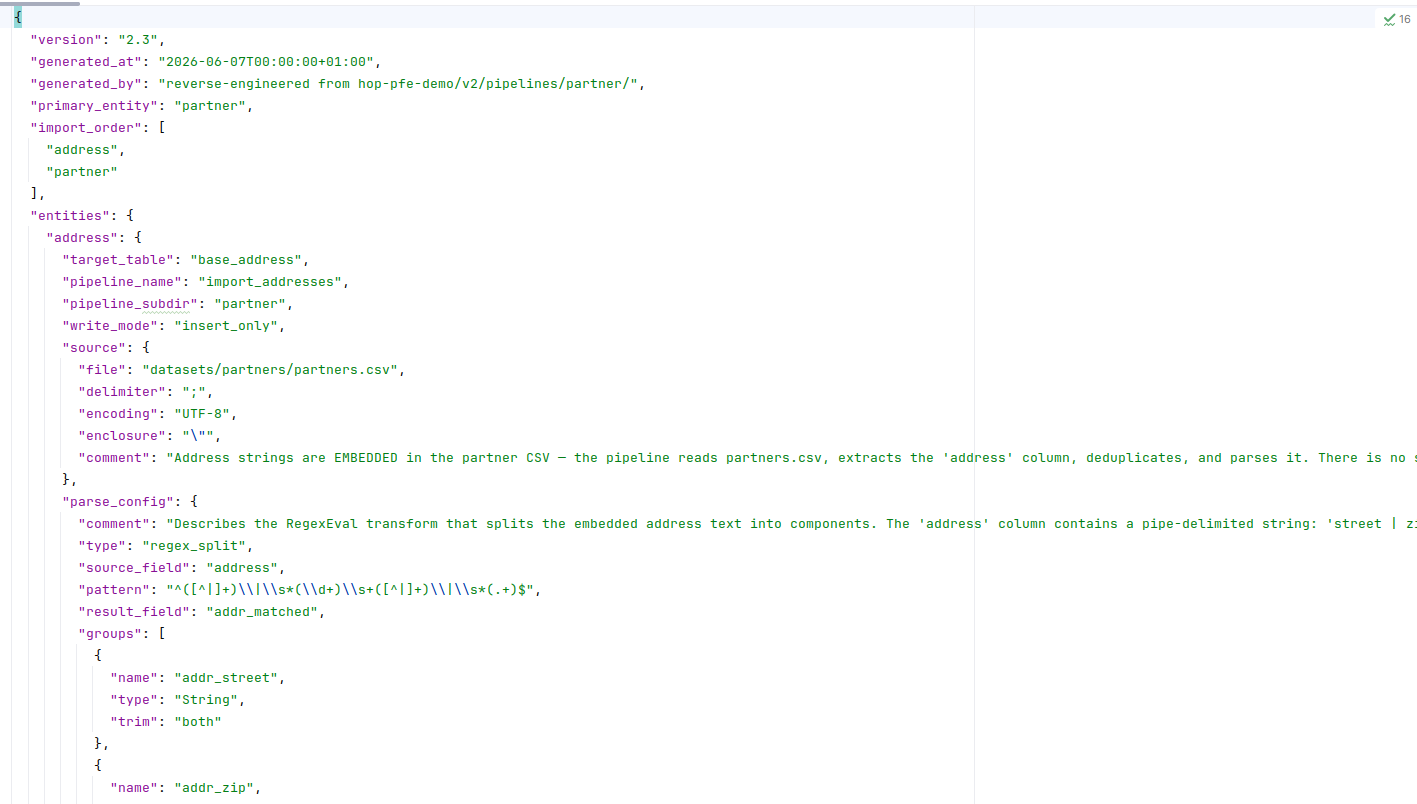
\includegraphics[width=0.8\textwidth]{extrait-manifest.png}
    \caption{Extrait d'un manifeste JSON — section FK resolutions}
    \label{fig:extrait-manifest}
\end{figure}

\subsubsection{Skill generate-pipeline}

Ce skill (1891 lignes + 3 fichiers de référence) transforme un manifeste JSON en fichiers XML Apache Hop. Il opère en cinq étapes~:

\begin{enumerate}
    \item \textbf{Step 0 — Chemins~:} demande à l'utilisateur le chemin du manifeste et le répertoire de sortie pour les fichiers générés.
    \item \textbf{Step 1 — Lecture du manifeste~:} extrait \texttt{import\_order}, les sections entité (table cible, colonnes, FK, champs calculés), ainsi que les \texttt{junction\_pipelines} et \texttt{post\_pipelines}.
    \item \textbf{Step 2 — Lecture des références~:} lit les pipelines de référence existants pour reproduire la structure XML exacte. Trois fichiers de référence fournissent les blocs XML pour chaque type de transform, les conventions critiques (ex~: \texttt{Constant} met la valeur dans \texttt{<nullif>}, pas \texttt{<value>}), et l'architecture standard des chaînes de transforms.
    \item \textbf{Step 3 — Génération~:} pour chaque entité dans \texttt{import\_order}, génère un \texttt{.hpl} en appliquant le pattern approprié~:
    \begin{itemize}
        \item \textbf{Upsert}~: CSV → Select Values → Filter → FK Lookups → Self-lookup → Filter is new → INSERT/UPDATE ;
        \item \textbf{Insert-only}~: CSV → Filter → FK Lookups → Idempotency check → INSERT ;
        \item \textbf{Junction}~: CSV → Lookup side A → Lookup side B → Idempotency check → INSERT jonction ;
        \item \textbf{Post-SQL}~: RowGenerator → ExecSQL (requête SQL directe).
    \end{itemize}
    \item \textbf{Step 5 — Vérification~:} confirme que chaque fichier est du XML valide et rapporte le nombre de fichiers générés.
\end{enumerate}

\begin{figure}[H]
    \centering
    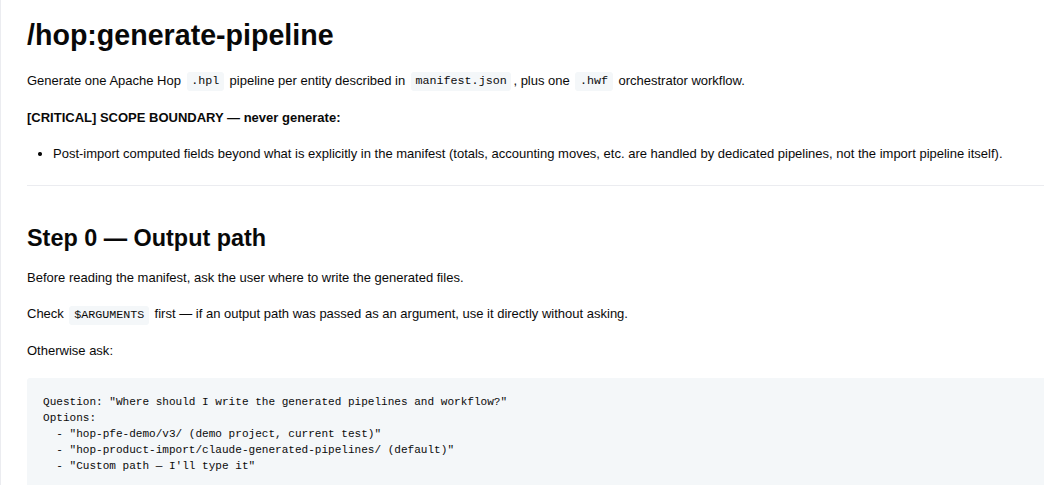
\includegraphics[width=0.7\textwidth]{generate-pipelines-skill.png}
    \caption{Extrait du skill generate-pipeline}
    \label{fig:skill-generate}
\end{figure}

\subsubsection{Skill generate-workflow}

Ce skill (289 lignes + 1 fichier de référence) produit le workflow orchestrateur (\texttt{.hwf}) à partir du manifeste. Il enchaîne les actions dans cet ordre~:

\begin{enumerate}
    \item \textbf{Preflight checks~:} vérification de l'existence du fichier CSV source et test de la connexion BD. En cas d'échec → Abort.
    \item \textbf{Pré-pipelines~:} exécute les pipelines de création de références manquantes (ex~: \texttt{create\_missing\_units}) identifiés par les FK avec \texttt{fk\_source: "embedded"}.
    \item \textbf{Import order~:} exécute séquentiellement chaque pipeline d'entité dans l'ordre topologique. Échec → Abort.
    \item \textbf{Post-pipelines~:} exécute les pipelines de calcul (totaux, taxes, champs dérivés).
    \item \textbf{Junction pipelines~:} exécute les pipelines de liaison M2M.
    \item \textbf{Success~:} action finale si tout a réussi.
\end{enumerate}

Le skill lit deux workflows de référence (v2) pour reproduire le format XML exact, et génère un fichier \texttt{import\_<primary\_entity>.hwf}.

\begin{figure}[H]
    \centering
    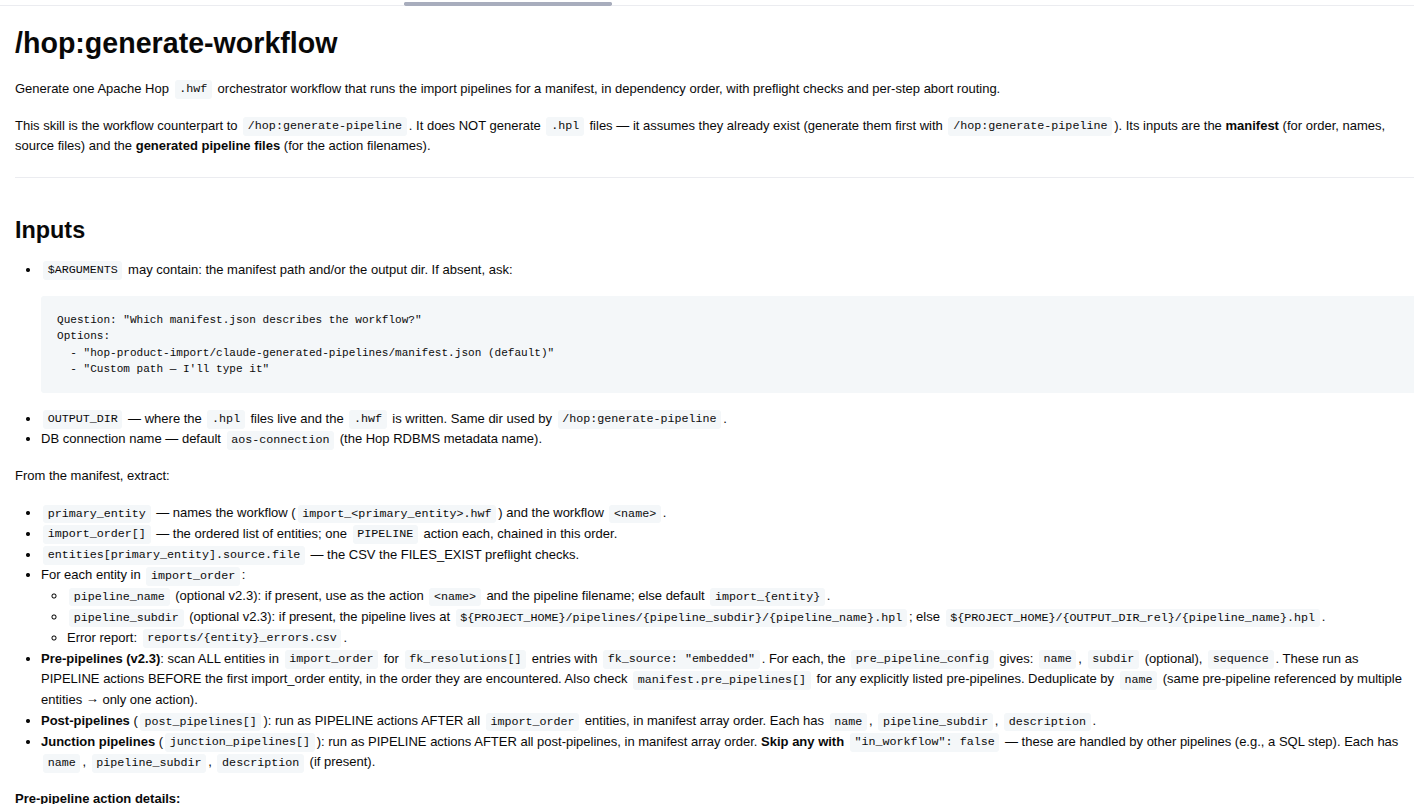
\includegraphics[width=0.7\textwidth]{generate-workflow-skill.png}
    \caption{Extrait du skill generate-workflow}
    \label{fig:skill-workflow}
\end{figure}

\subsubsection{Méthode d'amélioration itérative — Perfect Output}

Après la rédaction initiale des skills, une phase d'amélioration itérative a été appliquée pour augmenter leur fiabilité. La méthode consiste à~:

\begin{enumerate}
    \item \textbf{Créer un dataset de test}~: un jeu de données CSV couvrant les cas de figure à vérifier.
    \item \textbf{Créer manuellement les pipelines et le manifeste de référence}~: ce sont les résultats attendus pour ce dataset.
    \item \textbf{Exécuter le skill}~: lancer l'agent sur le dataset et comparer sa sortie avec la référence.
    \item \textbf{Identifier les écarts}~: chaque différence entre la sortie de l'agent et la référence constitue un défaut du skill.
    \item \textbf{Corriger le skill}~: ajouter les règles, conventions ou exemples manquants dans le prompt ou les fichiers de référence.
    \item \textbf{Itérer}~: relancer jusqu'à convergence (sortie = référence).
\end{enumerate}

Cette boucle a permis de découvrir et documenter de nombreuses conventions non évidentes du XML Apache Hop. À chaque itération, les corrections apportées au skill sont vérifiées manuellement pour s'assurer qu'elles restent généralisables et ne sur-optimisent pas pour un cas particulier (overfitting).

\begin{figure}[H]
    \centering
    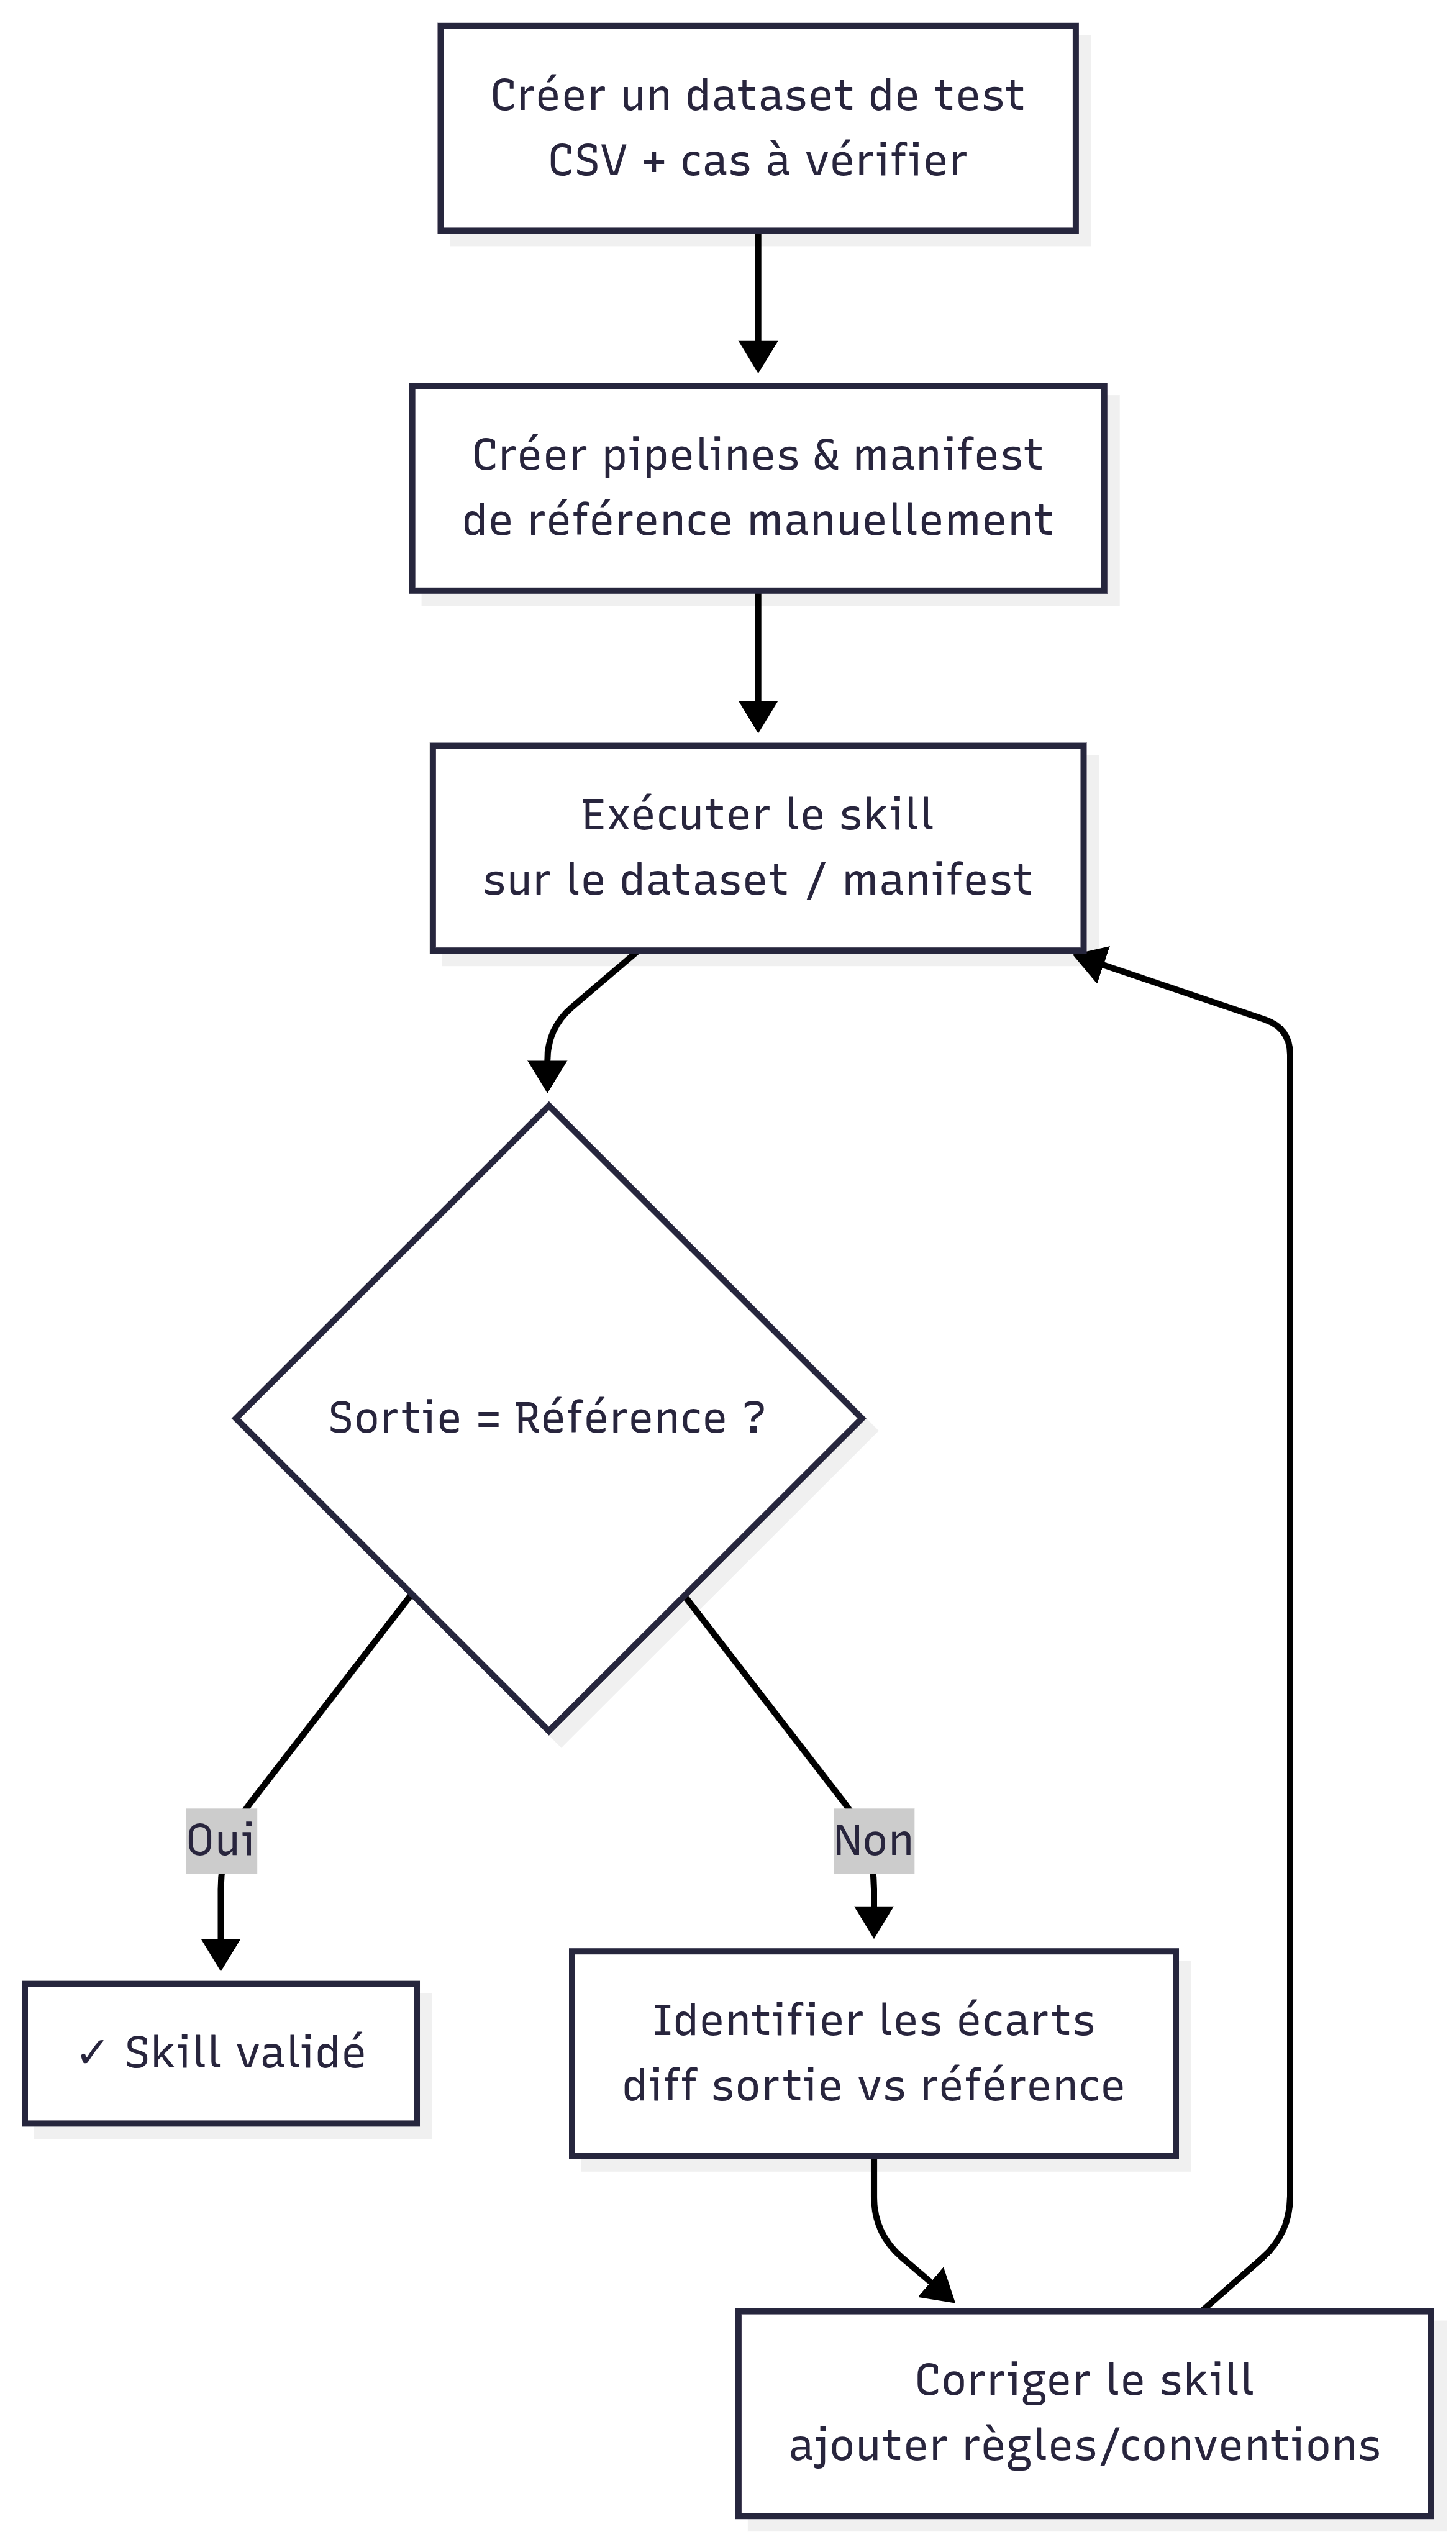
\includegraphics[width=0.7\textwidth]{perfect-output-loop.png}
    \caption{Boucle d'amélioration itérative des skills (Perfect Output)}
    \label{fig:perfect-output}
\end{figure}

%% ──────────────────────────────────────────────────────────────
\subsection{Application Axelor Mapper}

L'application Axelor Mapper est l'interface web qui encapsule l'ensemble du processus d'import. Elle se compose d'un backend FastAPI (Python) et d'un frontend React avec un terminal embarqué (xterm.js).

\subsubsection{Page d'accueil — Sélection de l'entité}

L'utilisateur choisit l'entité cible (produit, partenaire, commande, facture) et saisit les credentials de la base de données PostgreSQL.

\begin{figure}[H]
    \centering
    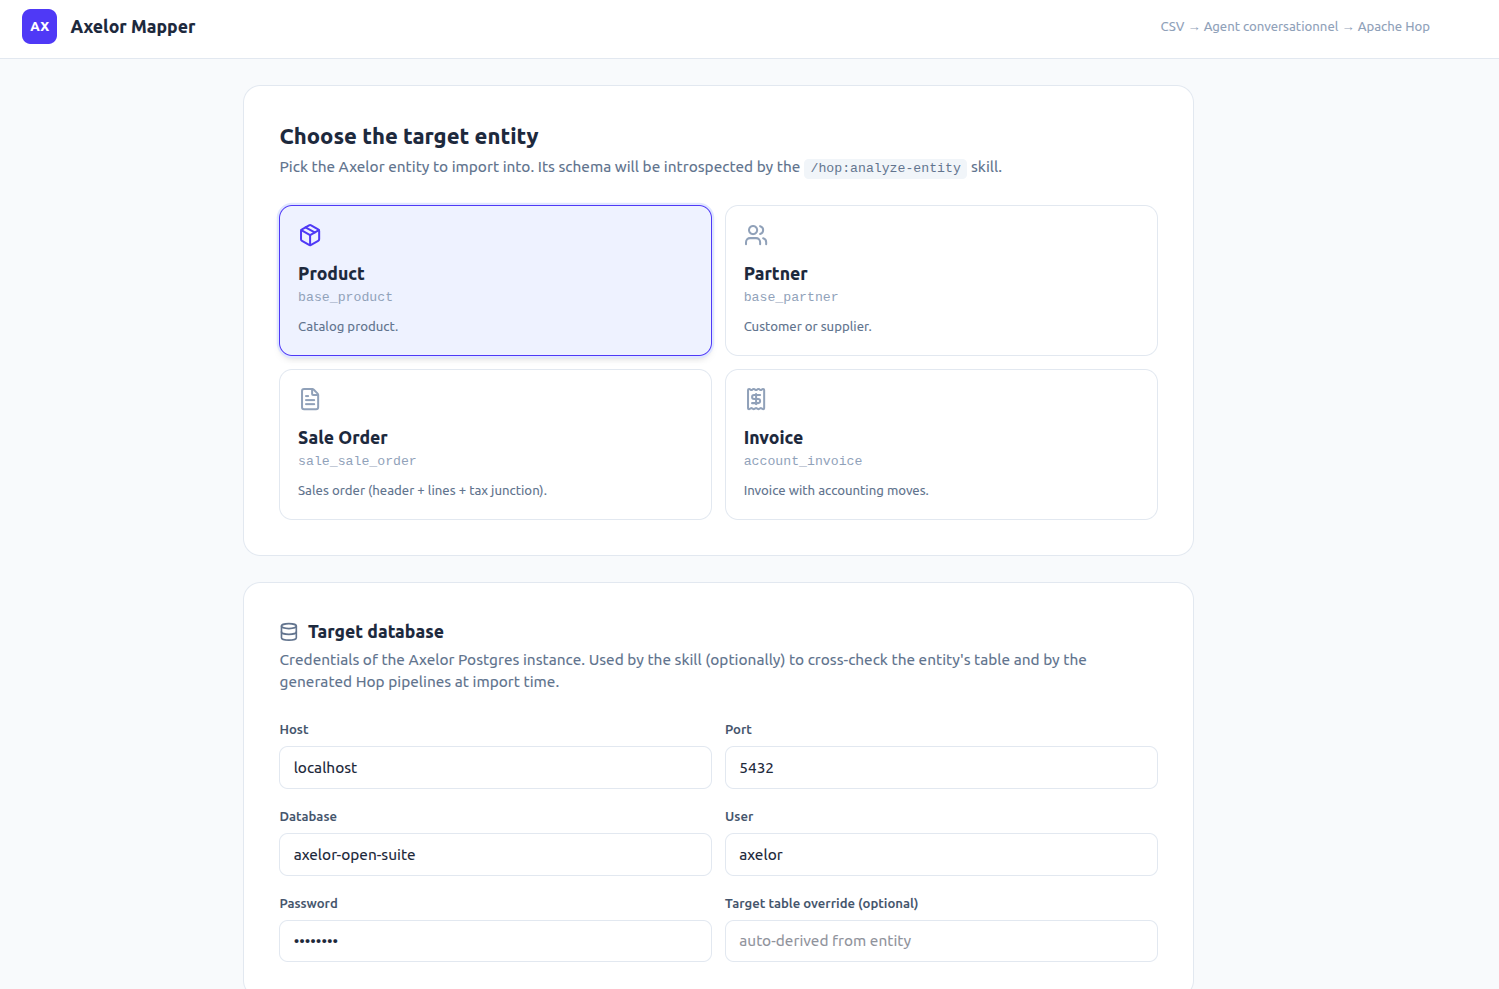
\includegraphics[width=\textwidth]{axelor-mapper-landing-page.png}
    \caption{Page d'accueil — sélection de l'entité et credentials BD}
    \label{fig:mapper-landing}
\end{figure}

\subsubsection{Session conversationnelle — Terminal Claude}

Une fois la session démarrée, un terminal s'ouvre dans le navigateur. L'agent Claude analyse le CSV, pose des questions sur les FK, et demande à l'utilisateur de déposer les fichiers source.

\begin{figure}[H]
    \centering
    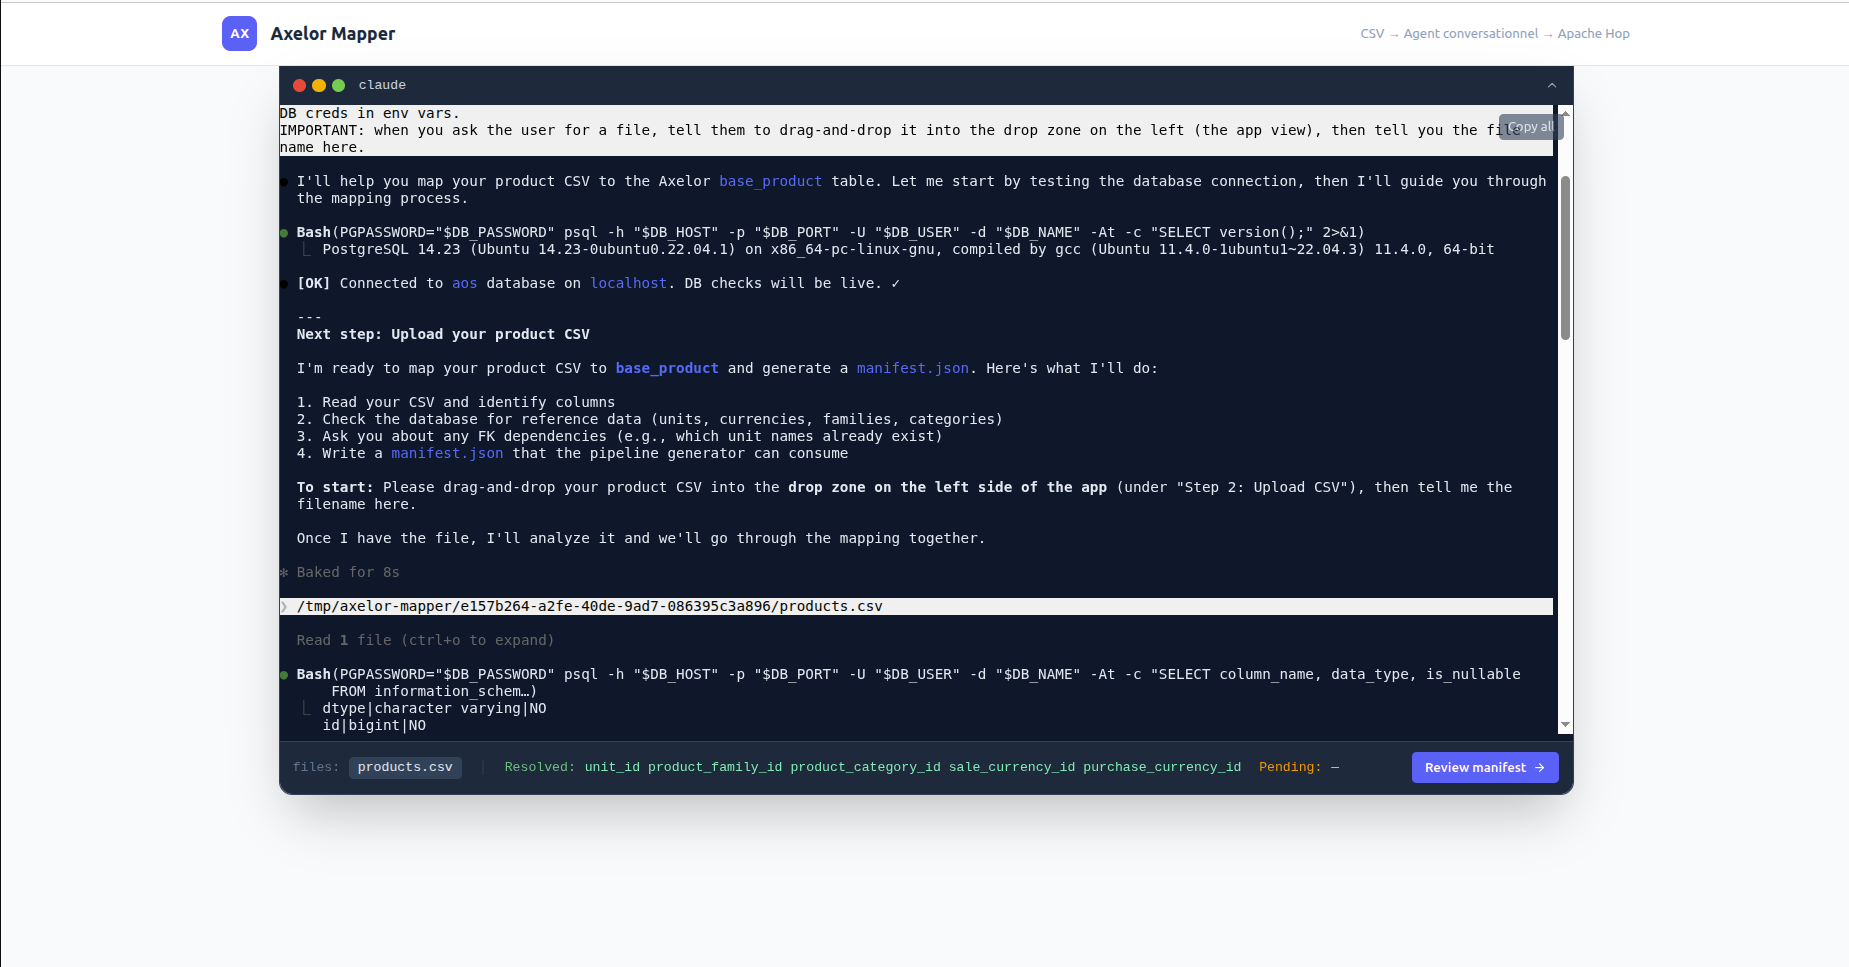
\includegraphics[width=\textwidth]{screenshot-demander-de-drop-le-fichier-source.png}
    \caption{L'agent demande à l'utilisateur de déposer le fichier CSV}
    \label{fig:mapper-drop}
\end{figure}

\begin{figure}[H]
    \centering
    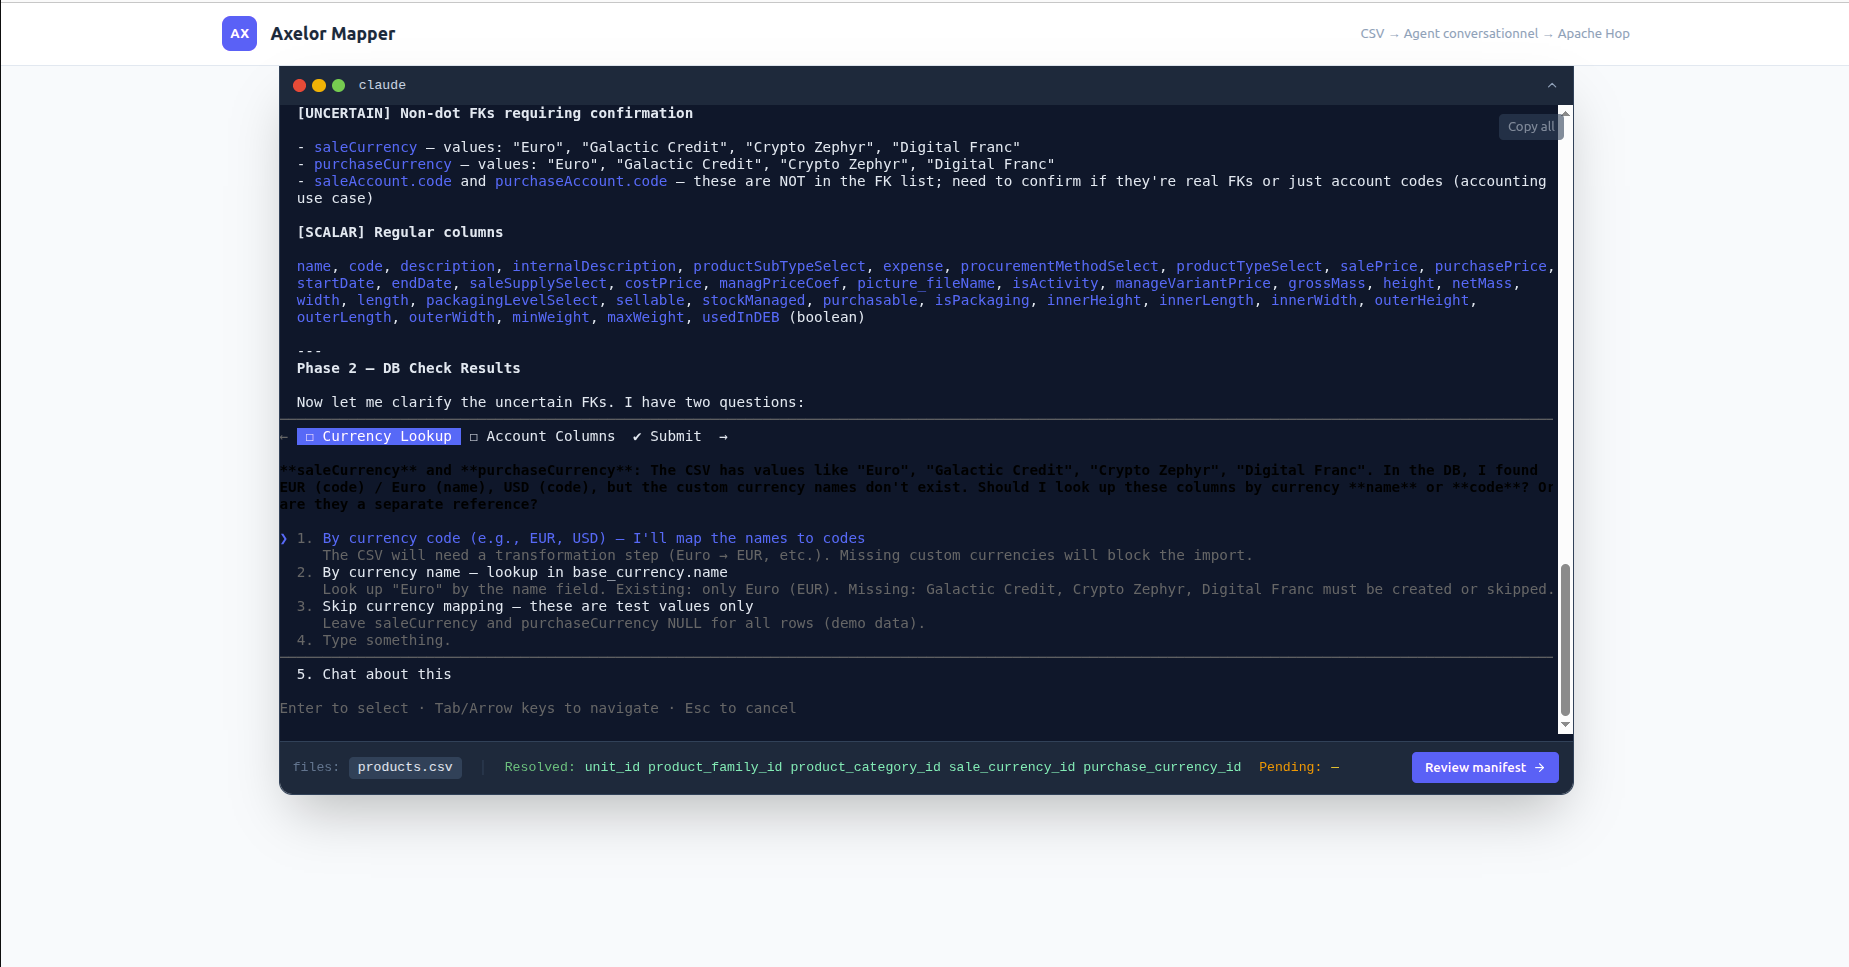
\includegraphics[width=\textwidth]{screenshot-demander-de-confirmation-de-resolution-FK.png}
    \caption{L'agent demande confirmation de la résolution des FK}
    \label{fig:mapper-fk}
\end{figure}

\subsubsection{Génération du manifeste}

L'agent demande le chemin de sortie puis écrit le manifeste JSON.

\begin{figure}[H]
    \centering
    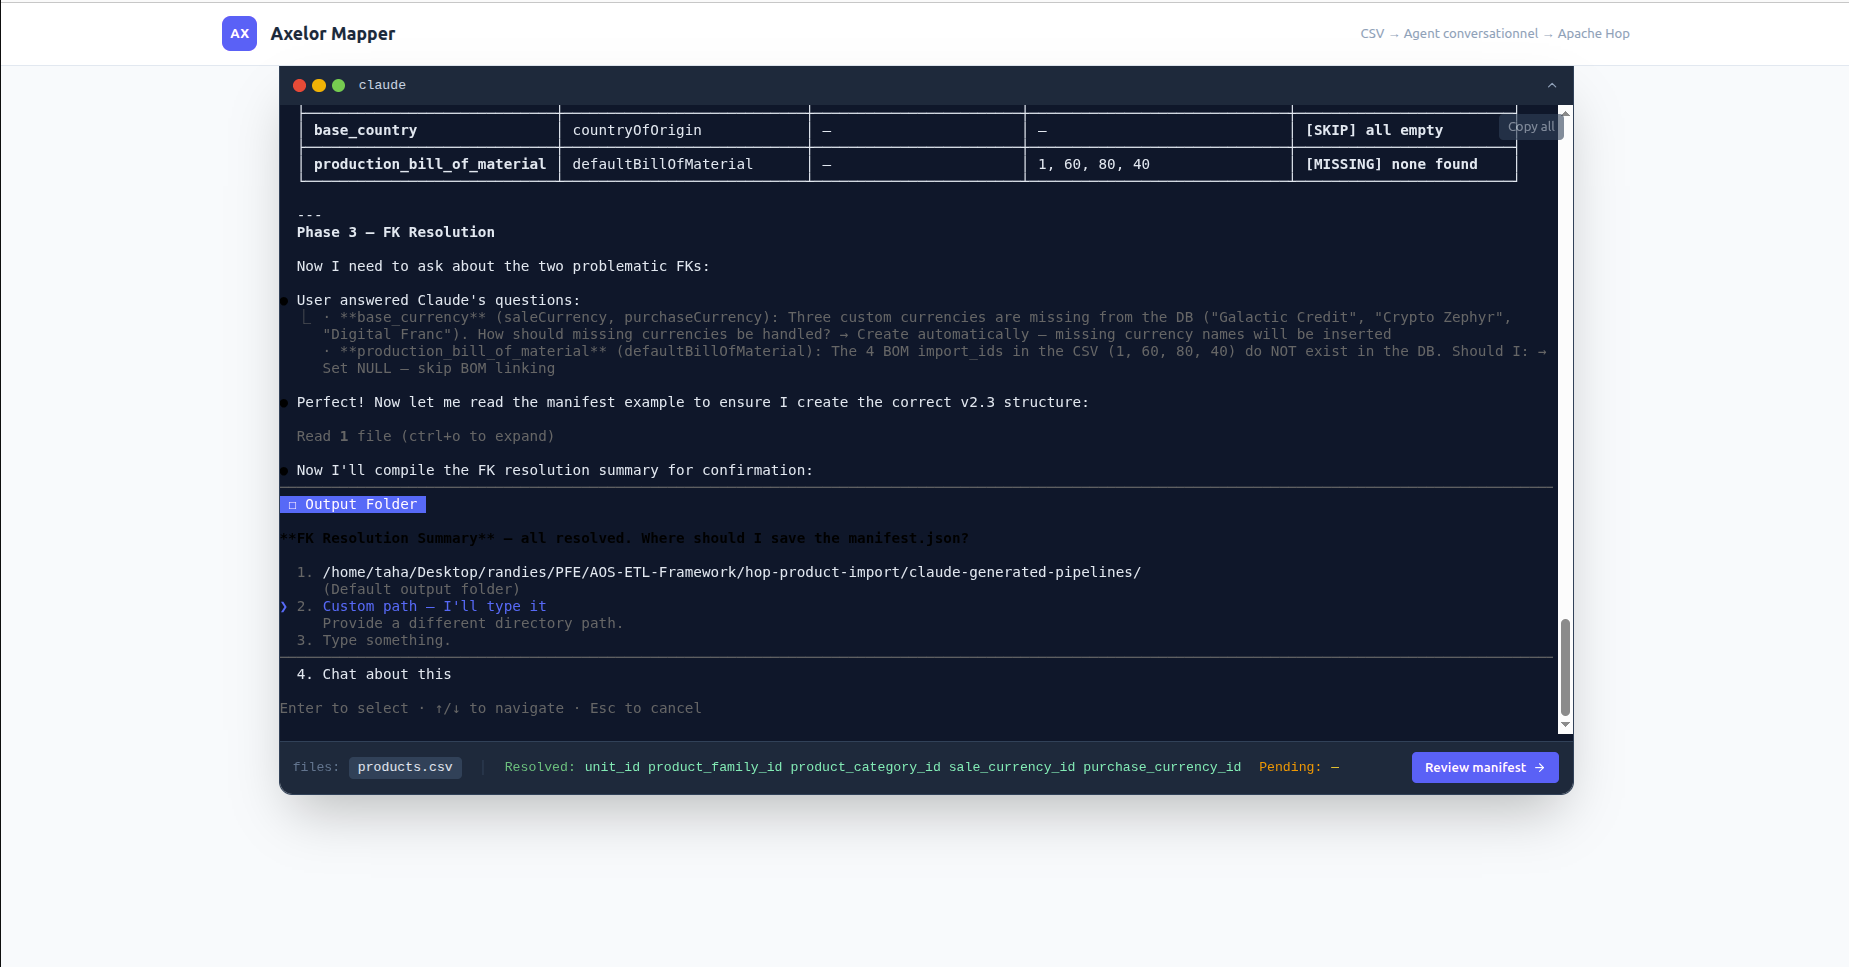
\includegraphics[width=\textwidth]{screenshot-demander-path-creation-manifest.png}
    \caption{L'agent demande où écrire le manifeste}
    \label{fig:mapper-manifest-path}
\end{figure}

\subsubsection{Review du manifeste}

Une fois le manifeste créé, un bouton ``Review Manifest'' apparaît. L'utilisateur peut consulter le mapping proposé avant de passer à la génération.

\begin{figure}[H]
    \centering
    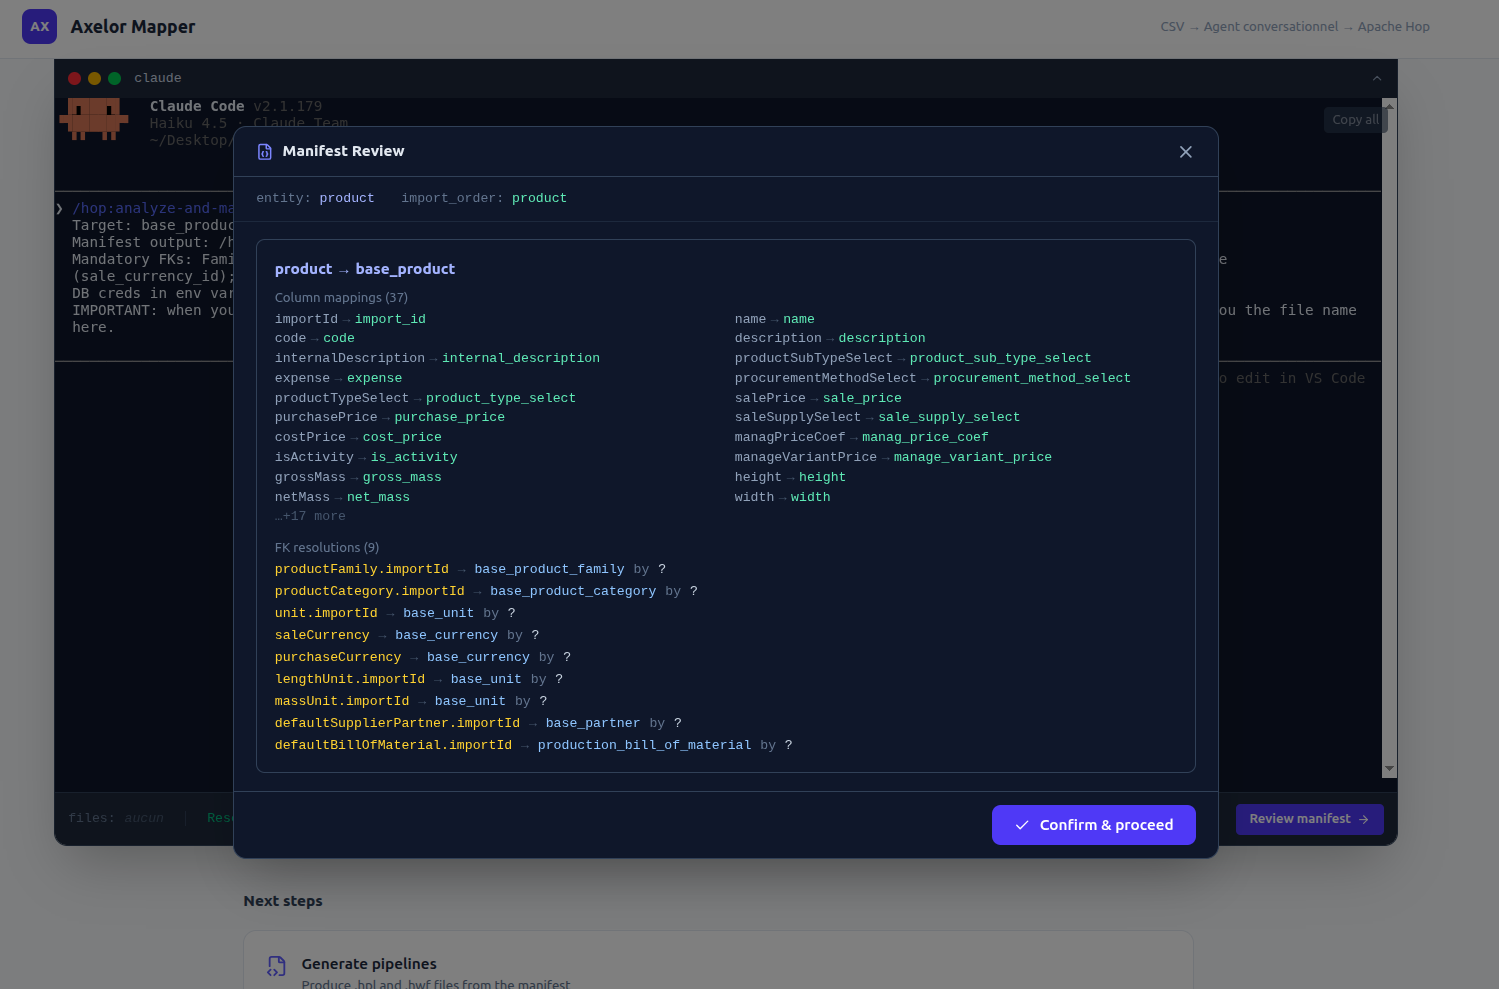
\includegraphics[width=\textwidth]{axelor-mapper-review-manifest.png}
    \caption{Modal de review du manifeste}
    \label{fig:mapper-review}
\end{figure}

\subsubsection{Génération des pipelines}

Après validation du manifeste, l'utilisateur peut lancer la génération des pipelines en spécifiant les chemins (manifeste, données, sortie).

\begin{figure}[H]
    \centering
    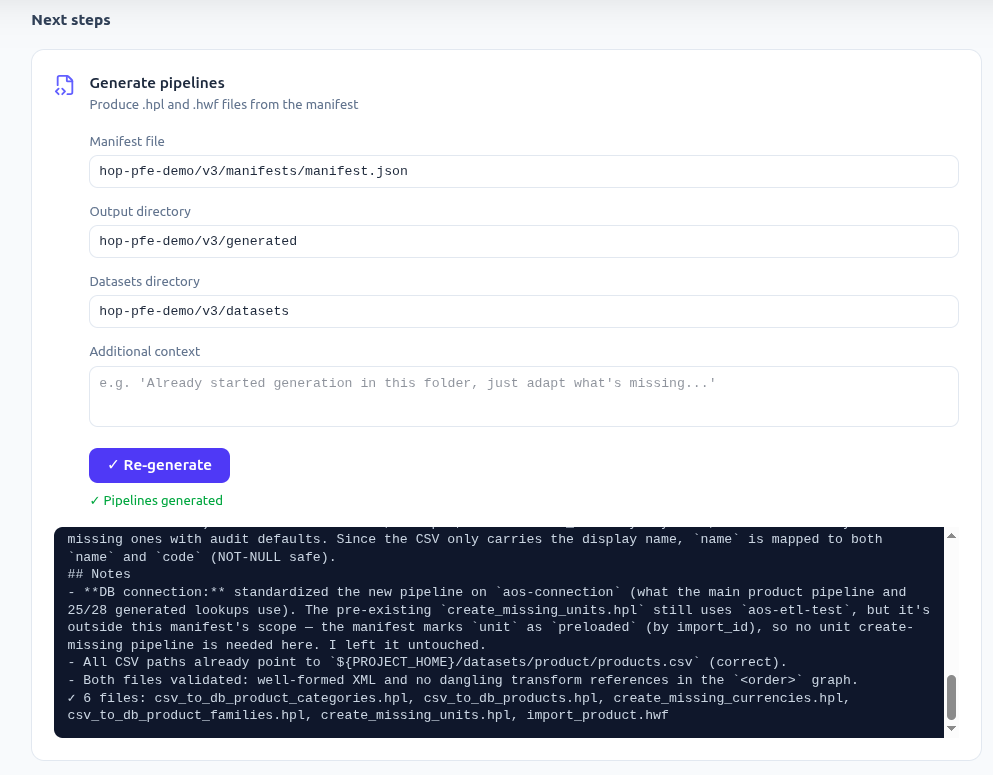
\includegraphics[width=\textwidth]{screenshot-succes-generation-pipelines.png}
    \caption{Génération réussie des pipelines}
    \label{fig:mapper-generate}
\end{figure}

%% ============================================================
\section*{Conclusion}
%% ============================================================

Ce chapitre a présenté l'environnement de développement et l'implémentation des quatre modules d'import (19 pipelines), des 3 skills IA, et de l'application Axelor Mapper. Chaque module suit des patterns adaptés à sa complexité. Le chapitre suivant présente les résultats obtenus et la validation du système.

\chapter{Résultats}
\label{chap:resultats}

Ce chapitre apporte la preuve que la solution fonctionne et répond aux besoins définis. Il présente la stratégie de test, le golden dataset utilisé, les résultats obtenus et le bilan par rapport aux objectifs fixés.

%% ============================================================
\section{Stratégie de test}
%% ============================================================

La validation du framework repose sur un \textbf{golden dataset} — un jeu de données complet et représentatif couvrant l'ensemble des cas de figure rencontrés en production. Ce dataset est conçu pour exercer toutes les fonctionnalités du framework~: résolution de FK par différentes stratégies, gestion des valeurs embarquées, traitement des références manquantes et vérification de l'intégrité référentielle entre entités.

Le critère ultime de conformité est la \textbf{ventilation des factures}~: une facture ne peut être ventilée dans Axelor que si l'ensemble de ses dépendances sont correctement importées (partenaire, adresse, produits, comptes comptables, taxes, conditions de paiement). La ventilation réussie d'une facture prouve donc la cohérence de toute la chaîne d'import.

%% ============================================================
\section{Golden dataset}
%% ============================================================

Le golden dataset est construit pour tester les cas limites suivants~:

\begin{table}[H]
  \centering
  \renewcommand{\arraystretch}{1.4}
  \begin{tabular}{p{4cm} p{9cm}}
    \toprule
    \rowcolor{gray!20}
    \textbf{Caractéristique} & \textbf{Description} \\
    \midrule
    \rowcolor{gray!5}
    Unités embarquées   & Les produits référencent les unités par nom (ex~: ``Jour ouvré'') au lieu d'un import\_id — teste le mode \texttt{fk\_source: embedded} \\
    FK nullables        & Certains produits n'ont pas de BOM (\texttt{defaultBillOfMaterial} = null) — teste la tolérance aux FK optionnelles \\
    \rowcolor{gray!5}
    Adresses embarquées & Les partenaires contiennent l'adresse en texte libre (``70 RUE PASTORELLI | 06000 NICE | FRANCE'') — teste le parsing et la création d'adresses \\
    Taxes embarquées    & Les lignes de commandes et factures référencent les taxes par code — teste la résolution FK multi-niveaux \\
    \rowcolor{gray!5}
    Volume              & 75 produits, 68 partenaires, 1\,000 commandes (3\,987 lignes), 1\,000 factures (3\,974 lignes) avec leurs lignes et jonctions \\
    \bottomrule
  \end{tabular}
  \caption{Caractéristiques du golden dataset}
  \label{tab:golden-dataset}
\end{table}

%% ============================================================
\section{Tests effectués}
%% ============================================================

\subsection{Tests d'import par entité}

\begin{table}[H]
  \centering
  \renewcommand{\arraystretch}{1.4}
  \begin{tabular}{p{4cm} p{2.5cm} p{2.5cm} p{4cm}}
    \toprule
    \rowcolor{gray!20}
    \textbf{Entité} & \textbf{Lignes CSV} & \textbf{Importées} & \textbf{Erreurs} \\
    \midrule
    \rowcolor{gray!5}
    Unités (create\_missing) & 5  & 5  & 0 \\
    Familles produit         & 14 & 14 & 0 \\
    \rowcolor{gray!5}
    Catégories produit       & 18 & 18 & 0 \\
    Produits                 & 75 & 72 & 3 \\
    \rowcolor{gray!5}
    Adresses                 & 68 & 64 & 4 \\
    Partenaires              & 68 & 64 & 4 \\
    \rowcolor{gray!5}
    Commandes de vente       & 1\,000 & 962 & 38 \\
    Lignes de commande       & 3\,987 & 3\,987 & 0 \\
    \rowcolor{gray!5}
    Factures                 & 1\,000 & 950 & 50 \\
    Lignes de facture        & 3\,974 & 3\,974 & 0 \\
    \bottomrule
  \end{tabular}
  \caption{Résultats d'import par entité}
  \label{tab:resultats-import}
\end{table}

Les erreurs rencontrées correspondent à des cas volontairement introduits dans le dataset pour valider le comportement du framework face aux données incorrectes~:
\begin{itemize}
    \item \textbf{Produits (3 erreurs)~:} lignes dont le champ \texttt{name} était vide — rejetées car champ obligatoire ;
    \item \textbf{Partenaires et adresses (4 erreurs)~:} partenaires dont le partenaire parent (\texttt{parentPartner}) ne pouvait pas être résolu — la ligne partenaire et l'adresse associée sont rejetées ensemble ;
    \item \textbf{Commandes de vente (38 erreurs)~:} commandes rejetées en raison d'une référence manquante non résolvable ;
    \item \textbf{Factures (50 erreurs)~:} factures dont le statut (\texttt{statusSelect}) était absent — champ requis pour la ventilation.
\end{itemize}
Les lignes de détail (lignes de commande et lignes de facture) ne sont pas comptabilisées en erreur~: elles sont simplement non traitées lorsque leur document parent est rejeté.

\subsection{Test de conformité — Ventilation des factures}

Le critère de conformité retenu est la \textbf{ventilation} des factures dans Axelor Open Suite. Une facture ne peut être ventilée que si l'ensemble de ses dépendances sont correctement importées et liées~: partenaire, adresse de facturation, produits, comptes comptables, taxes et conditions de paiement. Le test vérifie également que~:

\begin{itemize}
    \item Les \textbf{mouvements comptables} (\emph{account move}) sont générés à la ventilation ;
    \item Les \textbf{lignes de mouvement} (\emph{move lines}) — débit et crédit — sont créées avec les bons montants et comptes.
\end{itemize}

\textbf{Résultat~:} la ventilation s'est exécutée avec succès. Les mouvements et lignes de mouvement ont été créés correctement, confirmant l'intégrité référentielle de l'ensemble de la chaîne d'import.

\subsection{Test d'idempotence}

Le workflow complet a été exécuté une seconde fois sur le même dataset. Résultat attendu~: aucun doublon créé, les enregistrements existants sont mis à jour uniquement si modifiés.

\textbf{Résultat~:} 0 insertions, 0 mises à jour (données inchangées) — le mécanisme d'upsert via \texttt{import\_id} fonctionne correctement.

%% ============================================================
\section{Analyse des performances}
%% ============================================================

Le golden dataset intègre à la fois les cas limites fonctionnels et un volume suffisant pour évaluer les performances~: \textbf{1\,000 commandes} (3\,987 lignes) et \textbf{1\,000 factures} (3\,974 lignes), référençant exclusivement les \texttt{import\_id} de partenaires, contacts et produits importés au préalable dans la base \texttt{axelor\_etl\_test\_v2}.

\subsection{Protocole de mesure}

Les performances sont mesurées par chronométrage du temps mural (\emph{wall-clock}) de chaque workflow, sur une insertion à froid (plages d'\texttt{import\_id} initialement vides). Le débit est exprimé en lignes traitées par seconde (en-tête + lignes de détail).

\subsection{Résultats du framework}

\begin{table}[H]
  \centering
  \renewcommand{\arraystretch}{1.4}
  \begin{tabular}{p{3.5cm} p{2cm} p{2cm} p{3cm} p{2cm}}
    \toprule
    \rowcolor{gray!20}
    \textbf{Entité} & \textbf{Documents} & \textbf{Lignes} & \textbf{Temps} & \textbf{Débit} \\
    \midrule
    \rowcolor{gray!5}
    Commandes de vente & 1\,000 & 4\,987 & 344~s ($\approx$5\,min\,44) & $\approx$14,5~l/s \\
    Factures           & 1\,000 & 4\,974 & 298~s ($\approx$4\,min\,58) & $\approx$16,7~l/s \\
    \rowcolor{gray!5}
    \textbf{Total}     & \textbf{2\,000} & \textbf{9\,961} & \textbf{642~s ($\approx$10\,min\,42)} & --- \\
    \bottomrule
  \end{tabular}
  \caption{Performances du framework sur le jeu de volume}
  \label{tab:perf-framework}
\end{table}

Aucune ligne n'a été rejetée et toutes les clés étrangères ont été résolues (0 produit, client ou partenaire non résolu). Le débit reste modéré car le framework effectue une résolution de FK ligne par ligne (\emph{Database Lookup}) avant l'écriture~: il ne s'agit pas d'une insertion en masse brute. Ces valeurs correspondent à une mesure préliminaire (un seul run, démarrage à froid incluant l'amorçage de la JVM Hop)~; la version finale retiendra la médiane sur cinq exécutions.

\subsection{Comparaison avec l'import natif d'Axelor}

Le mécanisme natif d'Axelor (binding XML \texttt{<csv-inputs>} traité par \texttt{CSVImporter}) fait transiter chaque enregistrement par la couche applicative~: requête de recherche pour l'upsert, requête par clé étrangère, puis persistance Hibernate complète (verrou optimiste, champs d'audit, écouteurs métier). Cette logique par enregistrement est plus coûteuse que l'écriture en \emph{staging} du framework. Les deux approches ont été mesurées sur le même jeu de données~; les résultats sont présentés dans le tableau ci-dessous.

\begin{table}[H]
  \centering
  \renewcommand{\arraystretch}{1.4}
  \begin{tabular}{p{4cm} p{4cm} p{4cm}}
    \toprule
    \rowcolor{gray!20}
    \textbf{Entité} & \textbf{Framework (mesuré)} & \textbf{Natif (mesuré)} \\
    \midrule
    \rowcolor{gray!5}
    Commandes & 344~s & $\approx$11 à 29~min \\
    Factures  & 298~s & $\approx$10 à 25~min \\
    \rowcolor{gray!5}
    \textbf{Total} & \textbf{$\approx$10,7~min} & \textbf{$\approx$20 à 55~min} \\
    \bottomrule
  \end{tabular}
  \caption{Comparaison framework vs import natif Axelor (mesures sur le même jeu de données)}
  \label{tab:perf-comparaison}
\end{table}


%% ============================================================
\section{Valeur ajoutée du projet}
%% ============================================================

\begin{itemize}
    \item \textbf{Réutilisabilité} : les règles d'import sont déclaratives (mapping, transformations, résolution FK) et réutilisables d'un client à l'autre, là où l'approche historique reposait sur des scripts Java jetables.
    \item \textbf{Autonomie vis-à-vis de l'application} : l'écriture directe en base, avec respect de l'intégrité référentielle et des champs d'audit, libère l'import de la disponibilité d'une instance Axelor et de sa couche ORM.
    \item \textbf{Gestion native des formats} : les formats français (date \texttt{jj/mm/aaaa}, décimale à virgule, espaces de milliers) sont traités de façon déclarative, sans écriture d'adaptateurs Java comme l'exige l'import natif.
    \item \textbf{Performance} : sur le jeu de volume, le framework charge 2\,000 documents et près de 10\,000 lignes en environ 10~minutes, avec une marge d'optimisation (lookups, taille des lots) encore disponible.
    \item \textbf{Accélération du cycle de configuration} : couplé aux skills IA et à l'application Mapper, le temps de mise en place d'un nouvel import est fortement réduit.
\end{itemize}

%% ============================================================
\section{Bilan des réalisations}
%% ============================================================

\begin{table}[H]
  \centering
  \renewcommand{\arraystretch}{1.4}
  \begin{tabular}{p{7cm} p{2.5cm} p{4cm}}
    \toprule
    \rowcolor{gray!20}
    \textbf{Objectif} & \textbf{Statut} & \textbf{Commentaire} \\
    \midrule
    \rowcolor{gray!5}
    Standardiser l'import via pipelines ETL  & Couvert     & 19 pipelines couvrant 4 domaines \\
    Valider sur 4 entités représentatives    & Couvert     & Golden dataset importé et ventilé \\
    \rowcolor{gray!5}
    Automatiser via agents IA                & Couvert     & Skill analyze-and-map fonctionnel \\
    Générer les pipelines par IA             & Partiel     & Cas simples fonctionnels, cas complexes nécessitent du tuning \\
    \rowcolor{gray!5}
    Application Mapper                       & Couvert     & Interface complète (terminal + next steps) \\
    Idempotence des imports                  & Couvert     & Testé et validé \\
    \rowcolor{gray!5}
    Performance (volumétrie)                 & Couvert     & Benchmark sur 2\,000 documents ($\approx$10\,min) \\
    \bottomrule
  \end{tabular}
  \caption{Bilan par rapport aux objectifs}
  \label{tab:bilan}
\end{table}

%% ============================================================
\section*{Conclusion}
%% ============================================================

Les tests sur le golden dataset ont démontré que le framework AOS-ETL répond aux objectifs fixés. L'import complet des 4 domaines d'entités avec ventilation réussie des factures valide l'intégrité de la chaîne. Le mécanisme d'upsert garantit l'idempotence. La génération de pipelines par IA, bien que fonctionnelle pour les cas standards, reste un axe d'amélioration pour les entités complexes.

\chapter*{Conclusion Générale et Perspectives}
\addcontentsline{toc}{chapter}{Conclusion Générale et Perspectives}
\markboth{Conclusion Générale et Perspectives}{Conclusion Générale et Perspectives}

\vspace{0.5cm}

Ce projet de fin d'études a porté sur la conception et la réalisation d'un framework ETL à gateways de décision pour l'import ERP, développé au sein de la société Axelor. Face à la prolifération de scripts Java non réutilisables imposant un effort de développement conséquent à chaque nouveau projet client, l'objectif était de proposer une solution standardisée, déclarative et assistée par intelligence artificielle, permettant à tout consultant fonctionnel d'importer des données dans Axelor Open Suite sans compétences en développement Java.

% ─────────────────────────────────────────────────────────────
\section*{Rappel de la problématique et des objectifs}
% ─────────────────────────────────────────────────────────────

La problématique initiale portait sur l'absence de standardisation des migrations de données au sein des projets Axelor : chaque client nécessitait un ensemble de scripts Java développés sur mesure, non réutilisables d'un projet à l'autre, inaccessibles aux consultants fonctionnels et impossibles à maintenir sans compétences en développement Java. L'analyse de trois projets réels — \textit{bolt-app} (23~scripts), \textit{neodyme} (20~scripts) et \textit{xelians} (3~configurations XML) — a mis en évidence le coût humain de cette situation et l'urgence d'une capitalisation transversale.
L'objectif du projet était de concevoir un framework ETL basé sur Apache Hop, couvrant les quatre domaines fonctionnels essentiels d'Axelor Open Suite — Base, CRM, Ventes et Achats —, de l'enrichir par trois \textit{skills} d'intelligence artificielle pour assister la configuration des pipelines, et de le rendre accessible à travers une application web de mapping, l'\textit{Axelor Mapper}.

% ─────────────────────────────────────────────────────────────
\section*{Bilan des réalisations}
% ─────────────────────────────────────────────────────────────

Les objectifs fixés en début de projet ont été atteints. La solution livrée apporte :

\begin{itemize}
  \item \textbf{un framework ETL réutilisable et paramétrable}, couvrant l'import de quatre entités Axelor — Produit, Partenaire, Commande de vente et Facture — à travers des pipelines Apache Hop standardisés et modulaires, organisés selon une architecture en deux étapes (consolidation puis injection) garantissant la cohérence transactionnelle ;
  \item \textbf{un assistant IA de configuration}, composé de trois \textit{skills} Claude — \texttt{analyze-and-map-entity}, \texttt{generate-pipeline} et \texttt{generate-workflow} — qui automatisent l'analyse du fichier source, la résolution interactive des clés étrangères et la génération des fichiers \texttt{.hpl}/\texttt{.hwf} ;
  \item \textbf{un contrat d'interface déclaratif}, le manifeste JSON, servant d'artefact intermédiaire entre l'analyse conversationnelle et la génération des pipelines, versionnable sous Git et régénérable à la demande sans ré-analyse ;
  \item \textbf{une application web accessible}, l'\textit{Axelor Mapper}, offrant au consultant une interface graphique pour sélectionner l'entité cible, déposer le fichier source et piloter la session conversationnelle Claude via un terminal PTY intégré ;
  \item \textbf{une validation complète sur jeu de données \textit{golden}}, confirmant la conformité des imports, l'idempotence des pipelines et des performances nettement supérieures à l'import natif Axelor sur les volumes testés.
\end{itemize}

La validation conduite sur un jeu de données réaliste — 75~produits, 68~partenaires, 1000~commandes de vente et 1000~factures avec ventilation comptable — ainsi que les mesures de performance recueillies, ont confirmé la fiabilité de la solution et sa conformité à l'ensemble des besoins fonctionnels et non fonctionnels exprimés.

% ─────────────────────────────────────────────────────────────
\section*{Apports du stage}
% ─────────────────────────────────────────────────────────────

Ce stage a constitué une expérience particulièrement enrichissante, tant sur le plan technique que professionnel.
Il a permis de :

\begin{itemize}
  \item maîtriser l'architecture et les conventions d'Apache Hop dans un contexte d'intégration ERP réel, en appréhendant les subtilités des \textit{transforms}, des workflows et des contraintes de contournement de l'ORM Axelor ;
  \item acquérir une expertise concrète en \textit{prompt engineering} appliqué à la génération de code technique structuré, notamment la conception de \textit{skills} conversationnels capables de produire du XML Hop valide à partir d'une description déclarative ;
  \item développer des compétences en développement \textit{full-stack} : conception d'une API FastAPI, d'une interface React avec terminal intégré xterm.js, et orchestration d'une session Claude via PTY WebSocket ;
  \item renforcer la capacité à analyser un besoin métier complexe — ici la migration de données ERP avec gestion des clés étrangères, des contraintes d'intégrité référentielle et des séquences PostgreSQL — et à le traduire en une solution technique structurée, testée et documentée ;
  \item s'intégrer au sein d'une équipe de consultants Axelor et adopter les pratiques professionnelles de gestion de projet incrémental, de versionnement et de livraison itérative.
\end{itemize}

Cette immersion au c\oe{}ur d'un projet à forte valeur métier a consolidé une vision d'ensemble de l'ingénierie des données et de l'intégration de systèmes d'information, et constitue un tremplin précieux vers une carrière dans la mise en \oe{}uvre de solutions ERP et d'architectures ETL.

% ─────────────────────────────────────────────────────────────
\section*{Perspectives d'évolution}
% ─────────────────────────────────────────────────────────────

La solution réalisée constitue un socle robuste sur lequel plusieurs évolutions à forte valeur ajoutée sont d'ores et déjà envisagées.

L'axe d'évolution prioritaire est l'extension du framework à de nouveaux domaines fonctionnels d'Axelor Open Suite, notamment les \textbf{ordres de fabrication} (\textit{Manufacturing Order}) et les \textbf{mouvements de stock} (\textit{Stock Move}). Ces entités présentent des contraintes de cohérence plus exigeantes — liens avec les nomenclatures, les emplacements et les lots de traçabilité — et constitueront un véritable test de la généricité de l'architecture de \textit{gateway pipeline}.

Un second axe majeur concerne l'\textbf{élargissement des sources de données} supportées. La version actuelle traite exclusivement des fichiers CSV ; or, les projets d'intégration Axelor mobilisent des sources bien plus variées : fichiers Excel, bases de données relationnelles externes (PostgreSQL, MySQL), bases documentaires (MongoDB) ou encore exports XML issus d'autres ERP. Étendre le framework à ces formats permettrait de couvrir l'essentiel des contextes clients sans modifier les pipelines d'import aval.

Ces deux axes s'accompagnent d'un troisième, étroitement lié : l'intégration d'un \textbf{rapport de qualité de données} avant import. Ce mécanisme permettrait de détecter et de qualifier les anomalies de chaque ligne source — champs requis manquants, clés étrangères inexistantes, formats non conformes — avant toute écriture en base de données, réduisant significativement les itérations de correction et offrant au consultant une visibilité complète sur l'état de ses données avant toute mise en production.

D'autres pistes complètent cette vision : l'amélioration des \textit{skills} IA par capitalisation sur l'historique des mappings réussis pour proposer des configurations de plus en plus pertinentes, la \textbf{publication en open source} du framework afin de favoriser les contributions de la communauté Axelor, et la \textbf{généralisation au-delà d'Axelor} par abstraction de la couche de mapping pour supporter d'autres ERP open source tels qu'Odoo ou ERPNext.

\vspace{0.5cm}

En définitive, ce projet a permis de livrer un framework ETL pleinement opérationnel, aligné sur les besoins réels des projets d'intégration Axelor, tout en traçant une trajectoire d'évolution ambitieuse vers un outillage intelligent et communautaire de migration de données ERP.


% ── Bibliographie ───────────────────────────────────────────
\printbibliography[heading=bibintoc, title={R\'ef\'erences}, nottype=misc]
\printbibliography[heading=bibintoc, title={Webographie}, type=misc]

\end{document}
